\documentclass{report}
\usepackage[utf8]{inputenc}
% Images setup
\usepackage{graphicx}
\graphicspath{ {imagenes/} }
% Page layout setup
\usepackage[a4paper,width=150mm,top=25mm,bottom=25mm]{geometry}
% Headers and footers setup
\usepackage{fancyhdr}
\pagestyle{fancy}
% Document language setup
\usepackage[spanish]{babel}
% Bibliography
\usepackage[backend=biber, style=alphabetic, citestyle=alphabetic]{biblatex}
\usepackage{csquotes}
\addbibresource{references.bib}
% Pretty hyperlinks
\usepackage[hidelinks]{hyperref}
% Allows to cross reference other chapters
\usepackage{nameref}
% Allows to use multipage tables
\usepackage{longtable, tabu}
\usepackage{array}
%Allows horitontal pages
\usepackage{pdflscape}
% Numerate subsections and include in the content table
\setcounter{secnumdepth}{4}
\setcounter{tocdepth}{3}
% Makes images appear in the section they belong to
\usepackage[section]{placeins}
% Block comments
\usepackage{comment}
% Paragraph spacing
\usepackage{parskip}
\setlength{\parindent}{1.5em}
\setlength{\parskip}{1em}
% Adjust image position
\usepackage{subcaption}


\begin{document}
\begin{titlepage}
\begin{center}

% Upper part of the page. The '~' is needed because \\
% only works if a paragraph has started.


~\\[2cm]
\textsc{\textbf{\LARGE Universidad de Oviedo}}\\[.5cm]

\begin{figure}
\centering
\begin{minipage}{.5\textwidth}
  \centering
  
\includegraphics[width=.4\linewidth]{logos/eii}
\end{minipage}%
\begin{minipage}{.5\textwidth}
  \centering
  
\includegraphics[width=.4\linewidth]{logos/uniovi}
\end{minipage}
\end{figure}

~\\[1cm]

\textsc{\Large Escuela de Ingeniería Informática}\\[1cm]

\textsc{\textbf{\Large Trabajo Fin de Grado}}\\[1.5cm]

% Title
~\\[1cm]
{ \huge \bfseries Backend de un portal de datos e información sobre la Tierra \\[0.4cm] }
~\\[6cm]

% Author and supervisor
\begin{minipage}{0.4\textwidth}
	\begin{flushleft} \large
		\emph{Autor:}\\
		Cristian Álvarez Belaustegui
	\end{flushleft}
\end{minipage}
\begin{minipage}{0.4\textwidth}
	\begin{flushright} \large
		\emph{Director:} \\
		Jose Emilio Labra Gayo
	\end{flushright}
\end{minipage}

\vfill

\end{center}
\end{titlepage}

\newpage
\thispagestyle{plain}
\mbox{}

\chapter*{Agradecimientos}
\label{agradecimientos}
A mis padres, quienes siempre me han demostrado el valor del trabajo, la dedicación
y las cosas bien hechas.  A mi hermana, porque su esfuerzo sirvió en gran parte 
como inspiración en los momentos de flaqueza.  A mi novia, quien me apoyó en todo
momento y sin la cual nada sería lo mismo.  A mi director y a todos los miembros de WESO, 
por crear un ambiente de trabajo en el que hasta los momentos más duros merecieron
la pena.

\newpage
\thispagestyle{plain}
\mbox{}

\chapter*{Resumen}
\label{resumen}
asf

\newpage
\thispagestyle{plain}
\mbox{}

\tableofcontents
\addcontentsline{toc}{chapter}{Agradecimientos}
\addcontentsline{toc}{chapter}{Resumen}

\listoffigures

\listoftables

\chapter{Introducción}
\label{chapter01}
\section{Justificación del Proyecto}
El presente proyecto tiene como objetivo la construcción de un backend para un portal de datos sobre la tierra.  Éste proyecto forma parte a su vez del proyecto \textit{Rebuilding IFAD's LandPortal RFQ/2013/016/SC} desarrollado por el grupo de investigación Web Semantics Oviedo\footnote{WESO - http://www.weso.es/} y la empresa {SB Consulting\footnote{SBC4D - http://www.sbc4d.com/} y que cuenta como cliente con el Fondo Internacional para el Desarrollo Agrícola\footnote{IFAD - http://www.ifad.org/}, perteneciente a la Organización de las Naciones Unidas\footnote{ONU - http://www.un.org/es/}.

El backend que se desarrollará en éste proyecto será por tanto utilizado en la renovación del Land Portal\footnote{http://landportal.info/}.

El Land Portal tiene como objetivo convertirse en el sitio líder a la hora de buscar información y recursos sobre todos los temas relacionados con la tierra. Tal y como Tim Davies explica en \citetitle[página 5]{landportal-strategy}:
\begin{quote}
\textit{``La visión del portal es mejorar la gestión de la tierra para beneficiar a aquellos más vulnerables y con menos derechos, a través de la transmisión de información y conocimiento}.''
\end{quote}

Para alcanzar ésta visión, el Land Portal pretende aumentar el número de países, regiones, indicadores y tópicos sobre los que almacena información, además de mejorar la visualización y reutilización de los nuevos datos y los datos ya existentes.

Por todo ello, y con el objetivo de servir como ejemplo en la transparencia de la información, el Land Portal se encuentra en una fase de crecimiento y expansión, pretendiendo convertirse en un portal de datos abiertos y contribuir a un desarrollo ágil y visible públicamente.



\section{Objetivos del proyecto}
\label{objetivos_proyecto}
El principal objetivo que se pretende cumplir en éste proyecto es la construcción de un portal de datos que permita de centralizar, organizar y buscar información relacionada con la gestión y el uso de la tierra que de otra forma estaría fragmentada e inaccesible.\\
Dicha información procede de diversas fuentes de datos pertenecientes a gobiernos, instituciones académicas, organizaciones internacionales y organizaciones no gubernamentales como pueden ser:
\begin{itemize}
\item el Banco Mundial (\textit{WorldBank})
\item la Organización de las Naciones Unidas para la Alimentación y la Agricultura (\textit{FAO})
\item la Organización Mundial de la Salud (\textit{WHO})
\item el Instituto Internacional de Investigación sobre Políticas Alimentarias (\textit{IFPRI})
\item la Organización para la Cooperación y el Desarrollo Económicos (\textit{OECD})
\end{itemize}
Puesto que los datos proceden de fuentes tan diversas, es importante para el portal centralizar y unificar el proceso de inserción de nuevos datos, con el fin de facilitar la colaboración de entidades externas que quieran ver sus datos reflejados en el portal y, al mismo tiempo, asegurar la calidad de los mismos, haciendo que cumplan unos estándares mínimos de calidad.

Un segundo objetivo de gran importancia para este proyecto es fomentar el diálogo, el intercambio de información y la participación de los usuarios de una forma que permita complementar, combinar y enriquecer la información presentada desde las fuentes de datos oficiales. Para ello es importante contar con un lugar en el que los usuarios puedan debatir y compartir información de una forma sencilla.\newline
En relación con el interés por fomentar la participación de los usuarios en el portal también se pretende simplificar el método de acceso al mismo, de forma que se consiga integrar en un único punto el acceso a todas las partes del portal y al registro e inicio de sesión de los usuarios

Por último, y como no puede ser de otra forma en un portal destinado a almacenar y presentar datos sobre las distintas regiones del mundo, es de especial interés establecer un sistema de internacionalización que permita a los usuarios visualizar la información en el idioma que prefieran y, de esta forma democratizar el acceso a toda la información expuesta.

Éstos objetivos se desarrollarán en mayor detalle en el capítulo \ref{chapter04}.



\section{Estudio de la situación actual}
En la actualidad, los portales de datos son una tendencia que se hace cada vez más presente en el entorno de Internet.  Son varios los gobiernos y organizaciones que cuentan con un portal de datos para facilitar el acceso de los ciudadanos a todo tipo de información.

En esta sección se enumerarán algunos portales de datos abiertos que han servido como referente e inspiración a la hora de construir el nuevo Land Portal, al mismo tiempo que se repasarán las referencias y similitudes con cada uno de ellos.

\subsection{Portal de datos del Gobierno de Estados Unidos}
El portal de datos del Gobierno de Estados Unidos \footnote{http://www.data.gov/} es un referente en cuanto a la construcción de éste tipo de portales.  Fue publicado por primera vez en mayo de 2009 y recibió un rediseño completo en el aniversario de su primer año (el 21 de mayo de 2010).  Actualmente es uno de los portales de datos con mayor cantidad de información, puesto que contiene casi 250000 conjuntos de datos.
\begin{figure}[h]
\centering
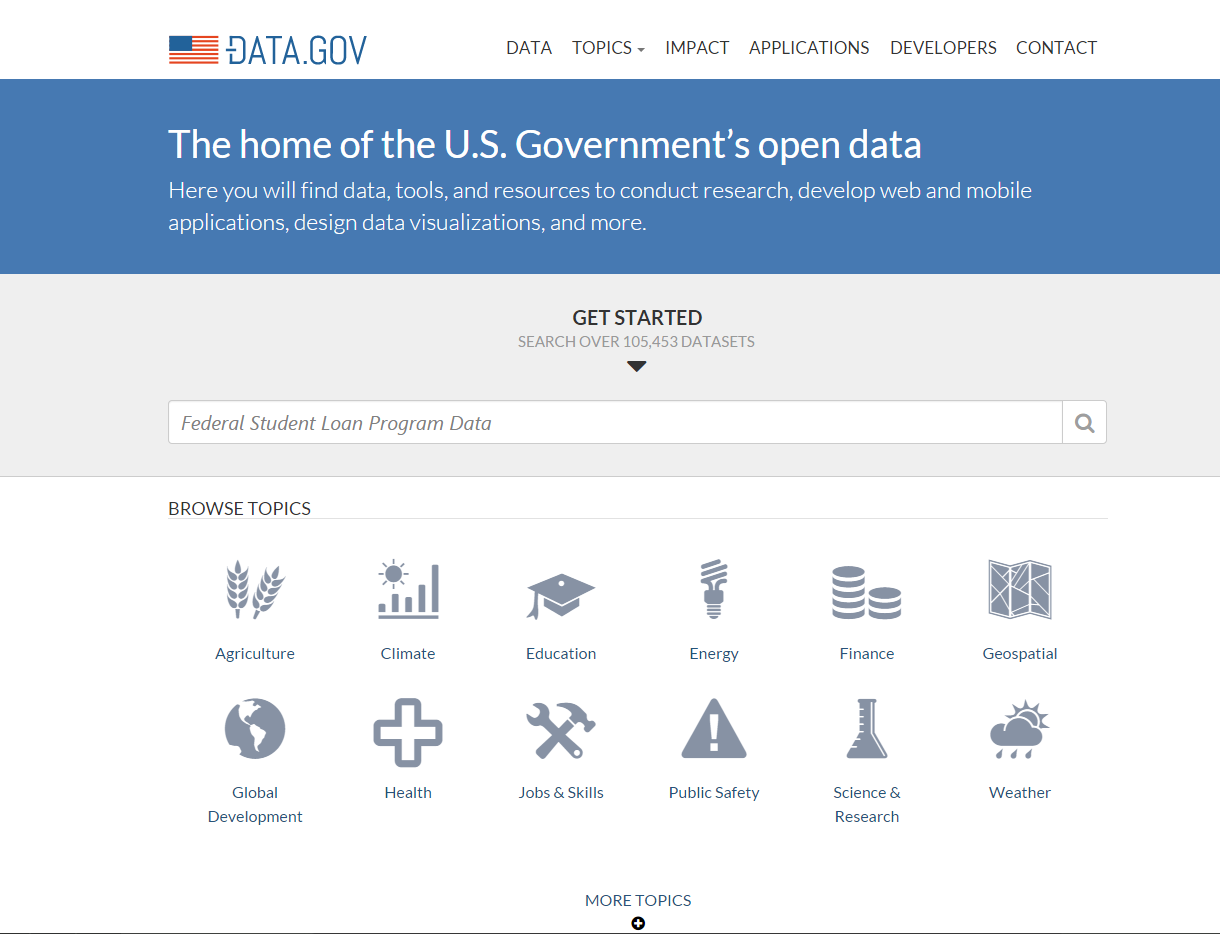
\includegraphics[width=\textwidth]{estado_arte/datagov}
\caption{Página principal del portal de datos del Gobierno de Estados Unidos}
\end{figure}

El portal utiliza CKAN \footnote{http://ckan.org/} para almacenar todos los conjuntos de datos y Drupal\footnote{https://drupal.org/} como gestor de contenidos.

Un apartado en el que el nuevo Land Portal intenta mejorar a éste portal es la visualización de datos. El nuevo Land Portal ofrecerá visualizaciones destinadas a facilitar la interpretación de los datos por parte de los usuarios.

\subsection{Portal de datos del Gobierno Británico}
El portal de datos del Gobierno Británico\footnote{http://data.gov.uk/}, al igual que el portal de datos del Gobierno de Estados Unidos, es también uno de los referentes mundiales en cuanto a portales de datos abiertos.

El portal se hizo público en enero de 2010 y actualmente contiene más de 9000 conjuntos de datos procedentes de varios departamentos del Gobierno.  Todos los conjuntos de datos se encuentran disponibles de forma gratuita para uso privado y comercial siempre que se atribuya su creación al Gobierno Británico.
\begin{figure}[h]
\centering
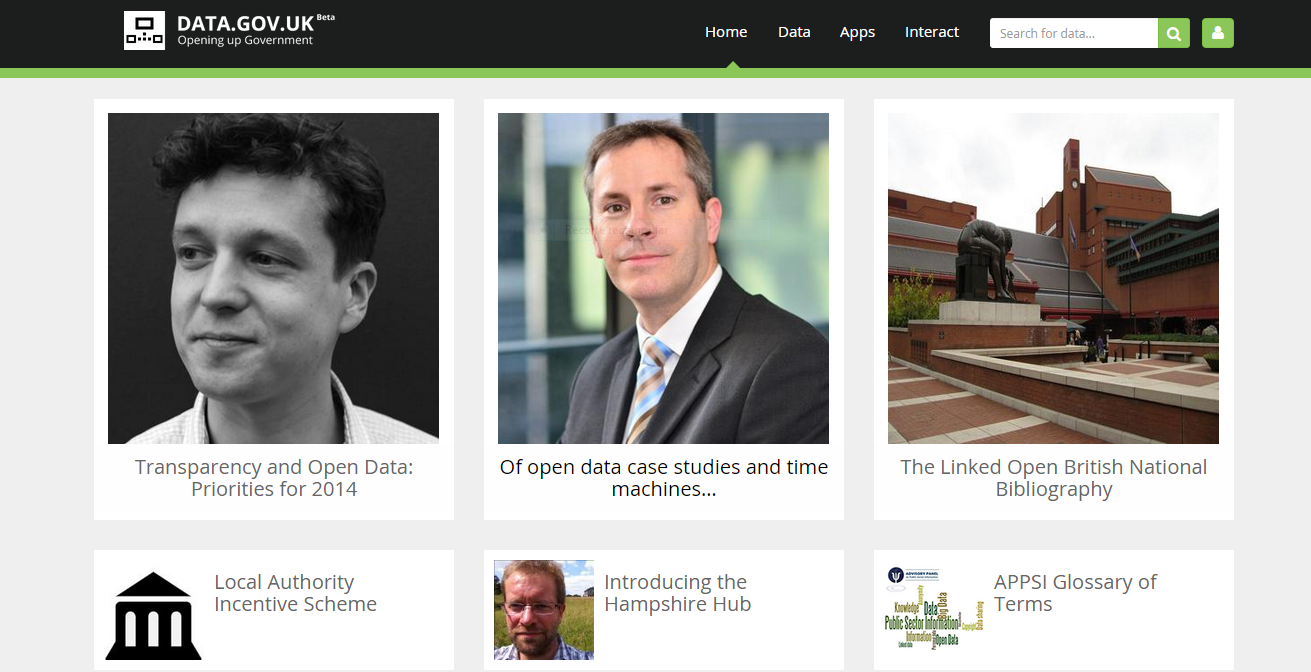
\includegraphics[width=\textwidth]{estado_arte/datagovuk}
\caption{Página principal del portal de datos del Gobierno Británico}
\end{figure}

Al igual que el portal de datos del Gobierno de Estados Unidos, este portal también utiliza CKAN y Drupal como gestor de datos y de contenido respectivamente.  Como se explicará posteriormente en esta misma sección, el nuevo Land Portal también utiliza un sistema similar, debido a su probada estabilidad en sistemas similares.  El aspecto del nuevo Land portal también se ha inspirado en el diseño claro y simple de éste portal.

\subsection{Antiguo Land Portal}
El Land Portal\footnote{http://landportal.info/} pertenece al Fondo Internacional para
el Desarrollo Agrícola, que forma parte de la ONU.  Fue creado en marzo de 2011 y actualmente cuenta con casi 1000 usuarios registrados y un total de 70 organizaciones diferentes. En el año 2012 el portal tuvo unos 70000 visitantes únicos, con cerca de 10000 visitas mensuales\footnote{Ésta información puede consultarse en \cite[página 3]{landportal-strategy}}.
\begin{figure}[h]
\centering
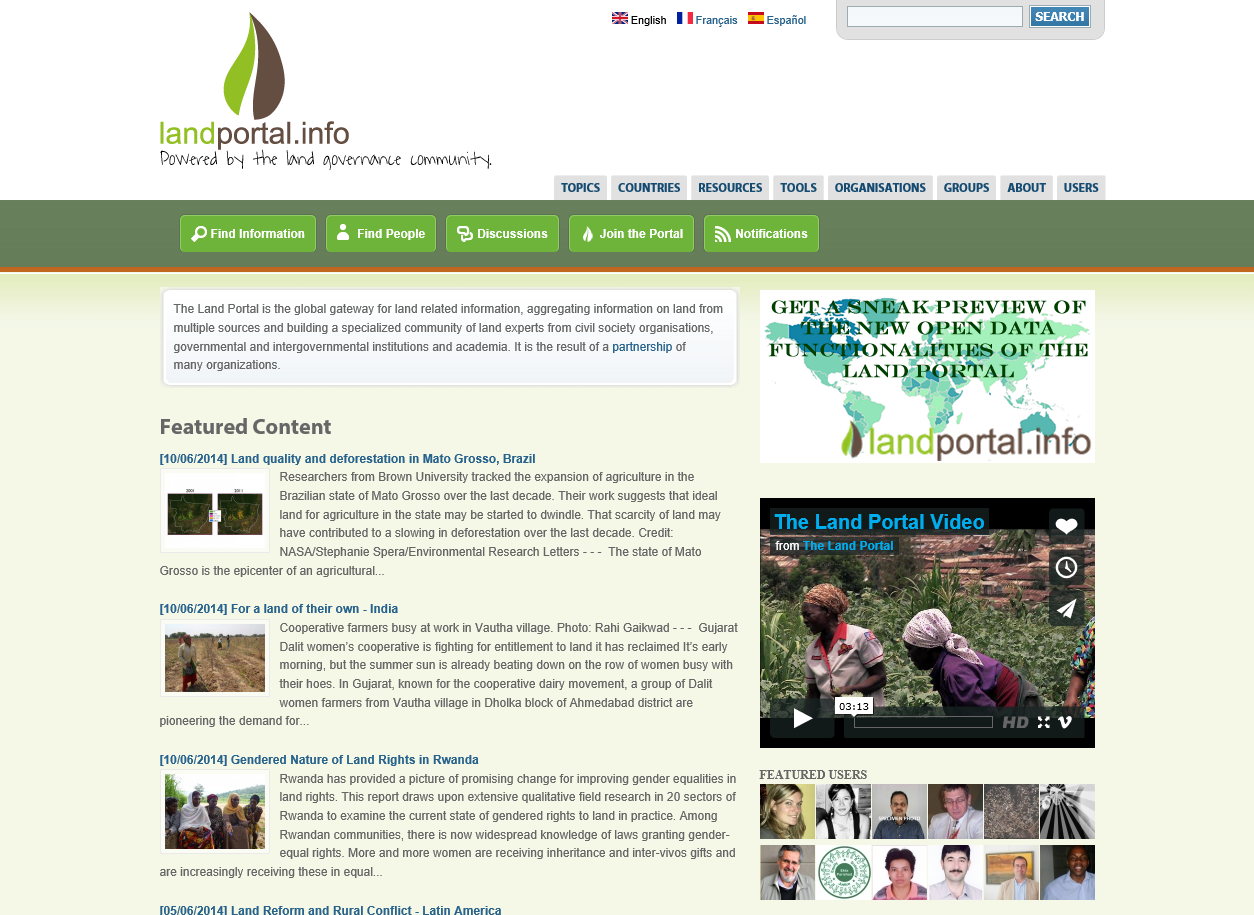
\includegraphics[width=\textwidth]{estado_arte/old_landportal_home}
\caption{Página principal del antiguo Land Portal}
\end{figure}

A pesar de no ser un portal de datos abiertos como tal, el viejo Land Portal ha sido la principal inspiración a la hora de realizar este proyecto. El nuevo portal pretende reunir y mejorar las características de los portales de datos del Gobierno Británico y del Gobierno de Estados Unidos y, al mismo tiempo, mantener el espíritu original de colaboración e intercambio de conocimientos del viejo Land Portal.  Los principales puntos en los que este proyecto pretende mejorar lo ofrecido por el viejo Land Portal son los siguientes:
\begin{itemize}
\item Ofrecer una interfaz más amigable, en línea con la sencillez y vistosidad de los portales de datos del Gobierno Británico y el Gobierno de Estados Unidos.
\item Ofrecer acceso a los conjuntos de datos procedentes de diferentes organizaciones, tanto de forma visual como a través de un API para desarrolladores y un catálogo de datos con capacidad de negociación de contenido.
\item Fomentar la participación de todos los miembros de la comunidad aportando nueva información y debatiendo sobre la ya existente.
\end{itemize}



\chapter{Evaluación de alternativas}
\label{chapter02}
\section{Alternativas evaluadas}

\subsection{Gestor de contenidos}
Un gestor de contenidos (\textit{CMS}) permite publicar, editar y modificar de forma sencilla los contenidos de una página web.  La mayoría de gestores de contenidos también se encargan de la gestión de los usuarios, los roles de usuario y permisos de cada uno de ellos.

Hay multitud de gestores de contenido disponibles en el mercado. En esta sección se van a analizarán varios de ellos y posteriormente se explicará cual se ha escogido para su utilización en éste proyecto.


\subsubsection{Joomla}
Joomla\footnote{http://www.joomla.org/} es un gestor de contenido de código abierto, con licencia GPL y escrito en PHP.  Fue creado en 2005 como un fork de otro gestor de contenido llamado \textit{Mambo}\footnote{http://www.mamboserver.com/}.\\
Joomla es utilizado en sitios web de gran relevancia, como la página web de la Universidad de Harvard\footnote{http://gsas.harvard.edu/}.

\begin{figure}[h]
\centering

\includegraphics[height=2.5cm]{joomla_logo.PNG}
\caption{Logotipo de Joomla}
\end{figure}

Las principales ventajas de Joomla respecto a otros gestores de contenido son su sencillez y su capacidad de extensión.\\
Joomla está diseñado utilizando técnicas de programación orientada a objetos y aplicando varios patrones de diseño de software, lo que hace que su código esté relativamente bien formado.\\
Por otra parte Joomla soporta cinco tipos diferentes de extensiones (componentes, plugins, plantillas, módulos e idiomas).  Cada uno de estos tipos de extensión tiene un comportamiento y una finalidad diferente, lo que permite que sea posible adaptar el funcionamiento del gestor de contenidos a cada necesidad particular.


\subsubsection{Wordpress}
Wordpress\footnote{https://wordpress.org/} es un gestor de contenido de código abierto, con licencia GLPv2 y escrito en PHP.  Fue creado en mayo de 2003 como un fork de otro gestor de contenido llamado \textit{b2/cafelog}.\\
En la actualidad Wordpress se utiliza en más de 68 millones de sitios web, entre ellos el sitio web del New York Times\footnote{http://www.nytimes.com/}, el sitio web de CNN\footnote{http://edition.cnn.com/} o el sitio web de Forbes\footnote{http://www.forbes.com/}.

\begin{figure}[h]
\centering

\includegraphics[height=2.5cm]{wordpress_logo.PNG}
\caption{Logotipo de Wordpress}
\end{figure}

La principal ventaja de Wordpress respecto a otros gestores de contendo es su simplicidad, puesto que está orientado principalmente a la construcción de sitios orientados al blogging o a las noticias.


\subsubsection{Drupal}
Drupal\footnote{https://drupal.org/} es un gestor de contenido de código abierto creado en el año 2001.  Al igual que Joomla y Wordpress está escrito en PHP y cuenta con licencia GPLv2.\\
Como se ha mencionado anteriormente, Drupal se utiliza en el portal de datos del Gobierno Británico\footnote{http://data.gov.uk/} y en el portal de datos del Gobierno de Estados Unidos\footnote{http://www.data.gov/}.

\begin{figure}[h]
\centering

\includegraphics[height=2.5cm]{drupal_logo.PNG}
\caption{Logotipo de Drupal}
\end{figure}

La principal ventaja de Drupal es su flexibilidad para extender y modificar su funcionamiento.  En la actualidad cuenta con más de 15000 módulos disponibles.  Su sistema de \textit{hooks} permite crear módulos que son llamados y ejecutados de forma automática por el \textit{core} de Drupal.





\subsection{Catálogo de datos}
Un catálogo de datos permite almacenar y organizar bajo una estructura común catálogos de datos procedentes de diversas fuentes y que pueden encontrarse en distintos formatos.


\subsubsection{CKAN}
CKAN\footnote{http://ckan.org/} (\textit{Comprehensive Knowledge Archive Network}) es una plataforma de código abierto para la construcción de portales de datos y creada por la OKFN (\textit{Open Knowledge Foundation})\footnote{https://okfn.org/} que permite publicar, buscar y organizar catálogos de datos. CKAN está escrito en Python\footnote{https://www.python.org/} y utiliza PostgreSQL\footnote{http://www.postgresql.org/} como base de datos.

El funcionamiento de CKAN consiste en almacenar los catálogos de datos junto con diversos metadatos, que posteriormente son accesibles y modificables desde una interfaz web amigable para los usuarios.  Además de la interfaz web CKAN también ofrece una API que permite interactuar con otras aplicaciones y servicios.

Como se ha mencionado anteriormente, CKAN se utiliza en varios portales de datos de gran envergadura, como pueden ser el portal de datos del Gobierno Británico o el portal de datos del Gobierno de Estados Unidos.


\subsubsection{DKAN}
DKAN\footnote{http://nucivic.com/dkan/} es una plataforma basada en CKAN y Drupal para facilitar la publicación de datos.  A diferencia de CKAN, DKAN está escrito utilizando el lenguaje de programación PHP.

La principal ventaja de DKAN es la estrecha integración entre el catálogo de datos (CKAN) y el gestor de contenidos (Drupal).  Ésta integración entre los dos componentes permite aprovechar las mejores características de cada uno de ellos.  Por otra parte, ésta integración también permite desplegar el catálogo de datos de una forma simple sobre una instalación de Drupal ya existente.

Un punto en contra de DKAN es su falta de madurez.  DKAN fue creado en 2012 y recientemente ha alcanzado la versión 1.0.  A pesar de todo, ha sido utilizado en algunos proyectos como el portal de datos de la ciudad de Colonia y el portal de datos del Gobierno de Puerto Rico.


\subsubsection{Herramienta creada especialmente para la ocasión}
La funcionalidad de un catálogo de datos podría ser implementada por una herramienta creada especialmente para éste proyecto e implementada como un módulo del gestor de contenidos.

La principal ventaja de esta aproximación es que, dado que la herramienta se crearía especialmente para éste proyecto, cumpliría totalmente con las necesidades del mismo.  La principal desventaja radica en el esfuerzo requerido para implementar una herramienta de tal calibre, esfuerzo que ya viene solucionado por parte una herramienta como DKAN.



\subsection{Servidor semántico}
Puesto que éste proyecto consiste en la creación de un portal de datos enlazados abiertos, es necesario incluir un componente que se encargue de aportar la parte de datos enlazados.  Éstos componentes suelen llamarse servidores semánticos o \textit{triple-stores}, puesto que almacenan los datos en formato RDF\footnote{http://www.w3.org/RDF/}, que modela los datos en forma de tripletas.


\subsubsection{Virtuoso Universal Server / Virtuoso OpenLink}
Virtuoso Universal Server\footnote{http://virtuoso.openlinksw.com/} es un motor de base de datos con una arquitectura híbrida que le permite ofrecer diferentes funcionalidades, que tradicionalmente han sido realizadas por diferentes productos, en un mismo componente.\\
Virtuoso fue creado en 1998 de la unión del middleware de acceso a datos \textit{OpenLink}  y el sistema de gestión de bases de datos relacionales \textit{Kubl}.

Además de la capacidad para ofrecer diferentes servicios en un mismo componente, otra gran ventaja de Virtuoso es su estabilidad y rendimiento.  
Las principales ventajas de Virtuoso son su capacidad para ofrecer diferentes servicios desde un mismo componente y su estabilidad y rendimiento. Además Virtuoso porporciona un punto de acceso SPARQL\footnote{SPARQL es un lenguaje para realizar consultas en grafos RDF de forma similar a cómo SQL sirve para realizar consultas en bases de datos relacionales.} para consultar los datos que almacena.\\
Como se indica en \cite[]{largetriplestores}, la versión 6.1 de Virtuoso ha llegado a servir 15.4 billones de tripletas simultáneamente (incluyendo el catálogo completo del portal de datos del Gobierno de Estados Unidos).

Virtuoso un producto propietario, aunque tiene una versión libre con licencia GLPLv2 que recibe el nombre de Virtuoso OpenLink\footnote{http://virtuoso.openlinksw.com/dataspace/doc/dav/wiki/Main/}. Virtuoso y Virtuoso OpenLink es utilizado activamente en varios portales de datos, entre ellos el portal de datos de la Web Foundation\footnote{http://data.webfoundation.org/} y la DBPedia\footnote{http://wiki.dbpedia.org/}.


\subsubsection{Stardog}
Stardog\footnote{http://www.stardog.com/} es un sistema de base de datos RDF escrit en Java. Stardog es un producto comercial, aunque cuenta con una versión gratuita con características limitadas.

La principal ventaja de Stardog frente al resto de servidores semánticos es su capacidad para realizar inferencias sobre los datos que almacena, así como su soporte a la especificación OWL2\footnote{OWL2 es un estándar publicado en 2008 por el W3C con el objetivo de construir un modelo de marcas basado en RDF y codificado en XML.}.

Como se menciona en \cite[]{largetriplestores}, la versión 2.1 de Stardog soporta hasta 50 billones de tripletas almacenadas simultáneamente.


\subsubsection{4store}
4store\footnote{http://4store.org/} es un sistema de gestión de bases de datos y un motor de consultas que almacena datos en formato RDF. 4store está escrito en ANSI C99 y cuenta con licencia GPLv3.

Las principales ventajas de 4store son su rendimiento, su escalabilidad y su estabilidad. 4store lleva siendo usado en producción en Garlik\footnote{http://www.garlik.com/} durante 3 años. Como se puede ver en \cite[]{largetriplestores}, 4store soporta hasta 15 billones de tripletas almacenadas simultáneamente.
Por otra parte, una posible desventaja de 4store es el número de características que ofrece. 4store únicamente proporciona almacenamiento RDF y consultas SPARQL.



\subsection{Visualizador de datos enlazados}
Un visualizador de datos enlazados accede a los datos que se almacenan en el servidor semántico en formato RDF para mostrarlos de una forma que atractiva para el usuario y permitir navegar a través de ellos sin necesidad de realizar complejas consultas SPARQL.


\subsubsection{Pubby}
Pubby\footnote{http://wifo5-03.informatik.uni-mannheim.de/pubby/} es un visualizador de datos enlazados escrito en Java.  Pubby fue creado por Richard Cyganiak y cuenta con una licencia Apache v2.

La principal ventaja de Pubby es su facilidad de configuración y su demostrada estabilidad. Tal y como Chris Bizer explica en \citation[Architectural Evolution]{dbpedia-architecture} Pubby fue utilizado como frontend de Virtuoso en DBPedia antes de ser sustituido por consumidores especializados en HTML y RDF por cuestiones de rendimiento.

La principal desventaja de Pubby es su estado de abandono. Al momento de realizar éste proyecto, la última actualización de Pubby data de enero de 2011.

\subsubsection{Wesby}
Wesby\footnote{https://github.com/weso/wesby} es un visualizador de datos enlazados escrito en Scala. Es un desarrollo propio de WESO\footnote{http://www.weso.es/} que tiene como objetivo ser una alternativa que mejore lo ofrecido por Pubby.

\begin{figure}[h]
\centering
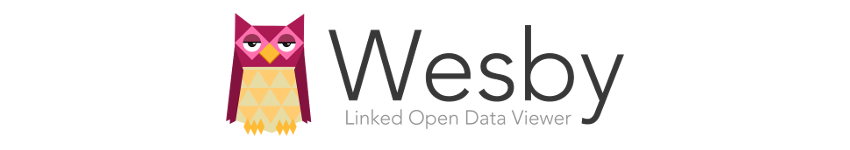
\includegraphics[width=\textwidth]{wesby_logo.PNG}
\caption{Logotipo de Wesby}
\end{figure}

La principal ventaja de Wesby sobre Pubby es su apariencia. Wesby ofrece una interfaz limpia y adaptable a diferentes dispositivos. Además, una caracerística ofrecida por Wesby es el soporte para la creación de visualizaciones para diferentes tipos de nodos dentro del grafo RDF. Otra ventaja de Wesby es que éste construye automáticamente el esquema de URIs a partir del grafo de datos presente en el servidor semántico al que se conecta.

Una posible desventaja de Wesby respecto a Pubby es su novedad. Wesby es un proyecto relativamente nuevo, y únicamente se ha utilizado en el portal de datos de la Web Foundation.



\subsection{Framework de diseño web}
Un framework de diseño web facilita la tarea de diseñar la interfaz de la web de forma que resulte atractiva a los usuarios.


\subsubsection{Twitter Bootstrap}
Bootstrap\footnote{http://getbootstrap.com/} es un framework de diseño web desarrollado por Mark Otto y Jacob Thornton y vió la luz como proyecto de código abierto en el año 2011.

Una gran ventaja de Bootstrap respecto a otros frameworks de diseño web es el gran número de elementos prediseñados con el que cuenta. Otra característica interesante de Bootstrap es que facilita el desarrollo adaptable a diferentes dispositivos al utilizar una organización en filas y columnas de ancho variable.\\
Bootstrap es utilizado en multitud de sitios web, por lo que cuenta con una comunidad muy amplia y existe una gran cantidad de temas y documentación disponible.

Una desventaja de Bootstrap y, en general, de cualquier framework de diseño web es que obliga a realizar el desarrollo de una forma determinada.


\subsubsection{ZURB Foundation}
Foundation\footnote{http://foundation.zurb.com/} es un framework de diseño web desarrollado por ZURB en 2011.

La principal ventaja de Foundation respecto a otros frameworks de diseño web es que permite diseñar la web orientada principalmente a dispositivos móviles y adaptada a pantallas de un tamaño más grande.

Una característica de Foundation que produce al mismo tiempo ventajas y desventajas es que Foundation cuenta con menos elementos prediseñados, algo que obliga al desarrollador trabajar más pero, al mismo tiempo, permite una mayor flexibilidad en los diseños.


\subsubsection{Desarrollo desde cero}
Una tercera alternativa es realizar el diseño del portal desde cero sin utilizar ningún framework.

La principal ventaja de esta solución es la total flexibilidad para desarrollar y dar la apariencia que se desee sin estar sujetos a las ataduras de un framework.

La principal desventaja es la cantidad de trabajo necesario para implementar y mantener una apariencia coherente a lo largo de todo el portal, además de el esfuerzo necesario para conseguir una interfaz adaptable a diferentes dispositivos.



\subsection{Motor de búsqueda}
Un motor de búsqueda se encarga de catalogar e indexar los contenidos de un portal, construyendo un índice inverso que permita a los usuarios encontrar la información que necesiten.

Se han analizado dos productos de búsqueda que se detallarán a continuación.


\subsubsection{Apache Solr}
Solr\footnote{http://lucene.apache.org/solr/} es un motor de búsqueda desarrollado por la Apache Software Foundation\footnote{http://www.apache.org/foundation/}.  Fue creado en el año 2004 utilizando el lenguaje Java y tiene una licencia Apache v2. \\
Solr utiliza la librería de busqueda \textit{Lucene}\footnote{http://lucene.apache.org/}, desarrollada también por la Apache Software Foundation.  En el año 2010 los equipos de desarrollo encargados de Solr y Lucene se unieron en uno sólo, desde entonces es común referirse a ambos productos como  \textit{Lucene/Solr}.

Un punto a favor de Solr es su madurez y su amplia comunidad de usuarios y desarrolladores, lo que permite encontrar plugins para integrarlo en multitud de productos. Solr es utilizado en multitud de proyectos como Netflix\footnote{https://www.netflix.com/global}, Apple\footnote{http://www.apple.com/}, MTV\footnote{http://www.mtv.com/} o digg\footnote{http://digg.com/}. \newline
Otra característica positiva de Solr es la existencia de una API de búsqueda por HTTP. La API HTTP de Solr recibe peticiones GET y permite escoger entre varios formatos de respuesta como XML o JSON.

Un punto que puede resultar negativo de Solr frente a otros motores de búsqueda es la necesidad de definir un esquema.  El esquema es un fichero en formato XML que define qué estructura tendrá el índice.  A pesar de esto, es posible definir elementos dinámicos que se creen bajo demanda sin tener que figurar en el esquema.

\subsubsection{Elasticsearch}
Elasticsearch\footnote{http://www.elasticsearch.org/} es un motor de búsqueda desarrollado por la Organización Elasticsearch\footnote{https://github.com/elasticsearch}.  Fue creado en 2010 por Shay Banon utilizando el lenguaje Java.  Al igual que Solr, Elasticsearch también cuenta con una licencia Apache v2 y utiliza la librería de búsqueda Lucene.

La principales características a favor de Elasticsearch son su capacidad para construir sistemas de búsqueda distribuidos y su arquitectura \textit{schemaless}, lo que permite enviar documentos para que sean indexados sin necesidad de definir un esquema previamente.

El punto débil de Elasticsearch es su novedad. A pesar de ser utilizado en portales como Quora\footnote{https://www.quora.com/} o GitHub\footnote{https://github.com/} no cuenta con la madurez y amplia comunidad de productos más maduros como Solr.


\subsubsection{Buscador propio del gestor de contenidos}
Los tres gestores de contenidos que se han analizado anteriormente cuentan con un buscador propio integrado.  La principal ventaja de éste buscador es la completa integración con los contenidos que forman parte del CMS.  Puesto que el buscador ya forma parte del CMS, normalmente no es necesario realizar ninguna tarea de programación para activarlo.

La gran desventaja de ésta solución es la imposibilidad de indexar y buscar todos aquellos contenidos que no formen parte del CMS.  En éste proyecto esto haría imposible buscar los contenidos no pertenecientes a la parte social.



\section{Alternativas elegidas}
\label{chapter02:alternativas_seleccionadas}
\label{seccion_alternativas}
En esta sección se explicará qué alternativas de las anteriormente descritas se han seleccionado y las razones que han llevado a dicha selección.

\subsection{Gestor de contenidos}
De los tres gestores de contenidos analizados para éste proyecto, se ha seleccionado Drupal debido principalmente su madurez y flexibilidad.

A pesar de que los tres gestores de contenidos analizados se utilizan actualmente en multitud de proyectos, Drupal forma parte de varios proyectos con objetivos similares a éste, como los portales de datos del Gobierno Británico y del Gobierno de Estados Unidos ya mencionados anteriormente. Por otra parte, una característica a tener muy en cuenta es la cantidad de módulos disponibles para extender Drupal, que en éste momento supera los 15000.

Un punto importante en esta decisión es que, como Larry Garfield explica en \cite[]{pac-vs-mvc} Drupal utiliza el patrón arquitectónico PAC\footnote{Presentation Abstraction Control - http://en.wikipedia.org/wiki/Presentation-abstraction-control} para organizar su estructura y funcionamiento.  El patrón PAC es menos conocido y utilizado que el patrón MVC\footnote{Model View Controller - http://martinfowler.com/eaaDev/uiArchs.html}, lo que puede reflejarse en una mayor dificultad a la hora de realizar la implementación.


\subsection{Catálogo de datos}
Entre las dos alternativas mencionadas anteriormente, se ha seleccionado CKAN como catálogo de datos para éste proyecto.

Al igual que Drupal, CKAN se utiliza en varios portales de datos con objetivos similares al que se pretende construir en éste proyecto. CKAN permitirá ofrecer una vista completa de los conjuntos de datos incluidos en Land Portal.

La alternativa de utilizar una herramienta implementada especialmente para el proyecto se ha descartado por la gran complejidad que conlleva tanto la propia implementación como la integración con el gestor de conteidos y la creación de una interfaz de acceso a los datos.


\subsection{Servidor semántico}
Se ha seleccionado Virtuoso como servidor semántico para el nuevo Land Portal. Ésta seleccion viene motivada por varios factores que se explicarán a continuación.

Como se ha explicado anteriormente, Virtuoso ofrece un punto de acceso SPARQL, algo que se considera indispensable en cualquier portal de datos abiertos y enlazados.  Además, a diferencia de otras alternativas como Stardog, la versión libre de Virtuoso no tiene ninguna limitación en el número de conexiones que puede recibir ni en el uso de CPU, la única limitación de la versión libre es su capacidad para funcionar como una única instancia, pero ésto no debería ser un problema con la cantidad de datos que se pretende almacenar.

Por útlimo, al contrario que 4store, Virtuoso ofrece un API que permite almacenar y extraer datos, lo que puede resultar de utilidad a la hora de realizar el proceso de importación y enriquecimiento de datos.


\subsection{Visualizador de datos enlazados}
Entre las dos alternativas para el visualizador de datos enlazados se ha seleccionado Wesby.

Ésta selección viene motivada principalmente por ser Wesby un desarrollo propio del grupo de investigación WESO en el que yo mismo he participado, además de por ofrecer una interfaz moderna, amigable y adaptable a diferentes dispositivos que permitirá que no desentone respecto a las demás partes del nuevo Land Portal.


\subsection{Framework de diseño web}
Como framework de diseño web se ha seleccionado Bootstrap.

La principal razón para seleccionar Bootstrap frente a Foundation es que Bootstrap cuenta con una mayor cantidad de usuarios, lo que produce una mayor comunidad y permite encontrar recursos como documentación, temas, etc. más fácilmente.

El desarrollo de la apariencia del portal sin utilizar un framework de diseño web ha sido descartado debido al gran esfuerzo que requeriría en implementar un diseño moderno, vistoso, coherente y adaptativo desde cero.


\subsection{Motor de búsqueda}
La decisión del motor de búsqueda ha sido quizás de las más complejas. La decisión final ha sido en favor de Solr.

A pesar de que tanto Solr como Elasticsearch son utilizados en varios proyectos importantes, la mayor madurez de Solr hace más sencillo encontrar plugins e información.  En relación con la decisión del gestor de contenido, Solr cuenta con un plugin para Drupal\footnote{https://drupal.org/project/apachesolr} que lleva 7 años en desarrollo activo, por lo que su madurez y estabilidad quedan fuera de toda duda.

Debido también a la cantidad de datos con la que contará el portal tampoco parece necesario recurrir a las altas capacidades de búsqueda distribuida ofrecidas por Elasticsearch.



\chapter{Conceptos teóricos}
\label{chapter03}
En éste capítulo se definirán los conceptos teóricos necesarios para comprender correctamente la finalidad del sistema en construcción.

\section{Datos abiertos}
El concepto de datos abiertos u \textit{Open Data} es definido por la Open Knowledge Foundation en \cite{opendefinition} de la siguiente forma:
\begin{quote}
\textit{``A piece of data or content is open if anyone is free to use, reuse, and redistribute it — subject only, at most, to the requirement to attribute and/or share-alike.''}
\end{quote}

De la anterior definición pueden destacarse tres pilares fundamentales que marcan la diferencia entre los datos abiertos y el resto de datos, dichos puntos clave se explicarán a continuación:
\begin{itemize}
\item Acceso y disponibilidad. Los datos deben estar disponibles en su totalidad con un coste razonable o, preferiblemente, de forma gratuita a través de Internet.  Es también importante que el formato en el que se publican los datos sea conveniente y modificable.
\item Reutilización y redistribución.  La licencia bajo la que se publican los datos no debe restringir la redistribución de los mismos ni exigir pagos o cuotas por dicha redistribución.  Además, la licencia debe permitir modificar los datos e incluso cruzarlos con datos provenientes de otras fuentes.
\item Participación universal.  Los datos no deben poner trabas para ser accedidos por ninguna persona ni grupo de personas ni deben restringir el uso de los mismos a un ámbito de trabajo específico.
\end{itemize}

Cualquier conjunto de datos puede ser considerado un conjunto de datos abiertos si cumple con la definicion anterior, aunque las principales fuentes de datos abiertos generalmente provienen de fuentes científicas o gubernamentales.  En el año 2004 los ministros de ciencia de todas las naciones pertenecientes a la OECD\footnote{La OECD (Organización para la Cooperación y el Desarrollo Económico) es una de las organizaciones que aporta los conjuntos de datos con los que se trabaja en éste proyecto.} firmaron una declaración en la que se aboga por hacer públicos toda la información científica financiada con fondos públicos.

En cuanto a los datos abiertos procedentes de fuentes gubernamentales, como ya se ha mencionado en el capítulo \ref{chapter01} - \nameref{chapter01}, la tendencia de los gobiernos de ofrecer datos en forma abierta es cada vez mayor tal y como evidencian los múltiples portales de datos propiedad de la administración pública que han surgido recientemente. Algunos ejemplos son: el portal de datos del Gobierno de España\footnote{http://datos.gob.es/}, el portal de datos del Gobierno de Reino Unido\footnote{http://data.gov.uk/} o el portal de datos del Gobierno de Estados Unidos\footnote{http://www.data.gov/}.



\section{Datos enlazados}
El concepto de datos enlazados o \textit{Linked Data} fue acuñado por Tim Berners-Lee, director del W3C\footnote{World Wide Web Consortium}, y describe un método de publicar catálogos datos estructurados de una forma en la que sea posible conectarlos con otros catálogos de datos procedentes de diferentes fuentes.

En \cite{tbl-linkedopendata}, Tim Berners-Lee define los cuatro elementos fundamentales para los datos enlazados:
\begin{itemize}
\item Usar URIs para nombrar los elementos.
\item Usar URIs HTTP para permitir a las personas acceder y buscar dichos nombres.
\item Cuando alguien accede a una URI, devolver la información de forma útil usando los estándares RDF o SPARQL.
\item Incluir enlaces a otras URIs para facilitar el descubrimiento de más elementos.
\end{itemize}



\section{Datos enlazados abiertos}
El concepto de datos enlazados abiertos (\textit{Linked Open Data}) combina los conceptos de datos abiertos (\textit{Open Data}) y datos enlazados (\textit{Linked Data}) que se han explicado en las secciones anteriores.

Un conjunto de datos se considera un conjunto de datos enlazados abiertos si cumple los requisitos de los datos enlazados y además se presenta bajo una licencia abierta que no impida su reutilización ni redistribución.


\subsection{Sistema de estrellas}
Como se menciona en \cite{tbl-linkedopendata}, en el año 2010 Tim Berners-Lee desarrolló un sistema de estrellas o niveles con el objetivo de concienciar (principalmente a las organizaciones gubernamentales) en el uso de datos enlazados abiertos.

A continuación se explica el significado de cada nivel de esta escala:
\begin{enumerate}
    \item Los datos están disponibles en cualquier formato (pero manteniendo una licencia libre para ser considerados datos abiertos).  Un ejemplo serían datos publicados como una imagen escaneada.
    \item Los datos se encuentran en un formato estructurado y que pueda ser leído por máquinas.  Por ejemplo utilizar un formato \textit{Microsoft Excel} en lugar de una imagen escaneada.
    \item Similar al anterior pero utilizando un formato libre, por ejemplo CSV, JSON o XML.
    \item Cumple con todos los niveles anteriores pero además utiliza un estándar abierto de la W3C como RDF o SPARQL.  El uso de estos estándares permite que el catálogo de datos sea enlazado por otros catálogos u organizaciones.
    \item Cumple con todos los niveles anteriores, pero además enlaza hacia otros catálogos de datos externos.
\end{enumerate}

El portal de datos que se pretende construir en éste proyecto pretende cumplir con un nivel de 5 estrellas.



\section{RDF Data Cube}
\label{concept:rdf_data_cube}
En la especificación del RDF Data Cube Vocabulary (recomendación de enero de 2014) \cite{w3c:data-cube} se define el objetivo de éste vocabulario de la siguiente forma:
\begin{quote}
\textit{``There are many situations where it would be useful to be able to publish multi-dimensional data, such as statistics, on the web in such a way that it can be linked to related data sets and concepts. The Data Cube vocabulary provides a means to do this using the W3C RDF (Resource Description Framework) standard [...]''}
\end{quote}

Puesto que uno de los objetivos del portal que se construirá en éste proyecto es precisamente la publicación de datos multidimensionales en la web, la estructura del modelo de datos intentará adecuarse a la estructura descrita por el RDF Data Cube Vocabulary.  El diseño del modelo de datos puede ser visto de forma detallada en la sección SECCIÓN DEL MODELO DE DATOS.

A modo de resumen, el RDF Data Cube pretende definir una estructura y un vocabulario basado en el estándar RDF con el que publicar conjuntos de datos multidimensionales en la web.  Los conjuntos de datos son colecciones de datos con una estructura determinada.  Los datos contenidos conjunto de datos serán de alguno de los siguientes tipos:
\begin{description}
\item[Observaciones]  Es la información final a la que se quiere acceder, los valores de las mediciones o los cálculos realizados.
\item[Información organizativa]  Ayuda a encontrar una cierta observación o un conjunto de observaciones.  Para encontrar una observación será necesario conocer las dimensiones bajo las que se encuentra.
\item[Información estructural]   Ayuda a interpretar una cierta observación, por ejemplo indicando su unidad de medida o si es un valor exacto o estimado.
\item[Metadatos del conjunto de datos]  Ayudan a describir información sobre el propio conjunto de datos, por ejemplo su publicador.
\end{description}

\subsection{El modelo de cubo}
El RDF Data Cube Vocabulary pretende crear el concepto de cubo o \textit{hypercube} como forma de representar la estructura de la información. El cubo en el que se encuentran las observaciones se organiza en torno a un conjunto de dimensiones, atributos y medidas (todos ellos reciben el nombre de \textit{componentes}).
\begin{description}
\item[Dimensiones]  Permiten localizar una observación concreta o un conjunto de observaciones.  Por ejemplo una dimensión podría ser la zona geográfica sobre la que las observaciones han tenido lugar o el momento en el tiempo al que las observaciones hacen referencia.
\item[Medidas]  Representan el fenómeno concreto observado.
\item[Atributos]  Permiten realizar cuantificar e interpretar los valores observados.  Por ejemplo un atributo podría ser la unidad de medida de una observación.
\end{description}

\subsection{Los \textit{slices}}
El concepto de \textit{slice} hace referencia a un subconjunto o agrupación de las observaciones existentes en el cubo.

Por ejemplo, usando los datos reales con los que se trabajará en el portal que se pretende construir en éste proyecto, dadas una serie de observaciones tomadas para diversos indicadores y países a lo largo de un periodo de tiempo, podría ser interesante agrupar dichas observaciones según su indicador y el momento de tiempo en el que se han realizado.  Cada uno de estos grupos representaría todas las observaciones de todos los países para un determinado indicador y momento temporal.  Éstos grupos reciben el nombre de \textit{slices}.



\chapter{Análisis}
\label{chapter04}
\section{Definición del sistema}
\label{definicion_sistema}
Tal y como se ha mencionado en el capítulo de \nameref{chapter01}, éste proyecto se encuadra dentro del proyecto \textit{Rebuilding IFAD's LandPortal RFQ/2013/016/SC} desarrollado por el grupo de investigación WESO y la empresa SB Consulting. El cliente a quien va destinado es Fondo Internacional para el Desarrollo Agrícola, que forma parte de la Organización de las Naciones Unidas.
Conviene definir en este momento una terminología común que se va a utilizar de ahora en adelante.  Se hablará de \textit{sistema} para hacer referencia al nuevo Land Portal en su totalidad, por otra parte se hablará de \textit{proyecto} para hacer referencia al backend del nuevo Land Portal del que es objeto la presente documentación.


\subsection{Alcance del sistema}
A continuación se explicará qué partes del desarrollo del nuevo Land Portal tienen cabida en éste proyecto.  También se mencionarán las partes que no entrarán dentro del alcance del proyecto para que el lector pueda apreciar la complejidad del sistema en su totalidad.

\subsubsection{Elementos dentro del alcance del proyecto}
\begin{itemize}
\item Punto de entrada único para los datos del portal.  Como se ha explicado anteriormente los datos del portal procederán de diversas fuentes de datos y organizaciones externas.  Con el fin de mantener el control sobre el tiempo y forma en la que se incluyen nuevos datos será necesario crear un punto único de entrada para los mismos.  Para garantizar una cierta uniformidad y asegurar un nivel de calidad mínimo también será necesario definir un formato en el que enviar los datos hacia éste punto de entrada.\newline
Por otra parte, un componente como éste tiene una gran responsabilidad en el correcto funcionamiento del portal, por lo que será necesario establecer unas medidas de seguridad que eviten la introducción de datos procedentes de orígenes no confiables.\newline
Además será necesario insertar en una base de datos relacional los datos que lleguen al punto de entrada.  Los datos que se almacenen en ésta base de datos se utilizarán para la construcción del framework que da soporte a las visualizaciones de datos y que se verá a continuación.
\item Framework para proveer información con la que construir visualizaciones de datos.  Éste portal de datos no se limitará a almacenar y devolver catálogos de datos, si no que también ofrecerá visualizaciones que permitan a los usuarios acceder los datos de una forma sencilla y atractiva.  Como parte del proyecto se desarrollará un framework que permita proveer la información necesaria para construir las visualizaciones de datos.
\item Arquitectura para la creación de vistas personalizadas.  Además de la creación de un framework que provee la información necesaria para construir visualizaciones de datos también será necesario la creación de una arquitectura que permita incluir vistas personalizadas   Con el fin de hacer ésta arquitectura lo más general y reutilizable posible se evitará hacer uso de los mecanismos que el CMS provee para la creación de vistas.
\item Mecanismo de internacionalización.  Puesto que éste portal ofrecerá datos procedentes de diversas organizaciones internacionales y relativos a multitud de países y continentes distintos será necesario proveer un mecanismo de internacionalización que permita a los usuarios acceder a la información en el lenguaje que prefieran.  Además será necesario que el mecanismo de internacionalización no se limite simplemente a soportar traducciones para la información estática, si no que tendrá que ir más allá y permitir la internacionalización de los propios datos.
\item Plataforma social que fomente la participación de los usuarios y complemente la información de los conjuntos de datos.  Puesto que el nuevo Land Portal pretende hacer especial énfasis en la participación de los usuarios será necesario ofrecer una plataforma en la que la comunidad pueda interactuar e intercambiar información.  Bajo dicha plataforma se crearán debates para que los usuarios intercambien sus opiniones a cerca de algún tema concreto, noticias para mantener al resto de usuarios informados sobre aquellas informaciones que se consideren necesarias y eventos que tendrán lugar en una fecha concreta.  Además también albergará un blog en el que el propio Land Portal coloque aquella información que considere relevante para sus usuarios.\newline
Dado que ésta plataforma estará completamente integrada dentro del nuevo Land Portal será también necesario que cuente con un aspecto uniforme y que mantenga la línea de identidad del portal, de forma que la transición entre las diferentes partes sea transparente al usuario.  Las vistas realizadas para ésta parte del portal utilizarán los propios mecanismos ofrecidos por el CMS para la creación de vistas y plantillas visuales. 
\item Componente de autenticación de los usuarios para usar el API.  Como se verá posteriormente la implementación del API del nuevo Land Portal queda fuera del alcance de éste proyecto, aunque sí que será necesario implementar un componente que permita controlar las claves de acceso al API.  La seguridad del API es un apartado muy importante, por lo que sólo deberán tener acceso aquellos usuarios que la administración desee.  En relación con el punto anterior, la generación de las claves de acceso deberá realizarse de forma transparente al usuario.
\item Unificación de la búsqueda entre las diferentes partes del portal.  Con el fin de centralizar la búsqueda en una única parte del portal, será necesario unificar la búsqueda de la parte social perteneciente al CMS y de la parte de datos, cuyos datos se encuentran almacenados fuera del CMS.
\end{itemize}

\subsubsection{Elementos fuera del alcance del proyecto}
\begin{itemize}
\item Generación de RDF y enriquecimiento de datos.  Como se ha explicado anteriormente uno de los objetivos de éste proyecto es diseñar un punto de entrada único para los datos del portal, además de implementar un mecanismo que inserte dichos datos en una base de datos relacional.  Un elemento fuera del alcance de éste proyecto, pero que sí se encuentra dentro del sistema real es un componente encargado de la generación de datos en formato RDF y el enriquecimiento de los mismos.  Además dicho componente también almacenará los datos en Virtuoso, que fue escogido como servidor semántico tal y como se mencionó en la sección ``\nameref{seccion_alternativas}'' del capítulo \ref{chapter02}.
\item Importación de datos.  Siendo el sistema que se pretende construir un portal de datos, la importación de los propios datos juega un papel clave en la buena marcha del mismo.  Tal y como ya se ha explicado en la sección ``\nameref{objetivos_proyecto}'' perteneciente al capítulo \ref{chapter01} los datos con los que se trabajará procederán de varias y muy diversas fuentes.  La importación de datos consistirá en unificar todos esos datos en un formato común y enviarlos hacia el punto de entrada de datos para que puedan ser visualizados en el portal.
\item Creación de visualizaciones.  Como se ha explicado anteriormente queda dentro del alcance del proyecto la creación de un framework que provea la información necesaria para crear visualizaciones de datos.  Por la complejidad de las visualizaciones, éstas quedarán fuera del alcance del proyecto y serán implementadas por un diseñador con experiencia previa en el ambito de la visualización de datos.
\item Integración con el catálogo de datos.  En la sección ``\nameref{chapter02:alternativas_seleccionadas}'' perteneciente al capítulo \ref{chapter02} de ésta misma documentación, se indicó que se utilizará CKAN como catálogo de datos.  La integración de CKAN con el resto del portal quedará fuera del alcance del proyecto, así como la incorporación de los datos que llegan por el punto de entrada dentro el propio catálogo. 
\item Interfaz visual del portal de datos.  Anteriormente se ha mencionado que sí entrará dentro del alcance del proyecto la creación de una interfaz visual para la parte social del portal.  La interfaz visual del portal de datos quedará sin embargo fuera del alcance de éste proyecto por la propia necesidad de conseguir una estrecha relación con las visualizaciones de datos.  A diferencia de la interfaz visual perteneciente a la plataforma social, la interfaz del portal de datos utilizará la arquitectura para la creación de vistas personalizadas y evitará la utilización de los mecanismos ofrecidos por el CMS.
\end{itemize}


\section{Identificación de actores del sistema}
\label{identificacion_actores}
En esta sección se identificarán todos los actores del sistema.  Se consideran actores todas aquellas personas, organizaciones o elementos que toman algún papel en el sistema.

Existirán seis tipos de actores que interactúan con el sistema, dos de estos actores no serán personas, si no otros componentes de software.
\begin{description}
\item[Usuarios anónimos]  Los usuarios anónimos son todos aquellos usuarios del portal que no hayan iniciado sesión con una cuenta de usuario.  El papel de estos usuarios en el sistema será el de consumidores de información, puesto que únicamente se les permitirá visualizar los contenidos de la zona de datos y de la zona social (exceptuando acceder a la información de los perfiles de otros usuarios registrados).  Estos usuarios también podrán utilizar la búsqueda, registrar una nueva cuenta de usuario o iniciar sesión con una cuenta de usuario ya existente.
\item[Usuarios registrados]  Los usuarios registrados son todos aquellos usuarios que tienen una cuenta de usuario en el portal y que además han iniciado sesión con ella.  El papel de estos usuarios será tanto de consumidores como creadores de información, puesto que además de ver los contenidos de la zona de datos y la zona social (incluyendo acceder a la información de los perfiles de otros usuarios registrados) también podrán aportar nueva información a la zona social.  Concretamente podrán crear debates, eventos y noticias, además de comentar en los debates abiertos o en las entradas del blog.
\item[Usuarios con acceso al API]  Los usuarios con acceso al API son usuarios registrados que además cuentan con una clave de acceso al API pública del portal.  Estos usuarios jugarán un papel de creadores, consumidores y difusores de información, puesto que además de todas las capacidades de los usuarios registrados también tendrán un acceso total al API que podrán utilizar para crear servicios o aplicaciones externas que se beneficien de los datos ofrecidos por el nuevo Land Portal.
\item[Administradores]  Los administradores serán aquellos usuarios de confianza que se encarguen de mantener el funcionamiento del nuevo Land Portal.  Estos usuarios tendrán principalmente un papel de moderadores de la zona social del portal.  Tendrán capacidad para editar o eliminar los debates, noticias o eventos creados por otros usuarios; abrir o cerrar los debates para que el resto de usuarios puedan participar en ellos; moderar o eliminar los comentarios introducidos por otros usuarios; publicar o modificar contenido en el blog de Land Portal; gestionar el contenido del catálogo de datos y otorgar o eliminar las capacidades de administración o acceso al API del resto de usuarios registrados.
\item[Importadores de datos]  A diferencia de los actores descritos anteriormente, los importadores de datos no serán personas, si no que serán aplicaciones creadas con el fin de insertar nuevos datos en el portal.  El objetivo de estas herramientas será capturar datos provenientes de diferentes fuentes u organizaciones, transformar dichos datos a un XML Schema definido y enviarlos al punto de entrada de datos del portal.
\item[Visualizaciones de datos]  De la misma forma que sucede con los importadores de datos, las visualizaciones serán aplicaciones creadas con el fin de extraer datos del portal.  El objetivo de las visualizaciones será transformar los datos contenidos en el portal en representaciones visuales que resulten atractivas para los usuarios.
\end{description}





\section{Requisitos del sistema}
\label{requisitos_sistema}
\subsection{Especificación de los requisitos funcionales}
A continuación se procederá a obtener, analizar y organizar los requisitos con los que contará el sistema que se construirá en éste proyecto.  Cabe destacar que éste listado de requisitos sólo recoge los requisitos que se implementarán en éste proyecto y es un subconjunto de todos los requisitos que forman parte del nuevo Land Portal.\newline
Para hacer más sencilla la lectura, el catálogo de requisitos se dividirá en diferentes tablas dependiendo del componente al que afecten.

Cada entrada de la tabla de requisitos contendrá la siguiente información:
\begin{itemize}
\item Código de identificación. El código de identificación pretende identificar a cada requisito de forma unívoca para hacer así posible referirse a él posteriormente.
\item Nombre del requisito. El nombre pretende introducir de forma corta y sencilla el objetivo de cada requisito.
\item Descripción del requisito. La descripción pretende detallar cada requisito en profundidad.
\end{itemize}

\subsubsection{Requisitos de la sección de datos}
\label{requisitos_seccion_datos}
De ahora en adelante la sección de datos del portal recibirá el nombre de ``LandBook''.  A continuación, en la tabla  \ref{requisitos_datos} se muestra el listado de requisitos pertenecientes al LandBook.
\begin{longtable}[c]{|p{1mm}|p{14mm}|p{30mm}|p{90mm}|}
 \caption{Tabla de requisitos de la sección de datos.\label{requisitos_datos}}\\

 %Cabecera en la primera pagina
 \hline
 \multicolumn{4}{| c |}{Listado de requisitos de la sección de datos}\\
 \hline
 \multicolumn{2}{|c|}{Código} & Nombre & Descripción\\
 \hline
 \hline
 \endfirsthead
 
 %Cabecera en el resto de páginas
 \hline
 \multicolumn{4}{|c|}{Continuación de la tabla \ref{requisitos_datos}}\\
 \hline
 \multicolumn{2}{|c|}{Código} & Nombre & Descripción\\
 \hline
 \hline
 \endhead
 
 \hline
 \endfoot
 

\multicolumn{2}{|l|}{RLB 1}  & Contenido de la sección de datos & La sección de datos estará compuesta de: regiones, países, indicadores, organizaciones, catálogo de datos y widgets. \\
\hline
\multicolumn{2}{|l|}{RLB 2}  & Acceso a la sección de datos & El sistema permitirá acceder al contenido de la sección de datos tanto a usuarios registrados como anónimos. \\
\hline
\multicolumn{2}{|l|}{RLB 3}  & Identificación del contenido & Todo el contenido ofrecido en el LandBook tendrá una URL única. \\
\hline
\multicolumn{2}{|l|}{RLB 4}  & Arquitectura para las vistas & Las vistas del LandBook deberán evitar el uso de los mecanismos del plantillas visuales del CMS. \\
\hline
 & RLB 4.1 & Arquitectura para las vistas & Las rutas para las nuevas vistas se especificarán a través de un fichero de configuración, de forma que sea posible modificarlas sin necesidad de acceder al código fuente. \\
\hline
 & RLB 4.2 & Arquitectura para las vistas & Las plantillas y modelos para las vistas se buscarán utilizando un mecanismo de convenio de nombres. \\
\hline
\multicolumn{2}{|l|}{RLB 5}  & Integración con la zona social & Cuando se acceda a un país en el LandBook, se mostrará un enlace para ver todo el contenido relacionado con dicho país creado en la zona social.. \\
\hline
\multicolumn{2}{|l|}{RLB 6}  & Soporte a las visualizaciones & El LandBook proveerá un sistema que pueda ser utilizado por las vistas con el fin de crear visualizaciones de datos. \\
\hline
& RLB 6.1 & Soporte a las visualizaciones & El sistema permitirá devolver el valor medio de todas las observaciones existentes para una región e indicador concretos. \\
\hline
& RLB 6.2 & Soporte a las visualizaciones & El sistema permitirá devolver todas las observaciones existentes para una región e indicador concretos. \\
\hline
& RLB 6.3 & Soporte a las visualizaciones & El sistema permitirá devolver el valor medio de todas las observaciones existentes para un determinado indicador, independientemente de la región a la que hagan referencia. \\
\hline
& RLB 6.4 & Soporte a las visualizaciones & El sistema permitirá devolver una comparación del el valor medio de todas las observaciones existentes para dos indicadores concretos, independientemente de la región a la que hagan referencia. \\
\hline
& RLB 6.5 & Soporte a las visualizaciones & El sistema permitirá devolver todas las observaciones para un país e indicador concretos. \\
\hline
\multicolumn{2}{|l|}{RLB 7}  & Soporte a la internacionalización & El LandBook permitirá mostrar la información que contiene en diferentes idiomas. \\
\hline
& RLB 7.1 & Soporte a la internacionalización & El LandBook permitirá acceder a la información en inglés. \\
\hline
& RLB 7.2 & Soporte a la internacionalización & El LandBook permitirá acceder a la información en francés. \\
\hline
& RLB 7.3 & Soporte a la internacionalización & El LandBook permitirá acceder a la información en español. \\
\hline
\hline

 \end{longtable}

\subsubsection{Requisitos de la sección social}
\label{requisitos_seccion_social}
De ahora en adelante la sección social del portal recibirá el nombre de ``LandDebate''.  En la tabla \ref{requisitos_debate} se muestra el listado de requisitos pertenecientes al LandDebate.
\begin{longtable}[c]{|p{1mm}|p{14mm}|p{30mm}|p{90mm}|}
 \caption{Tabla de requisitos de la zona social del portal.\label{requisitos_debate}}\\

 %Cabecera en la primera pagina
 \hline
 \multicolumn{4}{| c |}{Listado de requisitos de la búsqueda}\\
 \hline
 \multicolumn{2}{|c|}{Código} & Nombre & Descripción\\
 \hline
 \hline
 \endfirsthead
 
 %Cabecera en el resto de páginas
 \hline
 \multicolumn{4}{|c|}{Continuación de la tabla \ref{requisitos_debate}}\\
 \hline
 \multicolumn{2}{|c|}{Código} & Nombre & Descripción\\
 \hline
 \hline
 \endhead
 
 \hline
 \endfoot
 


\multicolumn{2}{|l|}{RLD 1} & Registro de usuarios & El LandDebate permitirá realizar registros de nuevos usuarios en el sistema. \\
\hline
& RLD 1.1 & Registro de usuarios & Los nuevos registros requerirán la introducción de un nombre de usuario.  Este nombre de usuario será único en todo el portal. \\
\hline
& RLD 1.2 & Registro de usuarios & Los nuevos registros requerirán la introducción de una contraseña de usuario.  Para evitar errores será necesario que el usuario repita la contraseña antes de completar el registro. \\
\hline
& RLD 1.4 & Registro de usuarios & Los nuevos registros requerirán la introducción del nombre real y los apellidos de la persona que se está registrando. \\
\hline
& RLD 1.5 & Registro de usuarios & Los nuevos usuarios podrán seleccionar el continente en el que se encuentran.  Este campo no será obligatorio. \\
\hline
& RLD 1.6 & Registro de usuarios & Los nuevos usuarios podrán seleccionar hasta un máximo de 7 países en los que estén interesados.  Este campo no será obligatorio. \\
\hline
& RLD 1.7 & Registro de usuarios & El registro de usuarios será accesible desde cualquier punto del portal. \\
\hline
& RLD 1.8 & Registro de usuarios & Los usuarios podrán registrarse en el portal utilizando sus cuentas de Twitter o Facebook. \\
\hline
\multicolumn{2}{|l|}{RLD 2} & Roles de usuario & Los usuarios del portal tendrán diferentes roles de usuario en función de los cuales podrán realizar diferentes tareas en el LandDebate. \\
\hline
& RLD 2.1 & Roles de usuario & El rol de usuario \textit{anónimo} será automáticamente asignado a todos los usuarios que no se hayan registrado o no hayan iniciado sesión en el portal. \\
\hline
& RLD 2.2 & Roles de usuario & El rol de usuario \textit{registrado} será automáticamente asignado a todos los usuarios que se hayan registrado e inicien sesión en el portal. Los usuarios con el rol \textit{registrado} podrán crear contenido en el LandDebate y comentar en las entradas del blog y los debates.\\
\hline
& RLD 2.3 & Roles de usuario & El rol de usuario \textit{administrador} tendrá permisos para gestionar cualquier parte del portal y otorgar roles al resto de usuarios. Todos los usuarios con rol \textit{administrador} tendrán también el rol \textit{registrado} automáticamente. \\
\hline
& RLD 2.4 & Roles de usuario & El rol de usuario \textit{con acceso al API} será asignado por los administradores a aquellos usuarios registrados que deban tener una clave de acceso al API.  Todos los usuarios pertenecientes a este rol también pertenecerán al rol \textit{registrado}. \\
\hline
\multicolumn{2}{|l|}{RLD 3} & Inicio de sesión & Los usuarios que previamente se hayan registrado podrán iniciar sesión en el portal utilizando su nombre de usuario y contraseña. \\
\hline
& RLD 3.1 & Inicio de sesión & El formulario de inicio de sesión será accesible desde todas las partes del portal. \\
\hline
& RLD 3.2 & Inicio de sesión & Los usuarios que se hayan registrado utilizando su cuenta de Twitter o Facebook podrán iniciar sesión utilizando un botón y no necesitarán introducir su nombre de usuario ni contraseña. \\
\hline
& RLD 3.3 & Inicio de sesión & Los usuarios registrados podrán pedir una nueva contraseña para acceder al portal en caso de haber olvidado la suya. \\
\hline
\multicolumn{2}{|l|}{RLD 4} & Funcionamiento de los eventos & El sistema permitirá la creación de eventos que tendrán lugar en una fecha determinada. \\
\hline
& RLD 4.1 & Funcionamiento de los eventos & Durante la creación de un evento será necesario introducir su título, contenido y la fecha en la que tendrá lugar. \\
\hline
& RLD 4.2 & Funcionamiento de los eventos & Durante la creación de un evento podrán seleccionarse aquellos tópicos con los que esté relacionado. \\
\hline
& RLD 4.3 & Funcionamiento de los eventos & Durante la creación de un evento podrá incluirse una imagen que acompañe al contenido. \\
\hline
& RLD 4.4 & Funcionamiento de los eventos & Los eventos podrán ser creados por cualquier usuario que cuente con el rol de \textit{registrado}. \\
\hline
& RLD 4.5 & Funcionamiento de los eventos & Los eventos podrán ser editados por su creador o por un usuario con rol de \textit{administrador}. \\
\hline
& RLD 4.5 & Funcionamiento de los eventos & Los eventos sólo podrán ser eliminados por un usuario con rol de \textit{administrador}. \\
\hline
\multicolumn{2}{|l|}{RLD 5} & Funcionamiento de las noticias & El sistema permitirá la creación de noticias.  Las noticias presentarán información que sea de interés para los miembros del portal. \\
\hline
& RLD 5.1 & Funcionamiento de las noticias & Durante la creación de una noticia será necesario introducir su título y contenido. \\
\hline
& RLD 5.2 & Funcionamiento de las noticias & Durante la creación de una noticia será posible incluir una imagen que acompañe al contenido. \\
\hline
& RLD 5.3 & Funcionamiento de las noticias & Las noticias podrán ser creadas por cualquier usuario que cuente con el rol de \textit{registrado}. \\
\hline
& RLD 5.4 & Funcionamiento de las noticias & Las noticias podrán ser editadas por su creador o por un usuario con rol de \textit{administrador}. \\
\hline
& RLD 5.5 & Funcionamiento de las noticias & Las noticias sólo podrán ser eliminadas por un usuario con rol de \textit{administrador}. \\
\hline
\multicolumn{2}{|l|}{RLD 6} & Funcionamiento de las entradas del blog & El sistema permitirá la creación de entradas en el blog.  Las entradas en el blog representan información relevante u opiniones que se emiten desde el propio Land Portal. \\
\hline
& RLD 6.1 & Funcionamiento de las entradas del blog & Las entradas del blog sólo podrán ser creadas, editadas o eliminadas por un usuario con rol de \textit{administrador}. \\
\hline
& RLD 6.2 & Funcionamiento de las entradas del blog & Durante la creación de una entrada del blog será necesario introducir su título y contenido. \\
\hline
& RLD 6.3 & Funcionamiento de las entradas del blog & Durante la creación de una entrada del blog será posible introducir una imagen que acompañe al contenido. \\
\hline
& RLD 6.4 & Funcionamiento de las entradas del blog & Durante la creación de una entrada del blog será posible seleccionar aquellos tópicos que se consideren relacionados con el contenido de la misma. \\
\hline
& RLD 6.5 & Funcionamiento de las entradas del blog & Cualquier usuario \textit{registrado} podrá incluir un nuevo comentario o replicar a un comentario ya existente en una entrada del blog. \\
\hline
\multicolumn{2}{|l|}{RLD 7} & Funcionamiento de los debates & El sistema permitirá la creación de debates.  Los debates tienen como finalidad fomentar el intercambio de ideas y la participación de los usuarios de la comunidad. \\
\hline
& RLD 7.1 & Funcionamiento de los debates & Los debates podrán ser creados por cualquier usuario \textit{registrado}. \\
\hline
& RLD 7.2 & Funcionamiento de los debates & Los debates sólo podrán ser editados por su creador o por un usuario con rol de \textit{administrador}. \\
\hline
& RLD 7.3 & Funcionamiento de los debates & Los debates sólo podrán ser eliminados por un usuario con rol de \textit{administrador}. \\
\hline
& RLD 7.4 & Funcionamiento de los debates & Los debates permitirán a un \textit{administrador} abrir o cerrar los comentarios en función de la fecha en la que el debate esté activo. \\
\hline
& RLD 7.5 & Funcionamiento de los debates & Cualquier usuario \textit{registrado} podrá crear un nuevo comentario o responder a uno ya existente en un debate, siempre que el debate esté activo. \\
\hline
& RLD 7.6 & Funcionamiento de los debates & Durante la creación de un nuevo debate será necesario incluir su título y contenido. \\
\hline
& RLD 7.7 & Funcionamiento de los debates & Durante la creación de un nuevo debate será necesario incluir las fechas entre las que el debate estará activo. \\
\hline
& RLD 7.8 & Funcionamiento de los debates & Durante la creación de un nuevo debate será posible incluir una imagen que acompañe al contenido. \\
\hline
& RLD 7.9 & Funcionamiento de los debates & Durante la creación de un nuevo debate será posible indicar los tópicos con los que está relacionado. \\
\hline
& RLD 7.10 & Funcionamiento de los debates & Durante la creación de un nuevo debate será posible indicar las regiones con las que está relacionado. \\
\hline
\multicolumn{2}{|l|}{RLD 8} & Funcionamiento de las organizaciones & El sistema permitirá la creación de organizaciones. \\
\hline
& RLD 8.1 & Funcionamiento de las organizaciones & Durante la creación de una organización será necesario incluir su nombre y una descripción larga. \\
\hline
& RLD 8.2 & Funcionamiento de las organizaciones & Durante la creación de una organización será posible incluir los tópicos con los que está relacionada. \\
\hline
& RLD 8.3 & Funcionamiento de las organizaciones & Durante la creación de una organización será posible incluir los países sobre los que trabaja. \\
\hline
& RLD 8.3 & Funcionamiento de las organizaciones & Durante la creación de una organización será posible incluir los países sobre los que trabaja. \\
\hline
& RLD 8.4 & Funcionamiento de las organizaciones & Durante la creación de una organización será posible incluir los áreas sobre los que opera. \\
\hline
& RLD 8.5 & Funcionamiento de las organizaciones & Durante la creación de una organización será necesario incluir la URL de su sitio web. \\
\hline
& RLD 8.6 & Funcionamiento de las organizaciones & Las organizaciones sólo podrán ser creadas por un usuario con rol de \textit{administrador}. \\
\hline
& RLD 8.7 & Funcionamiento de las organizaciones & Las organizaciones sólo podrán ser creadas por un usuario con rol de \textit{administrador}. \\
\hline
& RLD 8.8 & Funcionamiento de los debates & Las organizaciones sólo podrán ser creadas por un usuario con rol de \textit{administrador}. \\
\hline
\hline

 \end{longtable}
 
 
 
 
 
 
 
 
 
 
 
 
 
 
 
 
 
 
 
 
 

\subsubsection{Requisitos de la búsqueda}
En la tabla \ref{requisitos_busqueda} se muestra el listado de requisitos pertenecientes a la búsqueda.
\begin{longtable}[c]{|p{1mm}|p{14mm}|p{30mm}|p{90mm}|}
 \caption{Tabla de requisitos de la búsqueda.\label{requisitos_busqueda}}\\

 %Cabecera en la primera pagina
 \hline
 \multicolumn{4}{| c |}{Listado de requisitos de la búsqueda}\\
 \hline
 \multicolumn{2}{|c|}{Código} & Nombre & Descripción\\
 \hline
 \hline
 \endfirsthead
 
 %Cabecera en el resto de páginas
 \hline
 \multicolumn{4}{|c|}{Continuación de la tabla \ref{requisitos_busqueda}}\\
 \hline
 \multicolumn{2}{|c|}{Código} & Nombre & Descripción\\
 \hline
 \hline
 \endhead
 
 \hline
 \endfoot
 

\multicolumn{2}{|l|}{RBUS 1}  & Integración en el portal & La búsqueda deberá ser accesible desde todas las partes del portal. \\
\hline
 & RBUS 1.1 & Integración en el portal & La búsqueda contará con una vista especialmente dedicada a mostrar los resultados. \\
\hline
\multicolumn{2}{|l|}{RBUS 2}  & Integración con el LandBook & La búsqueda podrá indexar el contenido existente en el LandBook. \\
\hline
& RBUS 2.1 & Integración con el LandBook & La búsqueda podrá indexar y mostrar resultados pertenecientes a los indicadores del LandBook. \\
\hline
& RBUS 2.2 & Integración con el LandBook & La búsqueda podrá indexar y mostrar resultados pertenecientes a los países del LandBook. \\
\hline
\multicolumn{2}{|l|}{RBUS 3}  & Integración con el LandDebate & La búsqueda podrá indexar el contenido perteneciente al LandDebate. \\
\hline
& RBUS 3.1 & Integración con el LandDebate & La búsqueda podrá indexar y mostrar resultados pertenecientes a los debates del LandDebate. \\
\hline
& RBUS 3.2 & Integración con el LandDebate & La búsqueda podrá indexar y mostrar resultados pertenecientes a los eventos existentes en el LandDebate. \\
\hline
& RBUS 3.3 & Integración con el LandDebate & La búsqueda podrá indexar y mostrar resultados pertenecientes a las noticias del LandDebate. \\
\hline
& RBUS 3.4 & Integración con el LandDebate & La búsqueda podrá indexar y mostrar resultados pertenecientes a las entradas del blog. \\
\hline
& RBUS 3.5 & Integración con el LandDebate & La búsqueda podrá indexar y mostrar resultados pertenecientes a las organizaciones presentes en el LandDebate. \\
\hline
& RBUS 3.6 & Integración con el LandDebate & La búsqueda podrá indexar y mostrar resultados pertenecientes a los comentarios creados por los usuarios en los debates. \\
\hline
& RBUS 3.7 & Integración con el LandDebate & La búsqueda podrá indexar y mostrar resultados pertenecientes a los comentarios creados por los usuarios en las entradas de blog. \\
\hline
\multicolumn{2}{|l|}{RBUS 4}  & Personalización de los resultados & La búsqueda permitirá mostrar de diferente forma los resultados en función del tipo de contenido al que pertenezcan. \\
\hline
& RBUS 4.1 & Personalización de los resultados & Los resultados de la búsqueda mostrarán una etiqueta indicando de qué tipo de contenido se trata. \\
\hline
& RBUS 4.2 & Personalización de los resultados & La etiqueta de tipo de contenido presente en los resultados de la búsqueda permitirá acceder a todo el contenido del mismo tipo existente en el portal. \\
\hline
& RBUS 4.3 & Personalización de los resultados & Los resultados de búsqueda pertenecientes a un país del LandBook incluirán una imagen de la bandera de dicho país. \\
\hline
\multicolumn{2}{|l|}{RBUS 5}  & Acceso al contenido & Al pulsar sobre un resultado de la búsqueda deberá cargarse el contenido completo del mismo. \\
\hline
\multicolumn{2}{|l|}{RBUS 6}  & Priorización de resultados & La búsqueda priorizará los resultados pertenecientes al LandBook sobre los resultados pertenecientes al LandDebate. \\
\hline
\multicolumn{2}{|l|}{RBUS 7}  & Indexación de contenido & La indexación de contenido tendrá lugar de forma periódica y automática, sin necesidad de intervención humana. \\
\hline
& RBUS 7.1 & Indexación de contenidos & La indexación de contenido podrá ser ejecutada de forma manual por un usuario con rol de \textit{administrador}. \\
\hline
\hline

 \end{longtable}
 
 
 
 
 
 
 
 
 
 
 
 
 
 
 
 
 
 
 
 
 

\subsubsection{Requisitos del punto de entrada de datos}
A continuación, en la tabla \ref{requisitos_entrada_datos} se muestra el listado de requisitos pertenecientes al punto de entrada de datos al portal.
\begin{longtable}[c]{|p{1mm}|p{14mm}|p{30mm}|p{90mm}|}
 \caption{Tabla de requisitos del punto de entrada de datos.\label{requisitos_entrada_datos}}\\

 %Cabecera en la primera pagina
 \hline
 \multicolumn{4}{| c |}{Listado de requisitos de la búsqueda}\\
 \hline
 \multicolumn{2}{|c|}{Código} & Nombre & Descripción\\
 \hline
 \hline
 \endfirsthead
 
 %Cabecera en el resto de páginas
 \hline
 \multicolumn{4}{|c|}{Continuación de la tabla \ref{requisitos_entrada_datos}}\\
 \hline
 \multicolumn{2}{|c|}{Código} & Nombre & Descripción\\
 \hline
 \hline
 \endhead
 
 \hline
 \endfoot
 


\multicolumn{2}{|l|}{RPED 1}  & Almacenamiento de datos & El punto de datos guardará los datos que reciba en varios puntos de almacenamiento. \\
\hline
& RPED 1.1 & Almacenamiento de datos & El punto de entrada almacenará los datos en una base de datos relacional. \\
\hline
& RPED 1.2 & Almacenamiento de datos & El punto de entrada almacenará los datos en un servidor semántico, previa transformación de los mismos en formato RDF.   Como se ha mencionado en la sección ``\nameref{chapter02:alternativas_seleccionadas}'' perteneciente al capítulo \ref{chapter02}, el servidor semántico seleccionado ha sido Virtuoso.\\
\hline
& RPED 1.3 & Almacenamiento de datos & El punto de entrada almacenará los datos en el catálogo de datos.  Como se ha mencionado en la sección ``\nameref{chapter02:alternativas_seleccionadas}'' perteneciente al capítulo \ref{chapter02}, el catálogo de datos seleccionado ha sido CKAN. \\
\hline
& RPED 1.4 & Almacenamiento de datos & El punto de entrada podrá ser extendido con nuevos componentes de almacenamiento sin necesidad de modificar los ya existentes. \\
\hline
& RPED 1.5 & Almacenamiento de datos & Los datos que se guarden en los distintos puntos de almacenamiento serán equivalentes entre sí. \\
\hline
\multicolumn{2}{|l|}{RPED 2}  & Integridad de los datos & El punto de entrada de datos leerá la información de los nuevos catálogos de datos en un formato determinado por un XML Schema. \\
\hline
& RPED 2.1 & Integridad de los datos & La información de nuevos catálogos de datos que llegue al punto de entrada y no sea conforme al XML Schema especificado será rechazada y no se insertará en el portal. \\
\hline
& RPED 2.2 & Integridad de los datos & La inserción de datos se hará de manera transaccional, de forma que si se produce algún fallo durante el proceso no se incluya enel portal ningún dato inconsistente. \\
\hline
\multicolumn{2}{|l|}{RPED 3}  & Transformación de datos & El punto de entrada transformará la información que reciba a un modelo propio antes de ser exportada a los diferentes sistemas de almacenamiento.  INDICAR LA SECCIÓN EN LA QUE SE DETALLA EL MODELO CUANDO LO TENGA HECHO. \\
\hline
\hline

 \end{longtable}
 
 
 
 
 
 
 
 
 
 
 
 
 
 
 
 
 
 
 
 
 


\subsection{Especificación de los requisitos no funcionales}
\label{especificacion_requisitos_no_funcionales}
En la tabla \ref{requisitos_no_funcionales} se mostrará el listado de requisitos no funcionales de éste proyecto.
\begin{longtable}[c]{|p{1mm}|p{14mm}|p{30mm}|p{90mm}|}
 \caption{Tabla de requisitos no funcionales.\label{requisitos_no_funcionales}}\\

 %Cabecera en la primera pagina
 \hline
 \multicolumn{4}{| c |}{Listado de requisitos no funcionales}\\
 \hline
 \multicolumn{2}{|c|}{Código} & Nombre & Descripción\\
 \hline
 \hline
 \endfirsthead
 
 %Cabecera en el resto de páginas
 \hline
 \multicolumn{4}{|c|}{Continuación de la tabla \ref{requisitos_no_funcionales}}\\
 \hline
 \multicolumn{2}{|c|}{Código} & Nombre & Descripción\\
 \hline
 \hline
 \endhead
 
 \hline
 \endfoot
 

\multicolumn{2}{|l|}{RNF 1} & Interfaz del sistema & La interfaz del sistema contará con una apariencia \textit{flat} conforme a las últimas tendencias de diseño web. \\
\hline
 & RNF 1.1 & Interfaz del sistema & La interfaz del sistema contará con un diseño \textit{responsive} que permita su adaptación a distintos tamaños de pantalla. \\
\hline
 & RNF 1.2 & Interfaz del sistema & La interfaz del sistema contará con un diseño unificado a lo largo de todas las secciones que lo componen. \\
\hline
\multicolumn{2}{|l|}{RNF 2} & Seguridad del punto de entrada de datos & El punto de entrada de datos permitirá utilizar una lista blanca con la que restringir los orígenes de las peticiones de entrada de datos. \\
\hline
\multicolumn{2}{|l|}{RNF 3} & Escalabilidad del punto de entrada de datos & El punto de entrada de datos deberá ser escalable para permitir la inserción de grandes volúmenes de datos. \\
\hline
 & RNF 3.1 & Escalabilidad del punto de entrada de datos & El punto de entrada de datos podrá procesar catálogos de datos con hasta 500.000 observaciones. \\
\hline
\multicolumn{2}{|l|}{RNF 4} & Rendimiento del LandBook & El LandBook permitirá cachear las consultas que se realicen a la base de datos con el objetivo de maximizar el rendimiento de las visualizaciones de datos. \\
\hline
\hline

 \end{longtable}
 
 
 
 
 
 
 
 
 
 
 
 
 
 
 
 
 
 
 
 
 


\section{Identificación de subsistemas}
\label{identificacion_subsistemas}
Una vez identificados los interesados tanto directos como indirectos y los requisitos del sistema se procederá a realizar una descomposición en subsistemas.  Cada subsistema tendrá una funcionalidad única y acotada.\newline
A continuación se detalla cada uno de los subsistemas identificados:

\begin{description}
\item[Subsistema de búsqueda]  El subsistema de búsqueda es el encargado de gestionar todas las búsquedas que realicen los usuarios y retornar los resultados convenientes.  Además también se encargará de indexar periódicamente (o puntualmente si un administrador lo desea) los contenidos del portal.
\item[Subsistema de gestión de usuarios]  Éste subsistema será el encargado de gestionar todas las operaciones que se realizan relacionadas con los datos de un usuario.  Algunas de las tareas gestionadas por este subsistema son los registros, los inicios de sesión o la asignación de diferentes roles de usuario.
\item[Subsistema de gestión de debates]  Éste subsistema se encargará de gestionar todas las operaciones relacionadas con los debates, desde la creación y modificación de nuevos debates hasta la apertura o cierre de los debates ya existentes y la gestión de los comentarios de los usuarios.
\item[Subsistema de gestión de eventos]  Éste subsistema se encargará de gestionar todas las operaciones que guarden relación con los eventos.  Las tareas típicas de éste subsistema serán la creación y la edición de eventos.
\item[Subsistema de gestión de noticias]  Éste subsistema se encargará de gestionar las operaciones relacionadas con las noticias, principalmente la creación y edición de noticias.
\item[Subsistema de gestión del blog]  Éste subsistema se encargará de gestionar las tareas relacionadas con las entradas del blog.  Algunas funciones de éste subsistema serán la creación y edición de entradas en el blog y la moderación de los comentarios de usuarios.
\item[Subsistema de gestión de organizaciones]  Éste subsistema se encargará de gestionar las tareas relacionadas con las organizaciones, principalmente la creación, edición y eliminación de noticias.
\item[Subsistema de gestión de datos]  Éste subsistema será el encargado de gestionar los datos de la parte de datos del portal.  Las funciones más representativas de éste subsistema son la inserción de nuevos catálogos de datos y la provisión de información con la que crear las visualizaciones.
\item[Subsistema de gestión de comentarios]  Éste subsistema será el encargado de gestionar los comentarios de los usuarios.  Las funciones más representativas de este subsistema son la creación, la modificación y la eliminación de comentarios.
\end{description}

Es necesario tener en cuenta que el sistema final que será el nuevo Land Portal contará con más subsistemas que no son objeto de éste proyecto y, por tanto, no figuran en éste análisis.


\subsection{Descripción de las interfaces entre subsistemas}
Tras haber realizado la identificación de los subsistemas  se describirá de qué forma se relacionarán dichos subsistemas.

Todos los subsistemas mencionados anteriormente se encontrarán en el mismo servidor web, aunque formarán parte de diferentes aplicaciones y componentes.  Concretamente:
\begin{itemize}
\item Los subsistemas de gestión de usuarios, debates, eventos, noticias, entradas del blog y comentarios formarán parte del gestor de contenidos o CMS.  A lo largo de ésta documentación el conjunto de todos estos subsistemas recibirá también el nombre de ``zona social''.
\item El subsistema de búsqueda formará parte del buscador que, como se ha explicado en la sección \nameref{chapter02:alternativas_seleccionadas} perteneciente al capítulo \ref{chapter02:alternativas_seleccionadas} sera Apache Solr.
\item El subsistema de gestión de datos estará dividido entre una aplicación encargada de la inserción de datos provenientes de fuentes externas y un framework que dará soporte a las visualizaciones de datos.  Por su funcionalidad, éste subsistema también recibirá el nombre de ``zona de datos'' en ésta documentación.
\end{itemize}

Los subsistemas que forman parte del gestor de contenidos (gestión de usuarios, debates, eventos, noticias, entradas del blog y comentarios) se comunicarán con el subsistema de búsqueda a través del API HTTP ofrecido por el buscador. \newline
Por otra parte el gestor de contenidos y el subsistema de gestión de datos se comunicarán a través de una base de datos compartida, será el gestor de contenidos quien extraiga los datos necesarios de la base de datos en la que el subsistema de gestión de datos almacena la información.

En la imagen \ref{fig:diagrama_subsistemas} se puede ver un esquema que representa la situación de dichos componentes y subsistemas.

\begin{figure}[h]
\centering
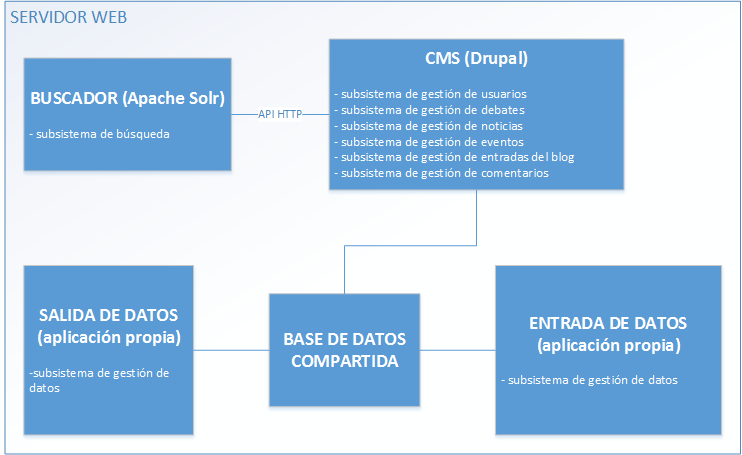
\includegraphics[width=\textwidth]{diagrama_subsistemas.png}
\caption{Diagrama de subsistemas}
\label{fig:diagrama_subsistemas}
\end{figure}


\section{Especificación de casos de uso}
\label{especificacion_casos_uso}
En esta sección se detallarán los casos de uso del sistema.  Para facilitar la lectura, los casos de uso y escenarios se agruparán por subsistemas.

Cada caso de uso tendrá la siguiente información:
\begin{itemize}
\item Nombre.  Nombre que permita identificar al caso de uso.
\item Precondiciones.  Las precondiciones indican una situación que es de obligado cumplimiento antes del caso de uso.  Por simplicidad, las precondiciones se omitirán en los casos de uso en los que no existan.
\item Descripción.  La descripción indica de forma resumida la finalidad del caso de uso.
\item Actores.  Los actores serán todos aquellos posibles participantes en el caso de uso.
\item Escenario principal.  El escenario principal indica de forma ordenada los pasos que se realizan en el caso de uso.
\item Escenarios alternativos.  Los escenarios alternativos representan variaciones o divergencias respecto al escenario principal.  Por simplicidad, los escenarios alternativos se omitirán en los casos de uso en los que no existan.
\end{itemize}


\subsection{Subsistema de gestión de usuarios}
\label{casos_uso_subsistema_usuarios}
En esta sección se detallarán los casos de uso y escenarios pertenecientes al subsistema de gestión de usuarios.
La figura \ref{fig:casos_uso_subsistema_usuarios} muestra el diagrama de casos de dicho subsistema.

\begin{figure}[h]
\centering
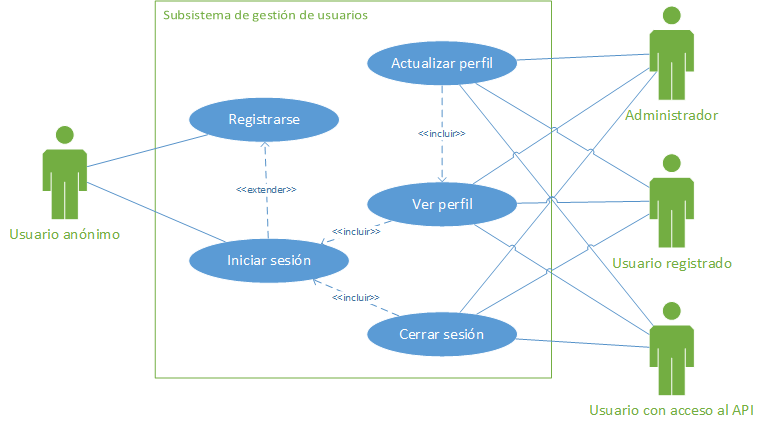
\includegraphics[width=\textwidth]{casos_uso_usuarios.png}
\caption{Diagrama de casos de uso del subsistema de gestión de usuarios}
\label{fig:casos_uso_subsistema_usuarios}
\end{figure}


\subsubsection{Caso de uso ``registrarse''}
\begin{description}
\item[Descripción] 				El usuario no dispone de una cuenta en el sistema y quiere crear una.
\item[Actores]					Cualquier usuario anónimo.
\item[Escenario principal]	 	\hfill
								\begin{enumerate}
								\item El usuario accede al formulario de registro.
								\item Una vez en el formulario de registro, el usuario rellena todos los campos requeridos.
								\item Si el usuario lo decide también puede rellenar los campos opcionales.
								\item Tras rellenar los campos el usuario pulsa el botón de registro.
								\item El sistema guarda los datos y crea la nueva cuenta de usuario con estado bloqueado.
								\end{enumerate}
\item[Escenario alternativo 1]	El usuario no rellena todos los campos necesarios.
								\begin{enumerate}
								\item Cuando el usuario pulse el botón para completar el registro el sistema notificará del error.
								\item Se continuará desde el punto 2 del escenario principal.
								\end{enumerate}
\item[Escenario alternativo 2]	El nombre de usuario ya existe en el sistema.
								\begin{enumerate}
								\item Cuando el usuario pulse el botón para completar el registro el sistema notificará del error.
								\item Se continuará desde el punto 2 del escenario principal.
								\end{enumerate}
\item[Escenario alternativo 3]	El email de usuario ya existe en el sistema.
								\begin{enumerate}
								\item Cuando el usuario pulse el botón para completar el registro el sistema notificará del error.
								\item Se continuará desde el punto 2 del escenario principal.
								\end{enumerate}
\end{description}


\subsubsection{Caso de uso ``activar usuario''}
\begin{description}
\item[Descripción] 				El administrador activa una cuenta de un usuario para que éste pueda utilizarla.
\item[Actores]					El administrador del sistema.
\item[Precondiciones]			La cuenta de usuario debe ser registrada previamente en el sistema.
\item[Escenario principal]	 	\hfill
								\begin{enumerate}
								\item El administrador accede al panel de administración.
								\item Una vez en el panel de administración, accede a la vista de usuarios.
								\item El administrador selecciona el usuario o usuarios a activar.
								\item Pulsa el botón correspondiente para activar los usuarios.
								\item El sistema actualiza el estado de los usuarios y permite que inicien sesión en el sistema.
								\end{enumerate}
\end{description}


\subsubsection{Caso de uso ``iniciar sesión''}
\begin{description}
\item[Descripción] El usuario accede al sistema utilizando su nombre de usuario y contraseña.
\item[Actores] Cualquier usuario anónimo.
\item[Precondiciones] La cuenta de usuario con la que se inicia sesión ha sido activada por un administrador.
\item[Escenario principal] \hfill
						 	\begin{enumerate}
							\item El usuario accede al formulario de inicio de sesión
							\item El usuario introduce su nombre de usuario
							\item El usuario introduce su contraseña
							\item El usuario inicia sesión pulsando el botón correspondiente
							\end{enumerate}
\item[Escenario alternativo 1] El usuario no existe
							\begin{enumerate}
							\item El sistema notificará al usuario de que el nombre de usuario introducido no existe
							\item Se continuará desde el paso 2 del escenario principal
							\end{enumerate}
\item [Escenario alternativo 2] La contraseña es incorrecta
							\begin{enumerate}
							\item El sistema notificará al usuario de que la contraseña introducida es incorrecta
							\item Se continuará desde el paso 2 del escenario principal
							\end{enumerate}							
\end{description}


\subsubsection{Caso de uso ``cerrar sesión''}
\begin{description}
\item[Descripción] 			El usuario quiere cerrar su sesión en el sistema.
\item[Actores] 				Administrador, usuario registrado o usuario con capacidad de acceso al API.
\item[Precondiciones]  		Haber iniciado sesión en el sistema
\item[Escenario principal] 	\hfill
						 	\begin{enumerate}
							\item El usuario con sesión iniciada pulsa en el botón para cerrar sesión.
							\item El sistema redirige al usuario a la vista principal con la sesión ya cerrada.
							\end{enumerate}							
\end{description}


\subsubsection{Caso de uso ``ver perfil''}
\begin{description}
\item[Descripción] 			El usuario quiere ver la información sobre su cuenta almacenada en el sistema.
\item[Actores] 				Administrador, usuario registrado o usuario con capacidad de acceso al API.
\item[Precondiciones]  		Haber iniciado sesión en el sistema
\item[Escenario principal] 	\hfill
						 	\begin{enumerate}
							\item El usuario con sesión iniciada pulsa en el botón para ver su información.
							\item El sistema muestra una vista de la cuenta del usuario con todos los datos almacenados.
							\end{enumerate}
\item[Escenario alternativo 1] El usuario cuenta con capacidad de acceso al API
							\begin{enumerate}
							\item Similar al escenario principal, pero el sistema mostrará también el \textit{token} de acceso al API.
							\end{enumerate}
\item [Escenario alternativo 2] Acceso a un perfil no propio.
							\begin{enumerate}
							\item El usuario pulsa en el perfil de otro usuario del sistema.
							\item El sistema muestra una vista de la cuenta de usuario.
							\item El sistema no muestra en ningún caso el \textit{token} de acceso al API.
							\end{enumerate}							
\end{description}


\subsubsection{Caso de uso ``actualizar perfil''}
\begin{description}
\item[Descripción] 			El usuario quiere modificar la información almacenada en el sistema sobre su cuenta.
\item[Actores] 				Administrador, usuario registrado o usuario con capacidad de acceso al API.
\item[Precondiciones]  		Haber iniciado sesión en el sistema
\item[Escenario principal] 	\hfill
						 	\begin{enumerate}
							\item El usuario con sesión iniciada pulsa en el botón para ver su información.
							\item Una vez en la vista del perfil, el usuario pulsa el botón para modificar su información.
							\item El usuario modifica los datos que considere necesarios.
							\item El usuario introduce su contraseña actual para asegurar su identidad.
							\item El sistema actualiza la información de la cuenta de usuario.
							\end{enumerate}
\item[Escenario alternativo 1] La contraseña actual no es válida.
							\begin{enumerate}
							\item El sistema informará al usuario de su error y no modificará la información almacenada.
							\item Se continua desde el punto 3 del escenario principal.
							\end{enumerate}
\item [Escenario alternativo 2] El usuario quiere modificar su contraseña.
							\begin{enumerate}
							\item El usuario debe introducir su nueva contraseña dos veces para evitar errores.
							\item Se continua desde el punto 4 del escenario principal.
							\end{enumerate}							
\item [Escenario alternativo 3] Las nuevas contraseñas no coinciden.
							\begin{enumerate}
							\item Las nuevas contraseñas introducidas no coinciden.
							\item El sistema informa al usuario del error.
							\item Se continua desde el punto 1 del escenario alternativo 2.
							\end{enumerate}							
\item[Escenario alternativo 4] El nuevo correo es inválido o ya existe en el sistema.
							\begin{enumerate}
							\item El sistema informará al usuario de su error y no modificará la información almacenada.
							\item Se continua desde el punto 3 del escenario principal.
							\end{enumerate}							
\end{description}

\subsection{Subsistema de gestión de debates}
\label{casos_uso_subsistema_debates}
En esta sección se detallarán los casos de uso y escenarios pertenecientes al subsistema de gestión de debates.
La figura \ref{fig:casos_uso_subsistema_debates} muestra el diagrama de casos de uso del subsistema de gestión de debates.

\begin{figure}[h]
\centering
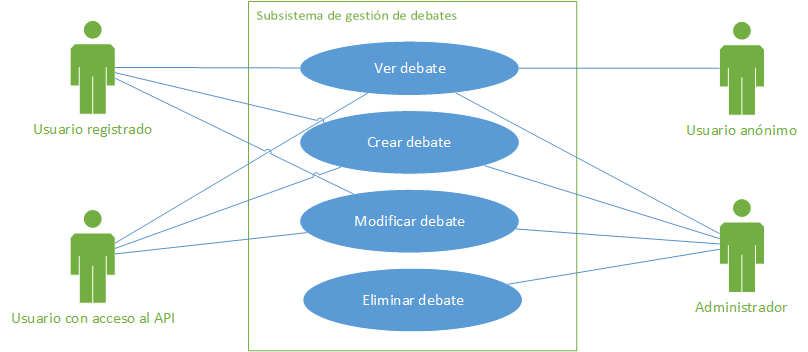
\includegraphics[width=\textwidth]{casos_uso_debates.png}
\caption{Diagrama de casos de uso del subsistema de gestión de debates}
\label{fig:casos_uso_subsistema_debates}
\end{figure}


\subsubsection{Caso de uso ``ver debate''}
\begin{description}
\item[Descripción] 				El usuario quiere ver el contenidos y los comentarios de un debate.
\item[Actores]					Cualquier usuario registrado o no en el sistema.
\item[Escenario principal]	 	\hfill
								\begin{enumerate}
								\item El usuario pulsa en el botón que carga la vista de los debates.
								\item Una vez en la vista de debates, elige el debate del que quiere ver sus contenidos.
								\item El usuario pulsa en el título del debate elegido.
								\item El sistema carga la vista del debate mostrando tanto el contenido como los comentarios del mismo.
								\end{enumerate}
\item[Escenario alternativo 1]	El usuario utiliza la búsqueda para localizar el debate.
								\begin{enumerate}
								\item El usuario accede a la vista de la búsqueda.
								\item El usuario escribe algunas palabras que se encuentren en el debate que quiere visualizar.
								\item En la lista de resultados selecciona el debate que desee.
								\item Se continua desde el punto 4 del escenario principal.
								\end{enumerate}
\end{description}


\subsubsection{Caso de uso ``crear debate''}
\begin{description}
\item[Descripción] El usuario quiere crear un nuevo debate para que puedan participar el resto de usuarios.
\item[Actores] Administrador, usuario registrado o usuario con capacidad de acceso al API.
\item[Precondiciones] Haber iniciado sesión en el sistema.
\item[Escenario principal] \hfill
						 	\begin{enumerate}
							\item El usuario accede a la vista de debates.
							\item Pulsa el botón para crear un debate.
							\item Rellena los campos requeridos en el formulario de creación del debate.
							\item Rellena los campos opcionales que considere necesarios en el formulario de creación del debate.
							\item Pulsa el botón para guardar el debate.
							\item El sistema guarda el debate con estado ``próximamente''.
							\end{enumerate}
\item[Escenario alternativo 1] El usuario no ha rellenado todos los campos requeridos.
							\begin{enumerate}
							\item El sistema notificará al usuario de que faltan campos por rellenar.
							\item Se continuará desde el punto 3 del escenario principal.
							\end{enumerate}
\end{description}


\subsubsection{Caso de uso ``comentar un debate''}
\begin{description}
\item[Descripción] El usuario quiere crear dar su opinión en un debate abierto.
\item[Actores] Administrador, usuario registrado o usuario con capacidad de acceso al API.
\item[Precondiciones] Haber iniciado sesión en el sistema.
\item[Escenario principal] \hfill
						 	\begin{enumerate}
							\item El usuario accede a la vista de debates.
							\item Selecciona el debate en el que quiere crear un comentario.
							\item Una vez en la vista del debate, el usuario escribe su comentario.
							\item Pulsa el botón de para guardar su comentario.
							\end{enumerate}
\item[Escenario alternativo 1] El usuario quiere añadir un comentario como respuesta a otro comentario ya existente.
							\begin{enumerate}
							\item Los dos primeros pasos serán similares a los del escenario principal.
							\item Una vez en la vista de debate el usuario localiza el comentario al que quiere responder y pulsa el botón correspondiente.
							\item El usuario escribe su comentario.
							\item Pulsa el botón para guardar el comentario.
							\end{enumerate}
\end{description}


\subsubsection{Caso de uso ``modificar comentario''}
\begin{description}
\item[Descripción] El usuario quiere crear modificar un comentario que ha creado previamente.
\item[Actores] Administrador, usuario registrado o usuario con capacidad de acceso al API.
\item[Precondiciones] Haber iniciado sesión en el sistema.
\item[Escenario principal] \hfill
						 	\begin{enumerate}
							\item El usuario accede a la vista de debates.
							\item Selecciona el debate en el que ha realizado el comentario que quiere modificar.
							\item Una vez en la vista del debate busca su comentario y pulsa el botón destinado a modificarlo.
							\item Introduce el nuevo texto del comentario
							\item Pulsa el botón de para guardar su comentario.
							\end{enumerate}
\end{description}


\subsubsection{Caso de uso ``moodificar debate''}
\begin{description}
\item[Descripción] Un usuario quiere modificar el contenido de un debate.
\item[Actores] Administrador, usuario registrado o usuario con capacidad de acceso al API.
\item[Precondiciones] Haber iniciado sesión en el sistema.
\item[Escenario principal] \hfill
						 	\begin{enumerate}
							\item El usuario accede a la vista de debates.
							\item Selecciona el debate cuyo contenido desea modificar.
							\item Una vez en la vista del debate pulsa el botón destinado a modificarlo.
							\item Modifica la información que sea necesaria (excepto el estado del debate, el proceso de modificación del estado de un debate está descrito en el escenario alternativo 1).
							\item Pulsa el botón de para guardar las modificaciones.
							\item El sistema actualiza los contenidos del debate.
							\end{enumerate}
\item[Escenario alternativo 1]  Modificar el estado de un debate.
							\begin{enumerate}
							\item El administrador accede al panel de administración.
							\item Selecciona el debate que desea modificar y pulsa el botón correspondiente.
							\item En la vista de edición del debate selecciona el nuevo estado que desea asignarle.
							\item Se continúa desde el punto 5 del escenario principal.
							\end{enumerate}
\item[Escenario alternativo 2]  No se rellenan todos los campos requeridos
							\begin{enumerate}
							\item El sistema informa al usuario del error y no modifica la información almacenada.
							\item Se continúa desde el punto 4 del escenario principal.
							\end{enumerate}
\end{description}


\subsubsection{Caso de uso ``eliminar debate''}
\begin{description}
\item[Descripción] El administrador quiere eliminar un debate junto con todos sus comentarios.
\item[Actores] Administrador.
\item[Precondiciones] Haber iniciado sesión en el sistema.
\item[Escenario principal] \hfill
						 	\begin{enumerate}
							\item El administardor accede a la vista de administración.
							\item Localiza el debate que desea eliminar y pulsa el botón correspondiente.
							\item El debate y sus comentarios serán eliminados del sistema.
							\end{enumerate}
\end{description}

\subsection{Subsistema de gestión de eventos}
\label{casos_uso_subsistema_eventos}
En esta sección se detallarán los casos de uso pertenecientes al subsistema de gestión de eventos. La figura \ref{fig:casos_uso_subsistema_eventos} muestra el diagrama de casos de uso de dicho subsistema.

\begin{figure}[h]
\centering
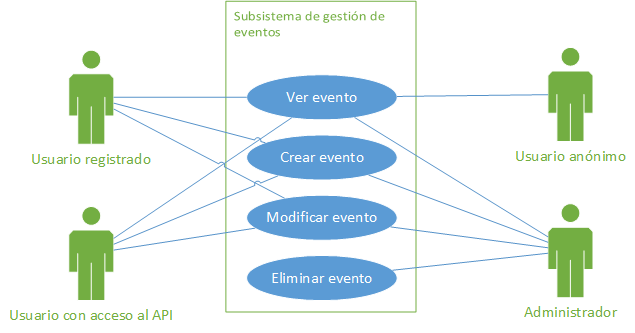
\includegraphics[width=\textwidth]{casos_uso_eventos}
\caption{Diagrama de casos de uso del subsistema de gestión de eventos}
\label{fig:casos_uso_subsistema_eventos}
\end{figure}


\subsubsection{Caso de uso ``ver evento''}
\begin{description}
\item[Descripción] Un usuario quiere ver el contenido de un evento.
\item[Actores] Cualquier usuario registrado o no en el sistema.
\item[Escenario principal] 	\hfill
							\begin{enumerate}
							\item El usuario accede a la vista de eventos.
							\item Una vez en la vista de eventos, elige el evento del que quiere ver sus contenidos.
							\item Pulsa en el título del evento que quiere ver en detalle.
							\item El sistema carga la vista del evento mostrando todos sus detalles.
							\end{enumerate}
\end{description}


\subsubsection{Caso de uso ``crear evento''}
\begin{description}
\item[Descripción]  Un usuario quiere añadir un nuevo evento al sistema.
\item[Actores]  Administrador, usuario registrado o usuario con capacidad de acceso al API.
\item[Precondiciones] Haber iniciado sesión en el sistema.
\item[Escenario principal]  \hfill
							\begin{enumerate}
							\item El usuario accede a la vista de los eventos.
							\item Una vez en la vista de eventos pulsa el botón correspondiente para crear un evento nuevo.
							\item Rellena el formulario con los datos requeridos.
							\item Si lo desea también rellena la información opcional del formulario.
							\item El usuario pulsa el botón guardar, y el sistema crea el nuevo evento.
							\end{enumerate}
\item[Escenario alternativo 1] No se han rellenado todos los campos requeridos.
							\begin{enumerate}
							\item El usuario no ha rellenado todos los campos requeridos para crear un nuevo evento.
							\item El sistema notificará al usuario de su error y no creará el nuevo evento.
							\item Se continuará desde el punto 3 del escenario principal.
							\end{enumerate}
\end{description}


\subsubsection{Caso de uso ``modificar evento''}
\begin{description}
\item[Descripción]  Un usuario quiere modificar un evento del sistema.
\item[Actores]  Administrador, usuario registrado o usuario con capacidad de acceso al API.
\item[Precondiciones]  Haber iniciado sesión en el sistema.
\item[Escenario principal]	\hfill
							\begin{enumerate}
							\item El usuario accede a la vista de los eventos..
							\item Una vez en la vista de eventos localiza el evento que quiere modificar.
							\item Cuando ha accedido al evento pulsa el botón correspondiente para modificar su contenido.
							\item Rellena toda la información requerida en el formulario.
							\item Si lo desea también rellena la información opcional del formulario.
							\item El usuario pulas el botón guardar y el sistema modifica la información del evento.
							\end{enumerate}
\item[Escenario alternativo 1] No se han rellenado todos los campos requeridos.
							\begin{enumerate}
							\item El usuario no ha rellenado todos los campos requeridos para modificar el evento.
							\item El sistema notificará al usuario de su error y no modificará los datos del evento.
							\item Se continuará desde el punto 4 del escenario principal.
							\end{enumerate}
\end{description}


\subsubsection{Caso de uso ``eliminar evento''}
\begin{description}
\item[Descripción]  Un administrador quiere eliminar un evento del sistema.
\item[Actores] El administrador del sistema.
\item[Precondiciones]  Haber iniciado sesión en el sistema.
\item[Escenario principal]	\hfill
							\begin{enumerate}
							\item El administrador accede a la vista de administración.
							\item Localiza el evento que desea eliminar y pulsa el botón correspondiente.
							\item El evento será eliminado del sistema.
							\end{enumerate}
\end{description}

\subsection{Subsistema de gestión de noticias}
\label{casos_uso_subsistema_noticias}
En esta sección se detallarán los casos de uso pertenecientes al subsistema de gestión de noticias. La figura \ref{fig:casos_uso_subsistema_noticias} muestra el diagrama de casos de uso de dicho subsistema.

\begin{figure}[h]
\centering
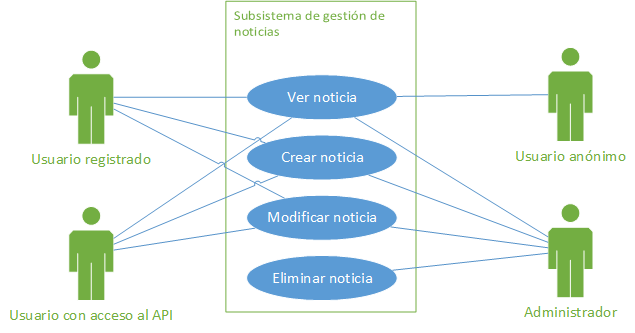
\includegraphics[width=\textwidth]{casos_uso_noticias}
\caption{Diagrama de casos de uso del subsistema de gestión de noticias}
\label{fig:casos_uso_subsistema_noticias}
\end{figure}


\subsubsection{Caso de uso ``ver noticia''}
\begin{description}
\item[Descripción] Un usuario quiere ver el contenido de una noticia.
\item[Actores] Cualquier usuario registrado o no en el sistema.
\item[Escenario principal] 	\hfill
							\begin{enumerate}
							\item El usuario pulsa en el botón que carga la vista de las noticias.
							\item Una vez en la vista de noticias pulsa en el título de la noticia que quiere ver en detalle.
							\item El sistema carga la vista de la noticia mostrando todos sus detalles.
							\end{enumerate}
\end{description}


\subsubsection{Caso de uso ``crear noticia''}
\begin{description}
\item[Descripción]  Un usuario quiere añadir una nueva noticia al sistema.
\item[Actores]  Administrador, usuario registrado o usuario con capacidad de acceso al API.
\item[Precondiciones] Haber iniciado sesión en el sistema.
\item[Escenario principal]  \hfill
							\begin{enumerate}
							\item El usuario pulsa en el botón que carga la vista de las noticias.
							\item Una vez en la vista de las noticias pulsa el botón correspondiente para crear una noticia nueva.
							\item Rellena el formulario con los datos requeridos.
							\item Si lo desea también rellena la información opcional del formulario.
							\item El usuario pulsa el botón guardar.
							\item El sistema crea la nueva noticia.
							\end{enumerate}
\item[Escenario alternativo 1] No se han rellenado todos los campos requeridos.
							\begin{enumerate}
							\item El usuario no ha rellenado todos los campos requeridos para crear una nueva noticia.
							\item El sistema notificará al usuario de su error y no creará la nueva noticia.
							\item Se continuará desde el punto 3 del escenario principal.
							\end{enumerate}
\end{description}


\subsubsection{Caso de uso ``modificar noticia''}
\begin{description}
\item[Descripción]  Un usuario quiere modificar una noticia del sistema.
\item[Actores]  Administrador, usuario registrado o usuario con capacidad de acceso al API.
\item[Precondiciones]  Haber iniciado sesión en el sistema.
\item[Escenario principal]	\hfill
							\begin{enumerate}
							\item El usuario accede a la vista de las noticias.
							\item Una vez en la vista de noticias localiza la noticia que quiere modificar.
							\item Cuando ha accedido a la noticia pulsa el botón correspondiente para modificar su contenido.
							\item Rellena toda la información requerida en el formulario.
							\item Si lo desea también rellena la información opcional del formulario.
							\item El usuario pulas el botón guardar.
							\item El sistema actualiza la información de la noticia editada.
							\end{enumerate}
\item[Escenario alternativo 1] No se han rellenado todos los campos requeridos.
							\begin{enumerate}
							\item El usuario no ha rellenado todos los campos requeridos para modificar la noticia.
							\item El sistema notificará al usuario de su error y no modificará los datos la noticia.
							\item Se continuará desde el punto 4 del escenario principal.
							\end{enumerate}
\end{description}


\subsubsection{Caso de uso ``eliminar noticia''}
\begin{description}
\item[Descripción]  Un administrador quiere eliminar una noticia del sistema.
\item[Actores]  El administrador del sistema.
\item[Precondiciones]  Haber iniciado sesión en el sistema.
\item[Escenario principal]	\hfill
							\begin{enumerate}
							\item El administrador accede a la vista de administración.
							\item Localiza la noticia que desea eliminar y pulsa el botón correspondiente.
							\item La noticia será eliminado del sistema.
							\end{enumerate}
\end{description}

\subsection{Subsistema de gestión del blog}
\label{casos_uso_subsistema_blog}
En esta sección se detallarán los casos de uso y escenarios pertenecientes al subsistema de gestión de entradas del blog. La figura \ref{fig:casos_uso_subsistema_blog} muestra el diagrama de casos de uso del subsistema de gestión de debates.

\begin{figure}[h]
\centering
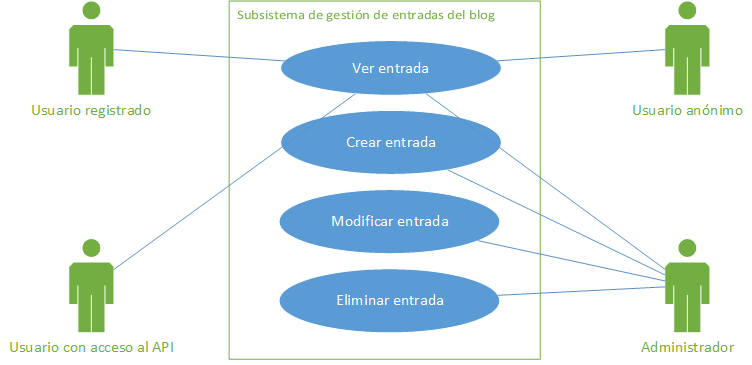
\includegraphics[width=\textwidth]{casos_uso_blog}
\caption{Diagrama de casos de uso del subsistema de gestión de entradas del blog}
\label{fig:casos_uso_subsistema_blog}
\end{figure}


\subsubsection{Caso de uso ``ver entrada''}
\begin{description}
\item[Descripción] 				El usuario quiere ver el contenido de una entrada del blog.
\item[Actores]					Cualquier rol de usuario.
\item[Escenario principal]	 	\hfill
								\begin{enumerate}
								\item El usuario accede al blog del Land Portal.
								\item Una vez en el blog, selecciona la entrada que quiere ver en detalle.
								\item El sistema carga la vista de la entrada mostrando tanto su contenido como sus comentarios.
								\end{enumerate}
\end{description}


\subsubsection{Caso de uso ``crear entrada''}
\begin{description}
\item[Descripción] El administrador quiere crear una nueva entrada en el blog del Land Portal.
\item[Actores] Administrador.
\item[Precondiciones] Haber iniciado sesión en el sistema.
\item[Escenario principal] \hfill
						 	\begin{enumerate}
							\item El administrador accede al blog del Land Portal.
							\item Una vez en el blog, el administrador pulsa el botón para crear una nueva entrada.
							\item Rellena los campos requeridos en el formulario de creación de la entrada.
							\item Rellena los campos opcionales que considere necesarios en el formulario de creación de la entrada.
							\item Pulsa el botón para guardar la entrada.
							\item El sistema guarda la entrada y la hace visible para todos los usuarios en el blog.
							\end{enumerate}
\item[Escenario alternativo 1] El administrador no ha rellenado todos los campos requeridos.
							\begin{enumerate}
							\item El sistema notificará al usuario de que faltan campos por rellenar.
							\item Se continuará desde el punto 3 del escenario principal.
							\end{enumerate}
\end{description}


\subsubsection{Caso de uso ``modificar entrada''}
\begin{description}
\item[Descripción] El administrador quiere modificar el contenido de una entrada del blog.
\item[Actores] El administrador del sistema.
\item[Precondiciones] Haber iniciado sesión en el sistema.
\item[Escenario principal] \hfill
						 	\begin{enumerate}
							\item El administrador accede al blog del Land Portal.
							\item Una vez en el blog, el administrador selecciona la entrada que quiere modificar.
							\item En la entrada correspondiente, el administrador pulsa el botón para editar su contenido.
							\item Rellena los campos requeridos en el formulario de modificación de la entrada.
							\item Rellena los campos opcionales que considere necesarios en el formulario de modificación de la entrada.
							\item Pulsa el botón para guardar los cambios
							\item El sistema actualiza los contenidos de la entrada del blog.
							\end{enumerate}
\item[Escenario alternativo 1]  No se rellenan todos los campos requeridos
							\begin{enumerate}
							\item El sistema informa al usuario del error y no modifica la información almacenada.
							\item Se continúa desde el punto 4 del escenario principal.
							\end{enumerate}
\end{description}

\subsubsection{Caso de uso ``eliminar entrada''}
\begin{description}
\item[Descripción] El administrador quiere eliminar una entrada del blog junto con todos sus comentarios.
\item[Actores] El administrador del sistema.
\item[Precondiciones] Haber iniciado sesión en el sistema.
\item[Escenario principal] \hfill
						 	\begin{enumerate}
							\item El administrador accede a la vista de administración.
							\item En la sección de contenidos localiza la entrada y pulsa el botón correspondiente para eliminarla.
							\item La entrada y sus comentarios serán eliminados del sistema.
							\end{enumerate}
\end{description}



\subsection{Subsistema de gestión de comentarios}
\label{casos_uso_subsistema_comentarios}
En esta sección se detallarán los casos de uso y escenarios pertenecientes al subsistema de gestión de comentarios. La figura \ref{fig:casos_uso_subsistema_comentarios} muestra el diagrama de casos de uso de dicho subsistema.

\begin{figure}[h]
\centering
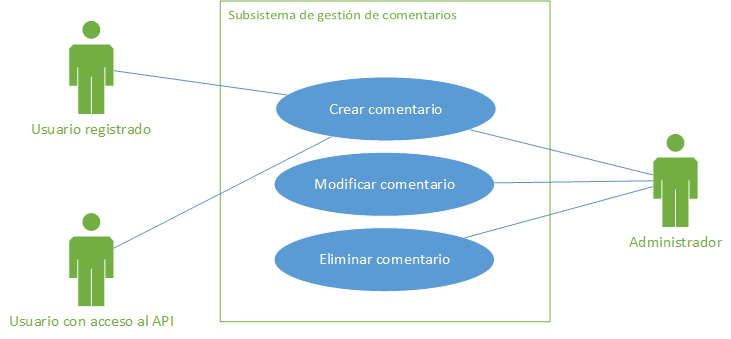
\includegraphics[width=\textwidth]{casos_uso_comentarios}
\caption{Diagrama de casos de uso del subsistema de gestión de comentarios}
\label{fig:casos_uso_subsistema_comentarios}
\end{figure}


\subsubsection{Caso de uso ``crear comentario''}
\begin{description}
\item[Descripción] El usuario quiere crear un nuevo comentario.
\item[Actores] Administrador, usuario registrado o usuario con capacidad de acceso al API.
\item[Precondiciones] Haber iniciado sesión en el sistema.
\item[Escenario principal] \hfill
						 	\begin{enumerate}
							\item El usuario accede a la entrada del blog o al debate en el que quiere crear el comentario.
							\item El usuario escribe su comentario.
							\item Pulsa el botón de para guardar su comentario.
							\item El sistema guarda el comentario y lo hace visible al resto de usuarios.
							\end{enumerate}
\item[Escenario alternativo 1] Comentario en un  debate cerrado.
							\begin{enumerate}
							\item El usuario accede al debate en el que quiere crear el comentario.
							\item El sistema no mostrará opciones para que el usuario cree un comentario.
							\end{enumerate}
\end{description}


\subsubsection{Caso de uso ``modificar comentario''}
\begin{description}
\item[Descripción] El administrador desea modificar el contenido de un comentario realizado por un usuario.
\item[Actores] Administrador.
\item[Precondiciones] Haber iniciado sesión en el sistema.
\item[Escenario principal] \hfill
						 	\begin{enumerate}
							\item El usuario accede a la entrada del blog o al debate en el que se encuentra el comentario a modificar.
							\item El administrador localiza el comentario y pulsa el botón modificar.
							\item El administrador introduce el texto que crea conveniente y pulsa el botón guardar.
							\item El sistema actualiza el contenido del comentario modificado.
							\end{enumerate}
\end{description}


\subsubsection{Caso de uso ``eliminar comentario''}
\begin{description}
\item[Descripción] El administrador desea eliminar un comentario realizado por un usuario.
\item[Actores] Administrador.
\item[Precondiciones] Haber iniciado sesión en el sistema.
\item[Escenario principal] \hfill
						 	\begin{enumerate}
							\item El usuario accede a la entrada del blog o al debate en el que se encuentra el comentario a eliminar.
							\item El administrador localiza el comentario y pulsa el botón eliminar.
							\item El sistema elimina el comentario y deja de mostrarlo.
							\end{enumerate}
\end{description}

\subsection{Subsistema de gestión de organizaciones}
\label{casos_uso_subsistema_organizaciones}
En esta sección se detallarán los casos de uso pertenecientes al subsistema de gestión de organizaciones. La figura \ref{fig:casos_uso_subsistema_organizaciones} muestra el diagrama de casos de uso de dicho subsistema.

\begin{figure}[h]
\centering
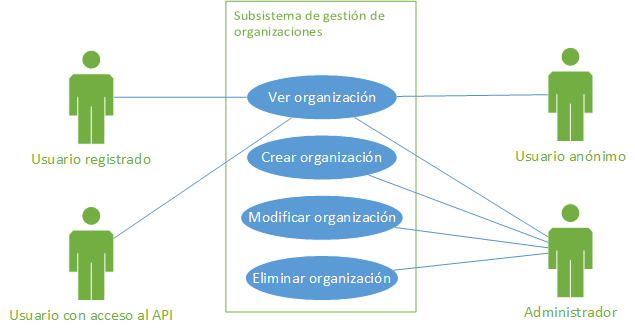
\includegraphics[width=\textwidth]{casos_uso_organizaciones}
\caption{Diagrama de casos de uso del subsistema de gestión de organizaciones}
\label{fig:casos_uso_subsistema_organizaciones}
\end{figure}


\subsubsection{Caso de uso ``ver organización''}
\begin{description}
\item[Descripción] Un usuario quiere ver la información sobre una organización.
\item[Actores] Cualquier usuario registrado o no en el sistema.
\item[Escenario principal] 	\hfill
							\begin{enumerate}
							\item El usuario pulsa en el botón que carga la vista de las organizaciones.
							\item Una vez en la vista de organizaciones pulsa en el nombre o la imagen de la organización que quiere ver en detalle.
							\item El sistema carga la vista de la organización mostrando todos sus detalles.
							\end{enumerate}
\end{description}


\subsubsection{Caso de uso ``crear organización''}
\begin{description}
\item[Descripción]  Un administrador quiere añadir una nueva organización al sistema.
\item[Actores]  El administrador del sistema.
\item[Precondiciones] Haber iniciado sesión en el sistema.
\item[Escenario principal]  \hfill
							\begin{enumerate}
							\item El usuario pulsa en el botón que carga la vista de las organizaciones.
							\item Una vez en la vista de las organizaciones pulsa el botón correspondiente para crear una organización nueva.
							\item Rellena el formulario con los datos requeridos.
							\item Si lo desea también rellena la información opcional del formulario.
							\item El administrador pulsa el botón guardar.
							\item El sistema crea la nueva noticia.
							\end{enumerate}
\item[Escenario alternativo 1] No se han rellenado todos los campos requeridos.
							\begin{enumerate}
							\item El administrador no ha rellenado todos los campos requeridos para crear una nueva organización.
							\item El sistema notificará al administrador de su error y no creará la nueva organización.
							\item Se continuará desde el punto 3 del escenario principal.
							\end{enumerate}
\end{description}


\subsubsection{Caso de uso ``modificar organización''}
\begin{description}
\item[Descripción]  Un administrador quiere modificar una organización existente en el sistema.
\item[Actores]  El administrador del sistema.
\item[Precondiciones] Haber iniciado sesión en el sistema.
\item[Escenario principal]	\hfill
							\begin{enumerate}
							\item El usuario accede a la vista de las organizaciones.
							\item Una vez en la vista de noticias localiza la organización que quiere modificar.
							\item Cuando ha accedido a la organización pulsa el botón correspondiente para modificar su contenido.
							\item Rellena toda la información requerida en el formulario.
							\item Si lo desea también rellena la información opcional del formulario.
							\item El administrador pulsa el botón guardar.
							\item El sistema actualiza la información de la organización editada.
							\end{enumerate}
\item[Escenario alternativo 1] No se han rellenado todos los campos requeridos.
							\begin{enumerate}
							\item El administrador no ha rellenado todos los campos requeridos para modificar la organización.
							\item El sistema notificará al usuario de su error y no modificará los datos de la organización.
							\item Se continuará desde el punto 4 del escenario principal.
							\end{enumerate}
\end{description}


\subsubsection{Caso de uso ``eliminar organización''}
\begin{description}
\item[Descripción]  Un administrador quiere eliminar una organización del sistema.
\item[Actores]  El administrador del sistema.
\item[Precondiciones]  Haber iniciado sesión en el sistema.
\item[Escenario principal]	\hfill
							\begin{enumerate}
							\item El administrador accede a la vista de las organizaciones.
							\item Accede a la organización que desea eliminar.
							\item Una vez en la vista de la organización pulsa el botón correspondiente para su eliminación.
							\item La organización será eliminada del sistema.
							\end{enumerate}
\end{description}

\subsection{Subsistema de búsqueda}
\label{casos_uso_subsistema_busqueda}
En esta sección se detallarán los casos de uso y escenarios pertenecientes al subsistema de búsqueda. La figura \ref{fig:casos_uso_subsistema_busqueda} muestra el diagrama de casos de uso de dicho subsistema.

\begin{figure}[h]
\centering
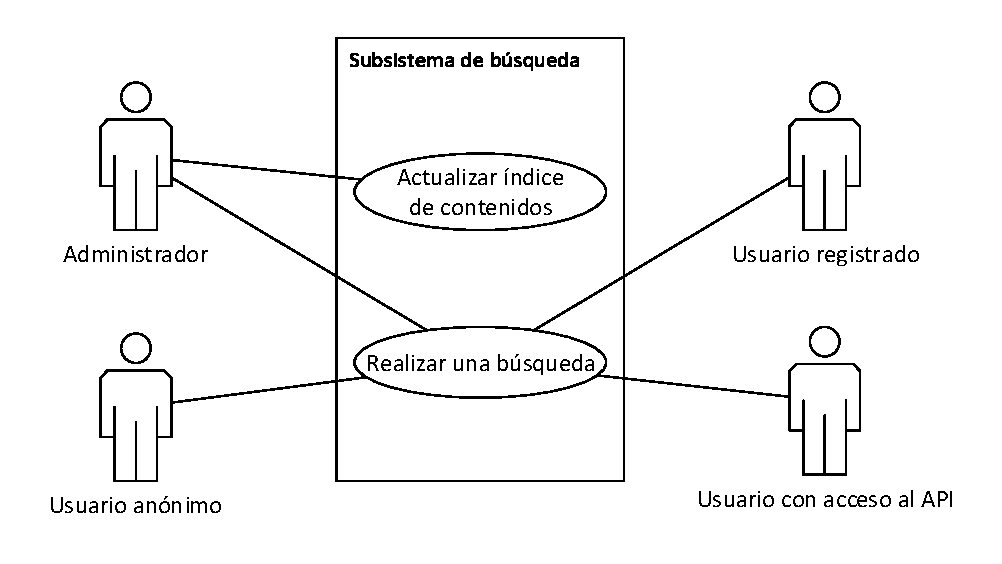
\includegraphics[width=\textwidth]{casos_uso/diagrama_casos_uso_busqueda}
\caption{Diagrama de casos de uso del subsistema de búsqueda}
\label{fig:casos_uso_subsistema_busqueda}
\end{figure}

\subsubsection{Caso de uso ``realizar una búsqueda''}
\begin{description}
\item[Descripción] Un usuario busca información en el sistema.
\item[Actores] Cualquier rol de usuario registrado o no en el sistema.
\item[Escenario principal] \hfill
							\begin{enumerate}
							\item El usuario introduce un texto en el formulario de búsqueda
							\item El usuario pulsa el botón de buscar
							\item El sistema devuelve los resultados correspondientes
							\end{enumerate}						
\end{description}

\subsubsection{Caso de uso ``actualizar índice de contenidos''}
\begin{description}
\item[Descripción] El administrador actualiza el índice de contenidos del subsistema de búsqueda.
\item[Actores] El administrador del sistema.
\item[Escenario principal] \hfill
							\begin{enumerate}
							\item El administrador accede al panel de administración.
							\item Una vez en el panel de administración, accede a las opciones de la búsqueda
							\item El administrador pulsa el botón correspondiente para realizar la regeneración del índice de contenidos.
							\item El sistema actualiza el índice de contenidos incluyendo los nuevos contenidos y eliminado los contenidos que ya no existan.
							\end{enumerate}						
\end{description}

\subsection{Subsistema de gestión de datos}
\label{casos_uso_subsistema_datos}
En esta sección se detallarán los casos de uso pertenecientes al subsistema de datos. La figura \ref{fig:casos_uso_subsistema_datos} muestra el diagrama de casos de uso de dicho subsistema.

\begin{figure}[h]
\centering
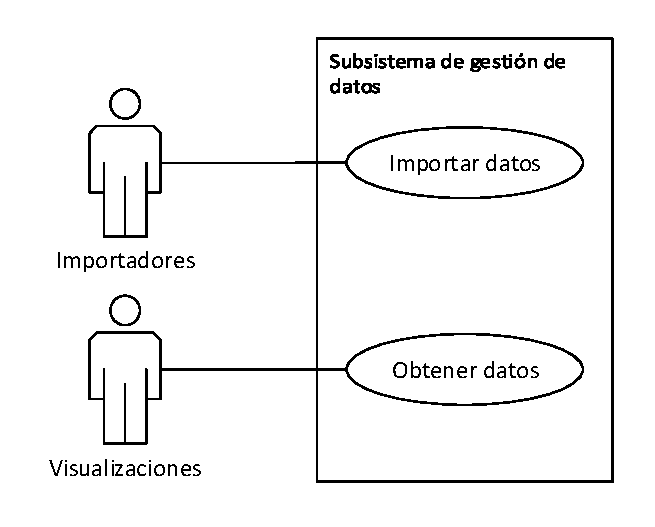
\includegraphics{casos_uso/diagrama_casos_uso_datos}
\caption{Diagrama de casos de uso del subsistema de datos}
\label{fig:casos_uso_subsistema_datos}
\end{figure}

\subsubsection{Caso de uso ``importar datos''}
\begin{description}
\item[Descripción] Un importador quiere incluir nueva información en el sistema.
\item[Actores] Un importador.
\item[Escenario principal] \hfill
							\begin{enumerate}
							\item El importador envía una petición POST al subsistema de datos incluyendo un fichero XML conforme a un XML Schema definido y con los datos a incluir en el sistema.
							\item El subsistema de datos comprueba si la dirección de origen de la petición está en la lista blanca.
							\item El subsistema de datos procesa la petición convirtiendo la información del fichero XML a un modelo propio.
							\item El subsistema de datos persiste en la base de datos el modelo creado anteriormente.
							\item El subsistema envía una respuesta 200 (\textit{OK}) al importador.
							\end{enumerate}
\item[Escenario alternativo 1] Los datos enviados por el importador no se ajustan al XML Schema.
							\begin{enumerate}
							\item El subsistema de datos no insertará ningún dato en la base de datos.
							\item El subsistema de datos envía una respuesta de error al importador.
							\end{enumerate}
\item[Escenario alternativo 2] El verbo utilizado por el importador no es el correcto (GET, PUT, etc).
							\begin{enumerate}
							\item El subsistema de datos no insertará ningún dato en la base de datos.
							\item El subsistema de datos envía una respuesta de error 405 (\textit{Method not Allowed}) al importador.
							\end{enumerate}
\item[Escenario alternativo 3] La petición realizada por el importador no incluye el fichero XML con los datos.
							\begin{enumerate}
							\item El subsistema de datos no insertará ningún dato en la base de datos.
							\item El subsistema de datos envía una respuesta de error 400 (\textit{Bad Request}) al importador.
							\end{enumerate}
\item[Escenario alternativo 4] La petición proviene de un origen no confiable
							\begin{enumerate}
							\item El subsistema de datos aborta la petición con un código de error 403 (\textit{Forbidden}).
							\end{enumerate}
\end{description}	

\subsubsection{Caso de uso ``obtener datos''}
\begin{description}
\item[Descripción] Una visualización pide datos para presentarlos al usuario de forma atractiva.
\item[Actores] Visualizaciones.
\item[Escenario principal] 	\hfill
							\begin{enumerate}
							\item La visualización lanza una petición GET al subsistema de datos.
							\item El subsistema de datos devuelve un fichero JSON con los datos correspondientes a la petición realizada.
							\item La visualización procesa los datos recibidos para presentarlos de forma visual.
							\end{enumerate}
\item[Escenario alternativo 1] La petición de la visualización es errónea.
							\begin{enumerate}
							\item La visualización lanza una petición al subsistema de datos.
							\item El subsistema de datos responde con un código de error HTTP.
							\end{enumerate}
\end{description}


\section{Clases preliminares del modelo}
\label{clases_preliminares_modelo}
En esta sección se realizará un análisis preliminar de las clases del sistema.  El objetivo de este análisis será mostrar una primera versión de los datos del modelo del sistema y de sus relaciones.

Para facilitar la lectura, se dividirá el análisis de clases en dos partes: una parte contendrá las clases pertenecientes a la zona social y la otra parte contendrá las clases pertenecientes a la zona de datos.


\subsection{Análisis preliminar de clases de la zona de datos}
\label{clases_preliminares_modelo_datos}
A continuación se realizará el análisis de las clases pertenecientes a la zona de datos. Como se ha explicado anteriormente en la sección \nameref{identificacion_subsistemas} perteneciente al capítulo \ref{chapter04}, la zona de datos incluye únicamente el subsistema de datos, que será el encargado de introducir datos en el sistema y devolverlos cuando sean pedidos por las visualizaciones.

La figura \ref{fig:clases_preliminares_modelo_book} muestra el diagrama de las clases preliminares de la zona datos.

\begin{landscape}
	\begin{figure}[ht]
		\centering
		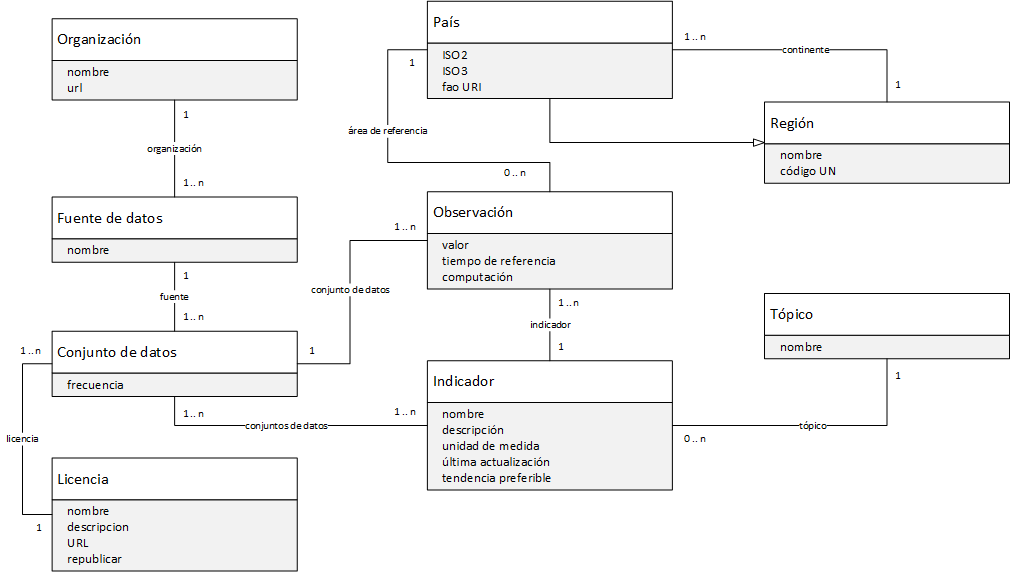
\includegraphics[height=\textwidth]{clases/clases_book_preliminar}
		\caption{Diagrama de clases preliminares de la zona de datos}
		\label{fig:clases_preliminares_modelo_book}
	\end{figure}
\end{landscape}


\subsubsection{Descripción de las clases}
\begin{description}
\item[Región]	Representa un país o continente del mundo.  Sus atributos son los siguientes:
							\begin{itemize}
								\item \textbf{Nombre}  Será el nombre de la región, por ejemplo ``Europa'', ``África'' o ``España''.
								\item \textbf{Código UN}  Será el código numérico asignado por la División Estadística de las Naciones Unidas\footnote{Éste código recibe el nombre formal de ``ISO 3166-1 numeric''.  En \cite{un:standard-country-codes} y \cite{un:iso-3166-country-codes} puede encontrarse más información sobre éstos códigos.} para la región.
							\end{itemize}
\item[País]  Representa a un país del mundo sobre el que se almacenarán observaciones.  Además de los atributos de una región, sus atributos serán:
							\begin{itemize}
							\item \textbf{ISO2}  Será el código alfabético de dos letras asignado por la división estadística de las Naciones Unidas\footnote{Éste código recibe el nombre formal de ``ISO 3166-1 alpha-2''. Se utiliza para hacer representar países, territorios independientes o zonas geográficas de interés especial. En \cite{un:iso-3166-country-codes} puede encontrarse más información sobre éstos códigos} para el país.
							\item \textbf{ISO3}  Será el código alfabético de tres letras asignado por la división estadística de las Naciones Unidas\footnote{Éste código recibe el nombre formal de ``ISO 3166-1 alpha-3''. Se utiliza para hacer representar países, territorios independientes o zonas geográficas de interés especial. En \cite{un:iso-3166-country-codes} puede encontrarse más información sobre éstos códigos} para el país.  El código ISO3 consigue una mejor asociación con los nombres de los países que el código ISO2.
							\item \textbf{FAO URI}  Será la URI única del país en la Ontología Geopolítica de la Organización para la Alimentación y la Agricultura de las Naciones Unidas\footnote{La información sobre ésta ontología se encuentra disponible en \cite{fao:geopolitical-ontology}}.
							\item \textbf{Continente}  Representa el continente del que el país forma parte.  Cada país forma parte de un continente, pero un continente puede estar compuesto de muchos países.
							\end{itemize}
\item[Observación]  Representa una medición realizada en un tiempo concreto para un país determinado.  Las observaciones son utilizadas por las visualizaciones para presentar los datos de forma visual a los usuarios.  Sus atributos serán los siguientes:
							\begin{itemize}
							\item \textbf{Valor}  Será el valor concreto de la observación.
							\item \textbf{Tiempo de referencia}  Será el tiempo al que hace referencia la observación.  Por ejemplo, el tiempo de referencia puede ser un año, un mes, un intervalo de años, etc.
							\item \textbf{Computación}  Indica el tipo de computación de la que proviene la observación.  Por ejemplo indica si el valor de la observación es único o un agregado de los valores durante un determinado periodo de tiempo.
							\item \textbf{Área de referencia}  Representa el país al que la observación hace referencia.  Cada observación hace referencia a un país, pero un país puede tener muchas observaciones que le hagan referencia.
							\item \textbf{Indicador}  Representa el indicador al que pertenece la observación.  Cada observación pertenece a un indicador, pero un indicador puede contener multitud de observaciones.
							\item \textbf{Conjunto de datos}  Representa el conjunto de datos del que proviene la observación.  Cada observación proviene de un único conjunto de datos, pero cada conjunto de datos incluye múltiples observaciones.
							\end{itemize}
\item[Indicador]  Representa un elemento sobre el que se realizan observaciones.  Sus atributos son lo siguientes:
							\begin{itemize}
							\item \textbf{Nombre}  Es un nombre corto para un indicador.
							\item \textbf{Descripción}  Es una descripción sobre lo que representa el indicador.  Por ejemplo ``Índice de Desarrollo Humano''\footnote{El Índice de Desarrollo Humano (HDI) es un indicador real mantenido por el United Nations Development Programme (UNDP) y que se encontrará en la zona de datos del portal final}.
							\item \textbf{Unidad de medida}  Representa la unidad de medida de las observaciones del indicador.  Por ejemplo el indicador ``propiedad de las tierras por parte de mujeres'' podría tener una unidad de medida en porcentaje.
							\item \textbf{Última actualización}  Indica la fecha de la última actualización del indicador o alguna de sus observaciones en el sistema.
							\item \textbf{Tendencia preferible}  Representa si es preferible que el valor del indicador crezca o disminuya a lo largo del tiempo.  Por ejemplo para el indicador ``mortalidad infantil'' la tendencia preferible será que disminuya.
							\item \textbf{Tópico}  Representa el tópico (categoría) en la que se incluye el indicador.  Cada indicador pertenece a un tópico, pero un tópico puede tener muchos indicadores relacionados.
							\item \textbf{Conjuntos de datos}  Representa los conjuntos de datos en los que el indicador está presente.  Un indicador puede estar presente en muchos conjuntos de datos y, al mismo tiempo, un conjunto de datos puede contener muchos indicadores diferentes.
							\end{itemize}
\item[Tópico]  Representa un categoría de indicadores que tratan sobre un mismo tema.  Sus atributos son lo siguientes:
							\begin{itemize}
							\item \textbf{Nombre}  Es el nombre del tópico.  Por ejemplo ``Tierra y género'' o ``Propiedad de la tierra''.
							\end{itemize}
\item[Conjunto de datos]  Representa un conjunto de datos que se inserta en el sistema.  Sus atributos son los siguientes:
							\begin{itemize}
							\item \textbf{Frecuencia}  Indica la frecuencia con la que se actualiza el conjunto de datos.  Algunas frecuencias de ejemplo pueden ser: ``anual'', ``trimestral'', etc.
							\item \textbf{Fuente}  Representa la fuente de la que proviene el conjunto de datos.  Cada conjunto de datos pertenece a una fuente, pero cada fuente puede contener varios conjuntos de datos.
							\item \textbf{Licencia}  Representa la licencia bajo la que se publica el conjunto de datos.  Cada conjunto de datos se publica bajo una licencia, pero cada licencia puede tener varios conjuntos de datos.
							\end{itemize}
\item[Licencia]  Representa una licencia bajo la que se publica un conjunto de datos.  Sus atributos son los siguientes:
							\begin{itemize}
							\item \textbf{Nombre}  Es el nombre corto de la licencia,  Por ejemplo  ``CC BY 2.0''.
							\item \textbf{Descripción}  Es una descripción larga sobre el funcionamiento de la licencia.
							\item \textbf{URL}  Será la URL bajo la que se encuentra disponible la información de la licencia  Por ejemplo \url{https://creativecommons.org/licenses/by/2.0/} para la licencia ``CC BY 2.0''.
							\item \textbf{Republicar}  Indica si la licencia permite republicar los contenidos o no.
							\end{itemize}
\item[Fuente de datos] Representa una fuente de datos de la que se extraen conjuntos de datos.  Sus atributos son los siguientes:
							\begin{itemize}
							\item \textbf{Nombre}  Es el nombre de la fuente de datos.  Por ejemplo ``Indicadores sobre el hambre''.
							\end{itemize}
\item[Organización]  Representa una organización que provee fuentes y conjuntos de datos que se importan en el sistema:
							\begin{itemize}
							\item \textbf{Nombre}  Es el nombre de la organización.  Por ejemplo  ``The Statistics Division of the FAO''\footnote{\url{http://faostat.fao.org/}}.
							\item \textbf{URL}  Es la URL del sitio web de la organización.
							\end{itemize}
\end{description}

\subsection{Análisis preliminar de clases de la zona social}
\label{clases_preliminares_modelo_debate}
A continuación se realizará el análisis preliminar de las clases pertenecientes a la zona social del sistema.  Como se ha explicado anteriormente en la sección \nameref{identificacion_subsistemas} perteneciente al capítulo \ref{chapter04}, la zona social engloba los subsistemas de:
\begin{itemize}
	\item gestión de usuarios
	\item gestión de debates
	\item gestión de eventos
	\item gestión de noticias
	\item gestión de entradas del blog
	\item gestión de comentarios
\end{itemize}

La figura \ref{fig:clases_preliminares_modelo_debate} muestra el diagrama de las clases preliminares de la zona social.

\begin{landscape}
	\begin{figure}[ht]
		\centering
		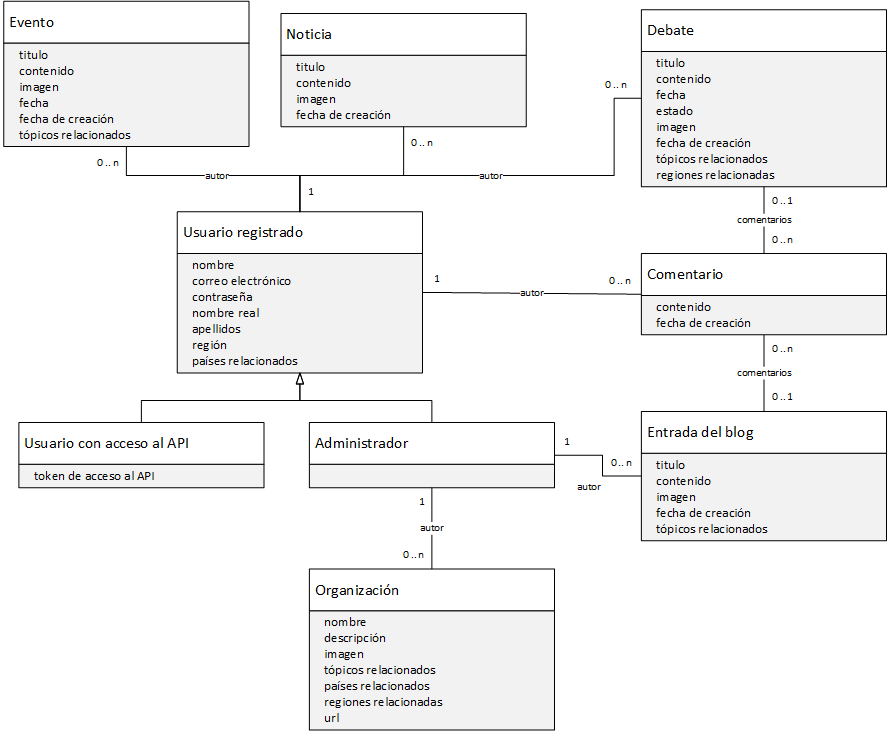
\includegraphics[height=\textwidth]{clases/clases_debate_preliminar}
		\caption{Diagrama de clases preliminares de la zona social}
		\label{fig:clases_preliminares_modelo_debate}
	\end{figure}
\end{landscape}

\subsubsection{Descripción de las clases}
\begin{description}
\item[Usuario registrado]	Representa a los usuarios que tienen una cuenta de usuario y han iniciado sesión en el portal.  Puede crear noticias, eventos, debates y realizar comentarios.  Sus atributos son los siguientes:
							\begin{itemize}
								\item \textbf{Nombre}  Será el nombre con el que el sistema identifica a cada usuario.  El nombre de usuario debe ser único.
								\item \textbf{Correo electrónico}  Será la dirección a la que el sistema enviará los correos electrónicos de contacto, por ejemplo: cuando el usuario solicita una nueva contraseña.  El correo electrónico debe ser único.
								\item \textbf{Contraseña}  Será utilizada para autenticar la identidad del usuario al iniciar sesión en el sistema o al modificar la información de su perfil.
								\item \textbf{Nombre real}  Será el nombre real del usuario, podrá ser visto por otros usuarios al visitar su perfil.
								\item \textbf{Apellidos}  Serán los apellidos reales del usuario, podrán ser vistos por otros usuarios al visitar su perfil.
								\item \textbf{Continente}  Será el continente en el que se encuentra el usuario.  Éste atributo no será obligatorio y podrá estar vacío.
								\item \textbf{Países relacionados}  Serán los países en los que el usuario tiene algún tipo de interés.  Este atributo no será obligatorio y podrá estar vacío.
							\end{itemize}
\item[Usuario con acceso al API]  Representa a los usuarios registrados que tienen capacidad de acceso al API del sistema.  Tienen las mismas capacidades que cualquier usuario registrado.  Además de los atributos de cualquier usuario registrado también tendrán:
							\begin{itemize}
							\item \textbf{Token}  Será la clave con la que el usuario accede al API.  Ésta clave será secreta y no podrá ser vista por ningún otro usuario.
							\end{itemize}
\item[Administrador]  Representa a los usuarios registrados con privilegios de administración en el sistema.  Tendrán los mismos atributos que cualquier otro usuario registrado pero podrán crear, modificar y eliminar cualquier contenido o comentario.
\item[Noticia]  Representa una noticia de interés en la que la fecha no es importante.  Las noticias podrán ser creadas por cualquier usuario registrado.  Sus atributos serán los siguientes:
							\begin{itemize}
							\item \textbf{Título}  Es el título de la noticia.
							\item \textbf{Contenido}  Es el contenido de la noticia.
							\item \textbf{Imagen}  Es una imagen relacionada con el contenido de la noticia.  Éste atributo no será obligatorio y podrá estar vacío.
							\item \textbf{Fecha de creación}  Es la fecha en la que la noticia fue creada.  Este campo es almacenado automáticamente por el sistema.
							\item \textbf{Autor}  Es el usuario registrado que crea la noticia.  Cada noticia tendrá un único autor, pero cada usuario registrado podrá ser autor de múltiples noticias.
							\end{itemize}
\item[Evento]  Representa una situación o noticia que tendrá lugar en un determinado momento del tiempo.  Los eventos podrán ser creados por cualquier usuario registrado.  Sus atributos serán los siguientes:
							\begin{itemize}
							\item \textbf{Título}  Es el título del evento.
							\item \textbf{Contenido}  Es el contenido del evento, donde se explica toda la información necesaria.
							\item \textbf{Imagen}  Es una imagen relacionada con el contenido del evento.  Éste atributo no será obligatorio y podrá estar vacío.
							\item \textbf{Fecha}  Será la fecha en la que el evento tendrá lugar.
							\item \textbf{Fecha de creación}  Es la fecha en la que el evento fue creado.  Este campo es almacenado automáticamente por el sistema.
							\item \textbf{Tópicos relacionados}  Serán los tópicos relacionados con el contenido del evento.  Los tópicos servirán como metainformación sobre el contenido y ayudarán a enriquecer los resultados de la búsqueda.
							\item \textbf{Autor}  Es el usuario registrado que crea el evento.  Cada evento tendrá un único autor, pero cada usuario registrado podrá ser autor de múltiples eventos.
							\end{itemize}
\item[Debate]  Representa un tema u opinión en el que se quiere permitir la participación de los usuarios.  Sus atributos serán los siguientes:
							\begin{itemize}
							\item \textbf{Título}  Es el título del debate.
							\item \textbf{Contenido}  Es el contenido del debate, donde se expone el tema a tratar por los usuarios.
							\item \textbf{Fecha}  Será la fecha o periodo de fechas en las que el debate tendrá lugar.
							\item \textbf{Estado}  Es el estado en el que se encuentra el debate.  Los posibles estados son ``abierto'', ``cerrado'' o ``próximamente''.
							\item \textbf{Imagen}  Es una imagen relacionada con el contenido del debate.  Éste atributo no será obligatorio y podrá estar vacío.
							\item \textbf{Fecha de creación}  Es la fecha en la que el debate fue creado.  Este campo es almacenado automáticamente por el sistema.
							\item \textbf{Tópicos relacionados}  Serán los tópicos relacionados con el contenido del debate.  Los tópicos servirán como metainformación sobre el contenido y ayudarán a enriquecer los resultados de la búsqueda.
							\item \textbf{Regiones relacionadas}  Serán las regiones relacionadas con el debate o a las que éste hace referencia.  Al igual que los tópicos, las regiones servirán como metainformación sobre el contenido y ayudarán a enriquecer los resultados de la búsqueda.
							\item \textbf{Autor}  Es el usuario registrado que crea el debate.  Cada debate tendrá un único autor, pero cada usuario registrado podrá ser autor de múltiples debates.
							\item \textbf{Comentarios}  Son los comentarios que los usuarios realizan en el debate.  Cada debate podrá tener múltiples comentarios, pero cada comentario sólo podrá pertenecer a un debate.
							\end{itemize}
\item[Entrada del blog]  Representa una entrada en el blog oficial de Land Portal.  Las entradas en el blog sólo pueden ser creadas por los administadores.  Sus atributos son los siguientes:
							\begin{itemize}
							\item \textbf{Título}  Es el título de la entrada.
							\item \textbf{Contenido}  Es el contenido de la entrada.
							\item \textbf{Imagen}  Es una imagen relacionada con el contenido de la entrada.  Éste atributo no será obligatorio y podrá estar vacío.
							\item \textbf{Fecha de creación}  Es la fecha en la que la entrada fue creada.  Este campo es almacenado automáticamente por el sistema.
							\item \textbf{Tópicos relacionados}  Serán los tópicos relacionados con el contenido de la entrada.  Los tópicos servirán como metainformación sobre el contenido y ayudarán a enriquecer los resultados de la búsqueda.
							\item \textbf{Autor}  Es el administrador que crea la entrada.  Cada entrada tendrá un único autor, pero cada administrador podrá ser autor de múltiples entradas.
							\item \textbf{Comentarios}  Son los comentarios que los usuarios realizan en la entrada.  Cada entrada podrá tener múltiples comentarios, pero cada comentario sólo podrá pertenecer a una entrada.
							\end{itemize}
\item[Comentario]  Representa la opinión que un usuario hace pública en un debate o una entrada del blog:
							\begin{itemize}
							\item \textbf{Contenido}  Es el contenido del comentario.
							\item \textbf{Fecha de creación}  Es la fecha en la que el comentario fue creado.  Este campo es almacenado automáticamente por el sistema.
							\item \textbf{Autor}  Es el usuario registrado que crea el comentario.  Cada comentario tiene un autor, pero un usuario registrado puede ser autor de múltiples comentarios.
							\end{itemize}
\end{description}


\section{Análisis de interfaces de usuario}
\label{analisis_interfaces_usuario}
En esta sección se realizará una primera aproximación a la posible interfaz que tendrá el portal, detallando y explicando las vistas que la conforman.  A continuación se mostrarán los \textit{mockups} de la interfaz y se explicará cada uno de ellos.



\subsection{Interfaz de la zona de datos}
Como se ha mencionado en la sección ``\nameref{definicion_sistema}'' perteneciente al capítulo \ref{chapter04}, la interfaz de zona de datos (o \textit{LandBook}) queda fuera del alcance de éste proyecto, por lo que no se mostrarán \textit{mockups} para dicha sección.



\subsection{Interfaz de administración}
La interfaz de administración será directamente proveída por el gestor de contenidos que, como se ha mencionado en la sección ``\nameref{chapter02:alternativas_seleccionadas}'' perteneciente al capítulo \ref{chapter02}, será Drupal.  Por esta razón no se mostrarán \textit{mockups} pertenecientes a dicha interfaz.



\subsection{Interfaz de la zona social}
A continuación se mostrarán los \textit{mockups} de la zona social (o \textit{LandDebate}).


\subsubsection{Vista del blog del Land Portal}
\label{chapter04:mockup_blog}
La figura \ref{fig:mockup_blog} muestra el \textit{mockup} de la vista que conformará el blog del nuevo Land Portal.

Ésta pantalla mostrará las entradas del blog ordenadas de más a menos reciente.  Las tres entradas más recientes se destacarán sobre el resto, e incluirán:
\begin{itemize}
	\item Título de la entrada, enlazado a la vista de detalle de la propia entrada.
	\item Imagen de la entrada.
	\item Autor y fecha en la que la entrada fue añadida al blog.
	\item Tópicos relacionados.  Al pulsar en un tópico, se accederá a una vista en la que se mostrarán todos los contenidos del portal relacionados con dicho tópico.
	\item Resumen del contenido de la entrada.
\end{itemize}

\begin{figure}[h]
	\centering
	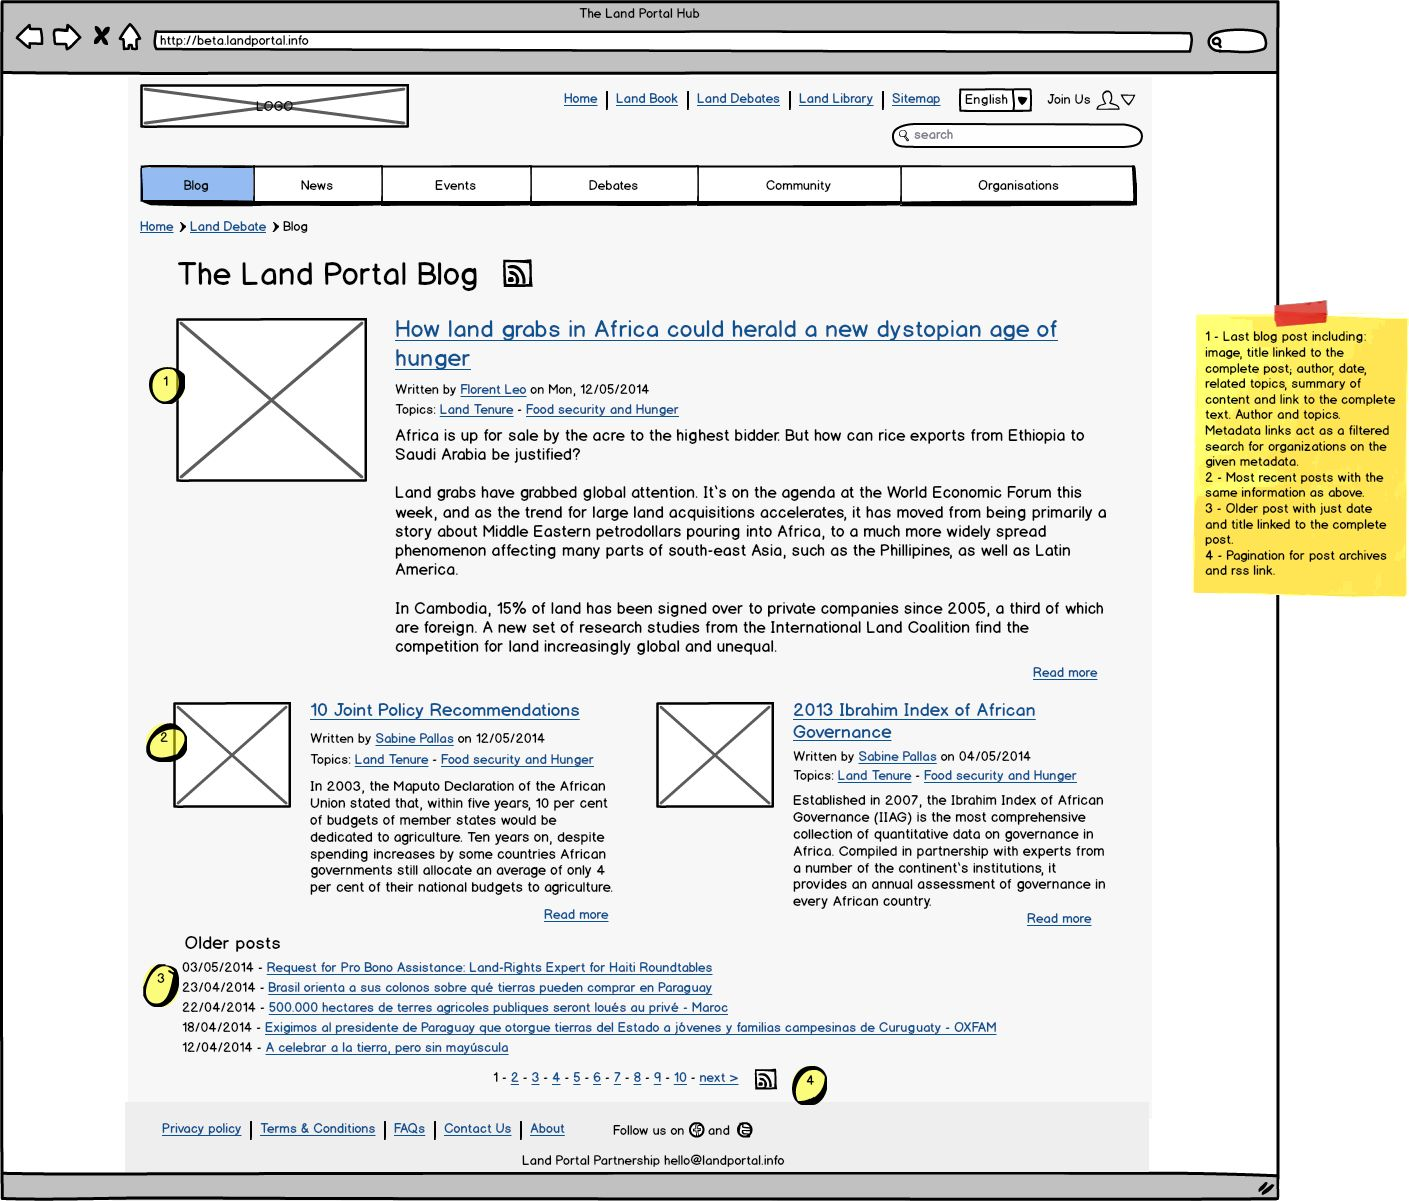
\includegraphics[width=\textwidth]{mockups/blog}
	\caption{\textit{Mockup} de la vista del blog del Land Portal}
	\label{fig:mockup_blog}
\end{figure}

Las entradas anteriores tendrán menos énfasis en la vista, y sólo estarán representadas por su título y la fecha en la que han sido creadas.  Además también se incluirá un paginador para recorrer las noticias anteriores y un enlace al \textit{feed} RSS\footnote{El feed RSS permite suscribirse a las últimas entradas del blog utilizando un lector de feeds RSS como Feedly, Newsvibe o Digg Reader y obtener las actualizaciones de forma automática en el lector sin necesidad de acceder al portal.} donde también se encontrarán las últimas noticias.


\subsubsection{Vista de detalle de una entrada del blog}
\label{chapter04:mockup_blog_entry}
La figura \ref{fig:mockup_entrada_blog} muestra el \textit{mockup} de la vista de detalle de una entrada del blog.  Esta vista incluirá:
\begin{itemize}
	\item Título de la entrada
	\item Autor y fecha de creación de la entrada
	\item Tópicos relacionados.  Como ya se ha explicado anteriormente, al pulsar sobre un tópico, el sistema cargará una vista con todos los contenidos relacionados con dicho tópico.
	\item Contenido de la entrada
	\item Imagen relacionada
	\item Botones destinados a compartir el contenido de la entrada en redes sociales como Twitter o Facebook.
\end{itemize}

En la zona inferior de la vista se incluirá la sección de comentarios.  En esta sección los usuarios podrán participar y dar su opinión a cerca del tema tratado en la entrada del blog.  Cada comentario mostrará su contenido, su autor y la fecha en al que fue creado.  Los comentarios se mostrarán ordenados según su fecha de creación.

\begin{figure}[h]
	\centering
	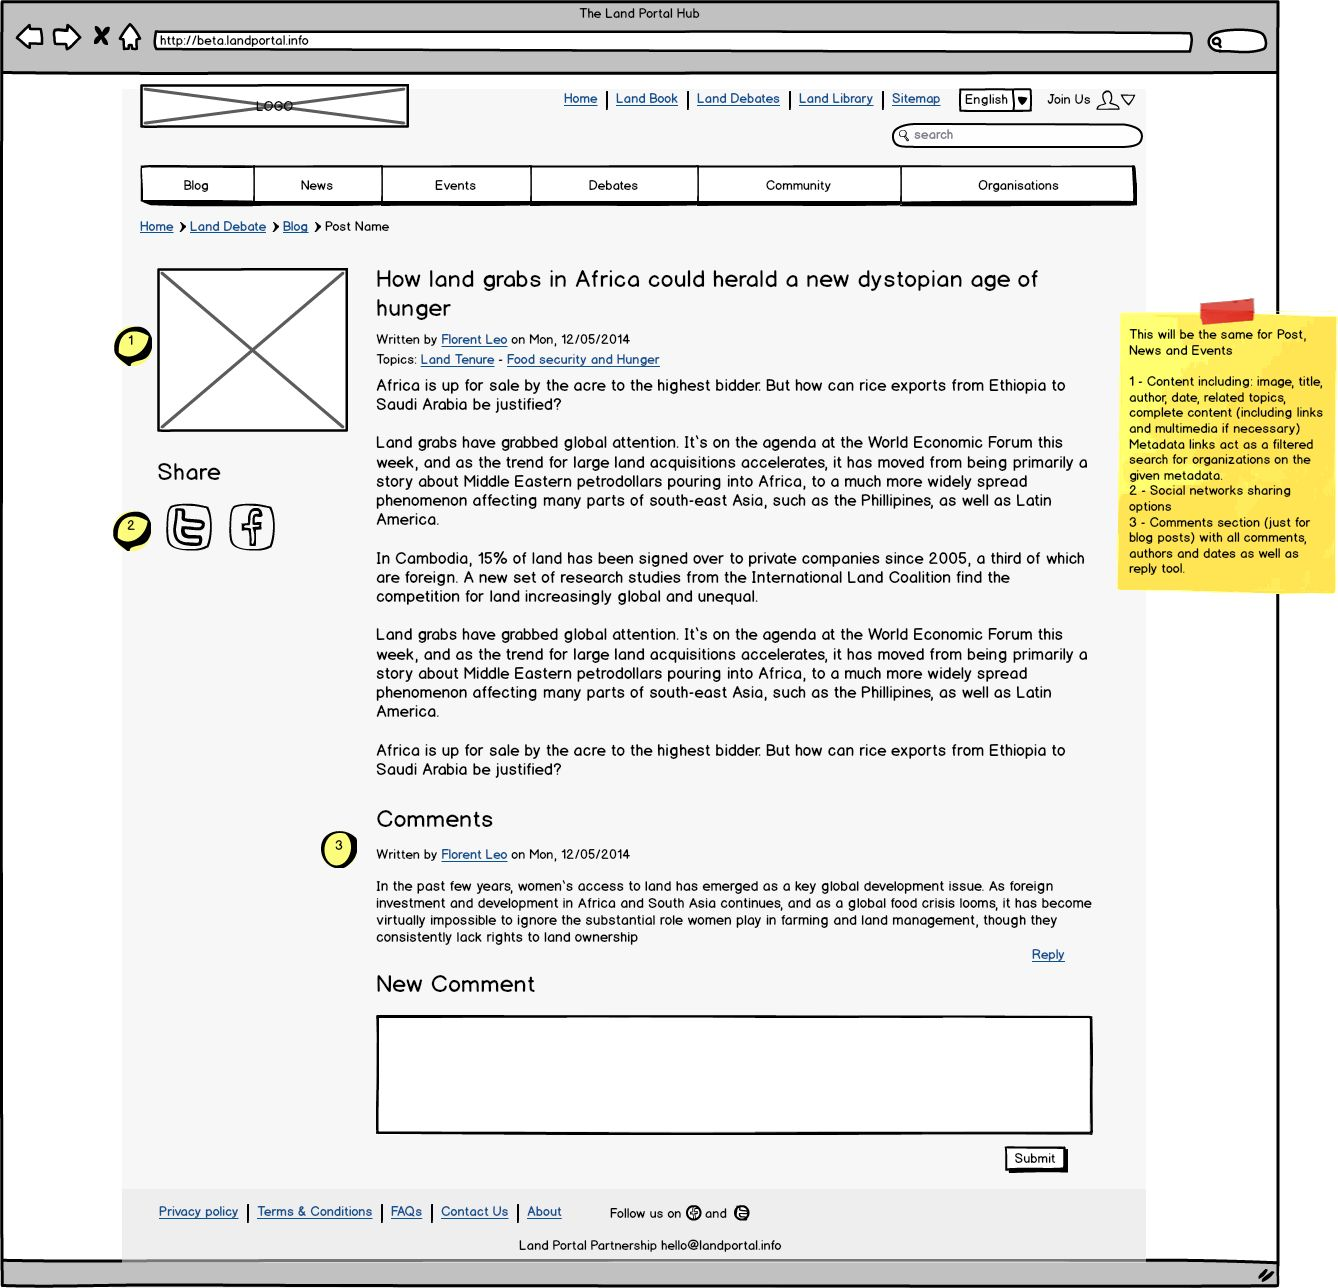
\includegraphics[width=\textwidth]{mockups/post-new-event}
	\caption{\textit{Mockup} de la vista de detalle de una entrada del blog}
	\label{fig:mockup_entrada_blog}
\end{figure}


\subsubsection{Vista de eventos}
\label{chapter04:mockup_eventos}
La figura \ref{fig:mockup_eventos} muestra el \textit{mockup} de la vista de eventos del nuevo Land Portal.  Los dos eventos más recientes se destacarán sobre el resto e incluirán:
\begin{itemize}
	\item Título del evento, enlazado a la vista de detalle del propio evento.
	\item Imagen del evento.
	\item Autor y fecha en la que el evento fue creado.
	\item Tópicos relacionados.  Al pulsar en un tópico, se accederá a una vista en la que se mostrarán todos los contenidos del portal relacionados con dicho tópico.
	\item Resumen del contenido del evento.
\end{itemize}
De forma similar a como sucede en el blog, los eventos anteriores tendrán menos importancia en la vista, y únicamente se mostrarán con su título y la fecha en la que el evento tiene lugar.  También al igual que el blog, se incluye un paginador y un enlace al \textit{feed} RSS donde también se encontrarán los últimos eventos.

Un añadido especial de ésta vista es un calendario que mostrará resaltados los días en los que tiene lugar algún evento.
\begin{figure}[h]
	\centering
	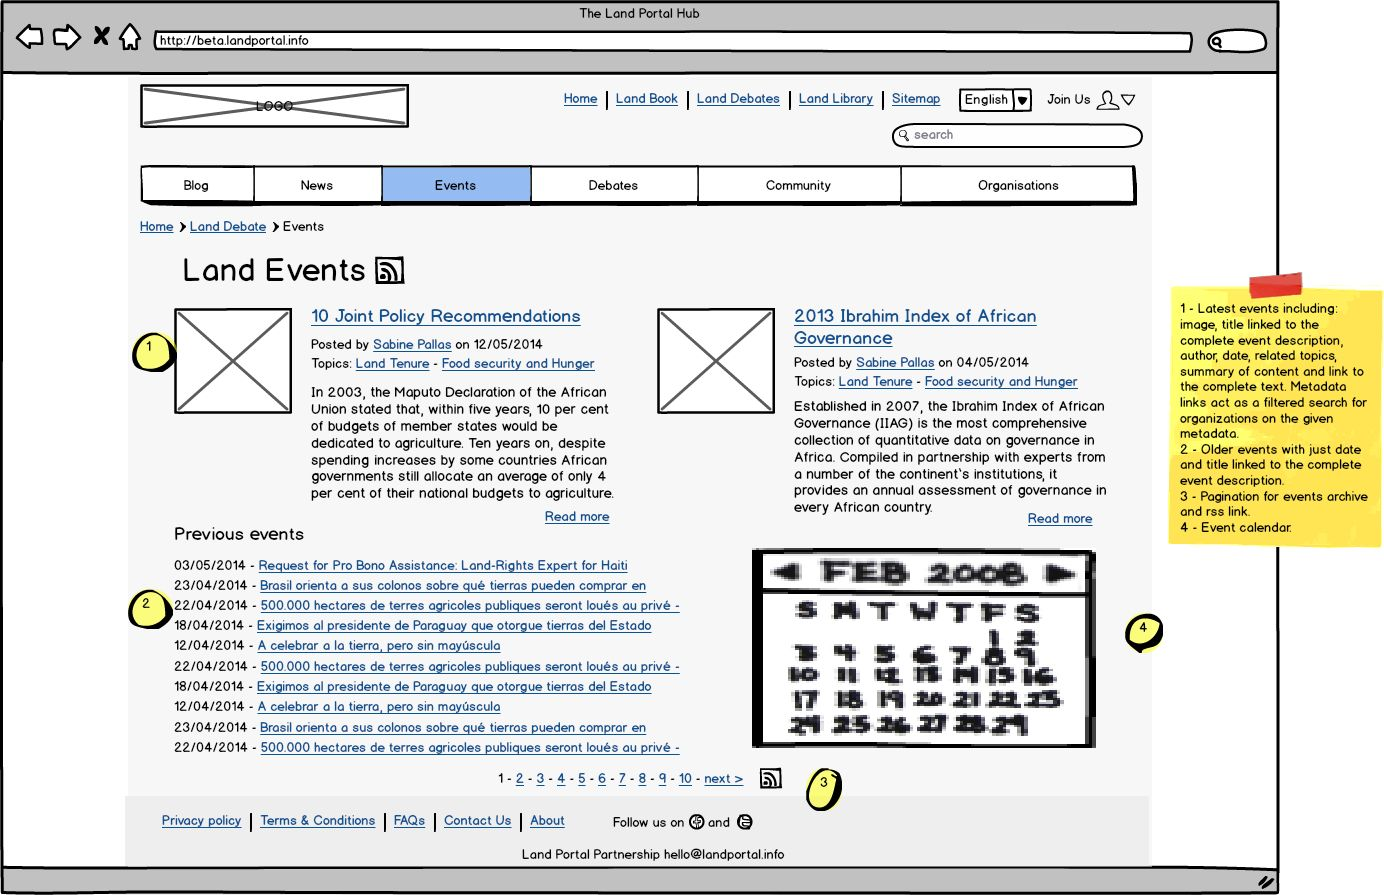
\includegraphics[width=\textwidth]{mockups/events}
	\caption{\textit{Mockup} de la vista de eventos}
	\label{fig:mockup_eventos}
\end{figure}


\subsubsection{Vista de noticias}
\label{chapter04:mockup_noticias}
La figura \ref{fig:mockup_noticias} muestra el \textit{mockup} de la vista de noticias del nuevo Land Portal.  Las cuatro noticias más recientes se destacarán sobre el resto e incluirán:
\begin{itemize}
	\item Título de la noticia, enlazado a la vista de detalle de la propia noticia.
	\item Imagen de la noticia
	\item Resumen del contenido de la noticia.
\end{itemize}
Al igual que en la vista de eventos y del blog, las noticias anteriores sólo mostrarán su título y fecha de creación.  También se incluirán, de la misma forma que las vistas anteriores, un paginador y un enlace al \textit{feed} RSS con las últimas noticias.

Una característica especial de ésta vista será que en la parte izquierda de la misma se mostrarán las últimas actualizaciones de la cuenta de Twitter de Land Portal\footnote{La cuenta oficial de Land Portal se puede ver en \url{https://twitter.com/landportal}}.  Para incluír éste componente se utilizará la capacidad de generación de \textit{widgets} de Twitter.
\begin{figure}[h]
	\centering
	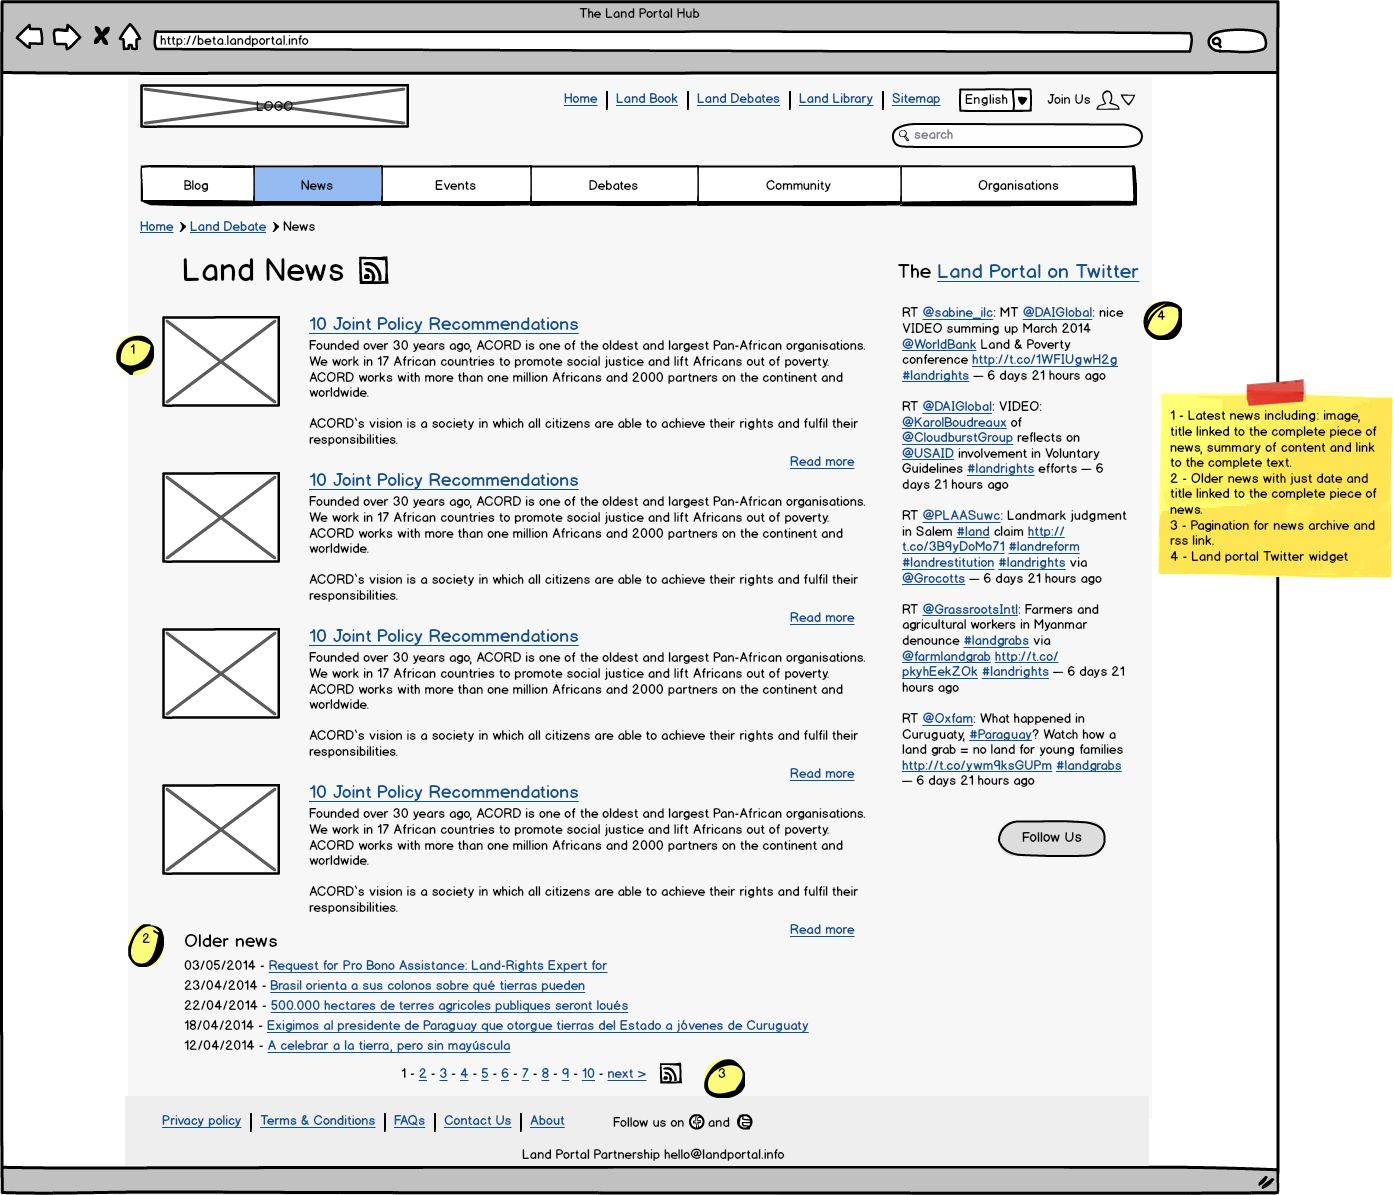
\includegraphics[width=\textwidth]{mockups/news}
	\caption{\textit{Mockup} de la vista de noticias}
	\label{fig:mockup_noticias}
\end{figure}


\subsubsection{Vista de debates}
La figura \ref{fig:mockup_debates} muestra el \textit{mockup} de la vista de debates del nuevo Land Portal.  Ésta vista tiene una importancia clave dentro de la zona social, puesto que los debates serán el principal punto en el que los usuarios participen e intercambien opiniones.  Los debates que no estén cerrados se destacarán sobre el resto e incluirán:
\begin{itemize}
	\item Título del debate, enlazado a la vista de detalle del mismo.
	\item Autor del debate.
	\item Tópicos relacionados.  Al pulsar en un tópico, se accederá a una vista en la que se mostrarán todos los contenidos del portal relacionados con dicho tópico.
	\item Resumen del contenido del debate.
	\item Imagen del debate.
	\item Fecha o fechas en las que el debate tendrá lugar.
	\item Estado del debate.
\end{itemize}

De forma similar a las vistas anteriores, también se incluirán los debates anteriores (en este caso los debates ya cerrados) únicamente con su título y la fecha en la qu ese han creado y un enlace al \textit{feed} RSS de la sección de debates.

Puesto que, como se ha dicho anteriormente, ésta vista juega un papel clave fomentando la participación de los usuarios en el portal.  Por ello, en la zona derecha se mostrarán los últimos comentarios que los usuarios hayan realizado en algún debate.  Cada comentario incluirá:
\begin{itemize}
	\item Fecha de creación del comentario.
	\item Autor del comentario.
	\item Título del comentario enlazado al propio comentario dentro de la vista de detalle del debate.
	\item Resumen del contenido del comentario.
\end{itemize}
\begin{figure}[h]
	\centering
	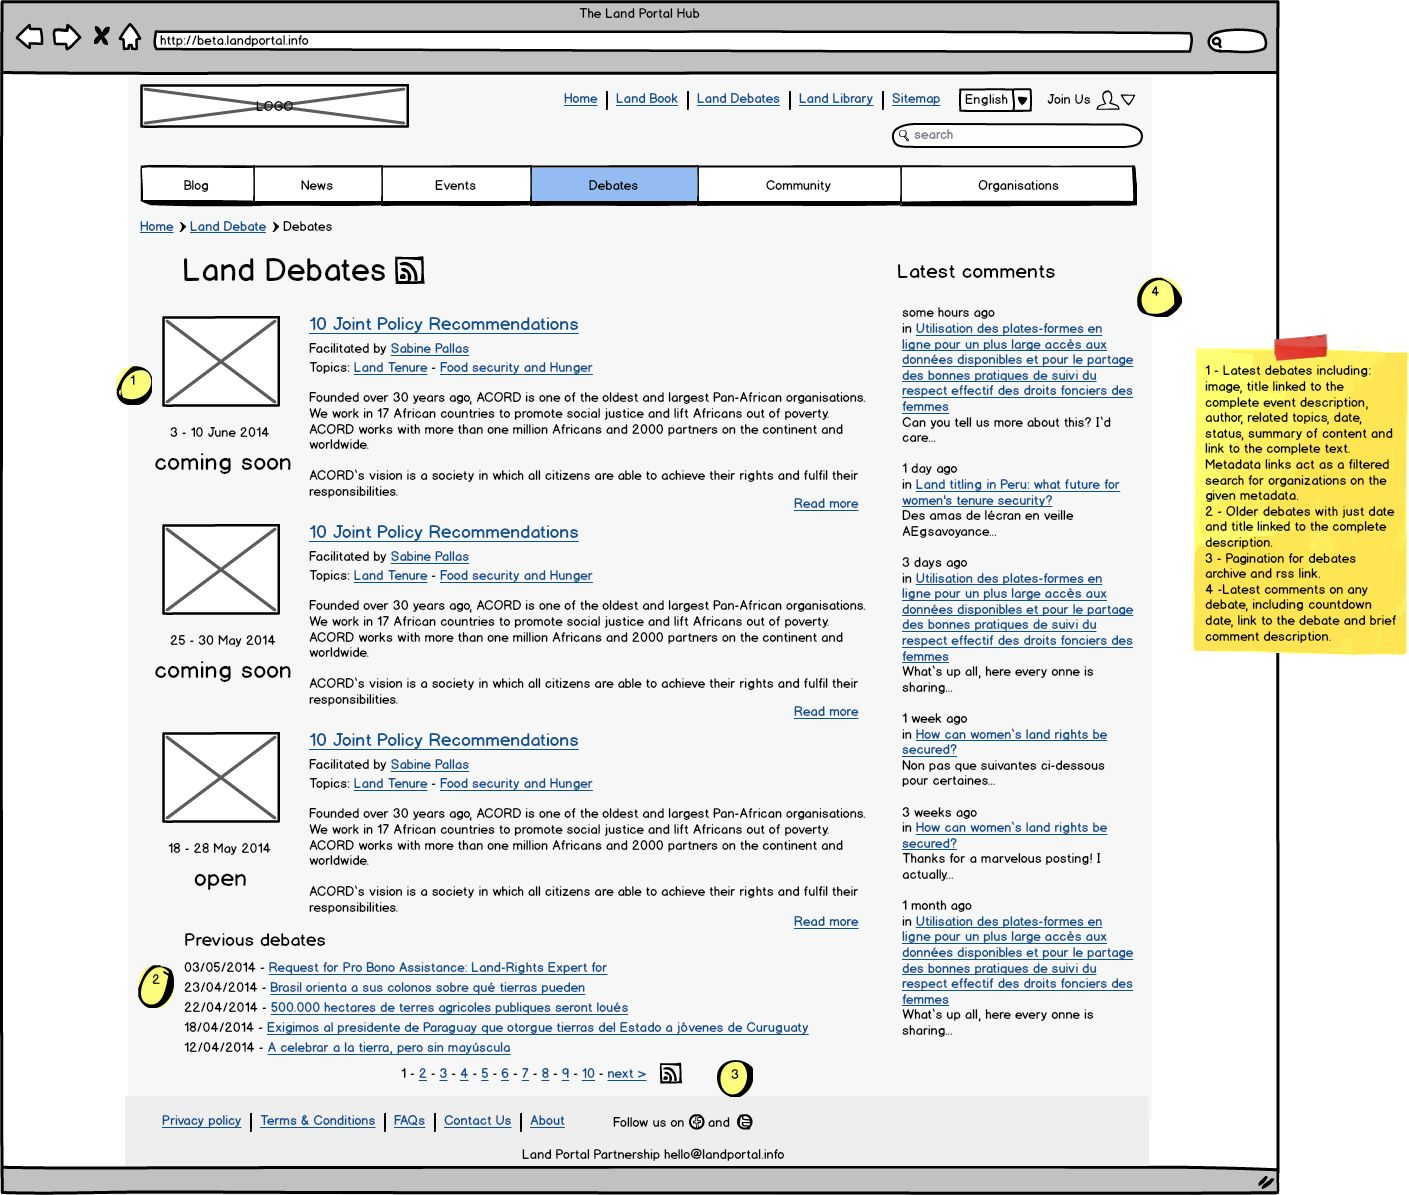
\includegraphics[width=\textwidth]{mockups/debates}
	\caption{\textit{Mockup} de la vista de debates}
	\label{fig:mockup_debates}
\end{figure}


\subsubsection{Vista de detalle de un debate}
La figura \ref{fig:mockup_debate} muestra el \textit{mockup} de la vista de detalle de un debate.  Al igual que la vista de debates descrita anteriormente, esta vista juega también un rol clave para fomentar la participación de los usuarios en el portal.

La vista incluirá toda la información del debate, incluyendo:
\begin{itemize}
	\item Título del debate
	\item Tópicos y países relacionados
	\item Idioma en el que tendrá lugar el debate
	\item Contenido del debate
	\item Imagen del debate
	\item Estado
	\item Autor del debate
\end{itemize}

En la parte inferior de esta vista se ubicará la sección de comentarios.  El comportamiento de la sección de comentarios variará en función del estado del debate.  Cuando el debate esté abierto, los usuarios podrán participar e incluir nuevos comentarios o  responder a los comentarios ya existentes.  Cuando el debate esté cerrado se mostrarán los comentarios existentes, pero no se permitirá añadir ningún comentario nuevo.  Los comentarios se mostrarán ordenados según su fecha de creación.

Para reforzar la función social de esta vista, se incluirán también una serie de botones que permitirán compartir el debate en redes sociales como Twitter o Facebook.  Al mismo tiempo, en la parte derecha de la vista se mostrarán los últimos comentarios relacionados en la red social Twitter.

\begin{figure}[h]
	\centering
	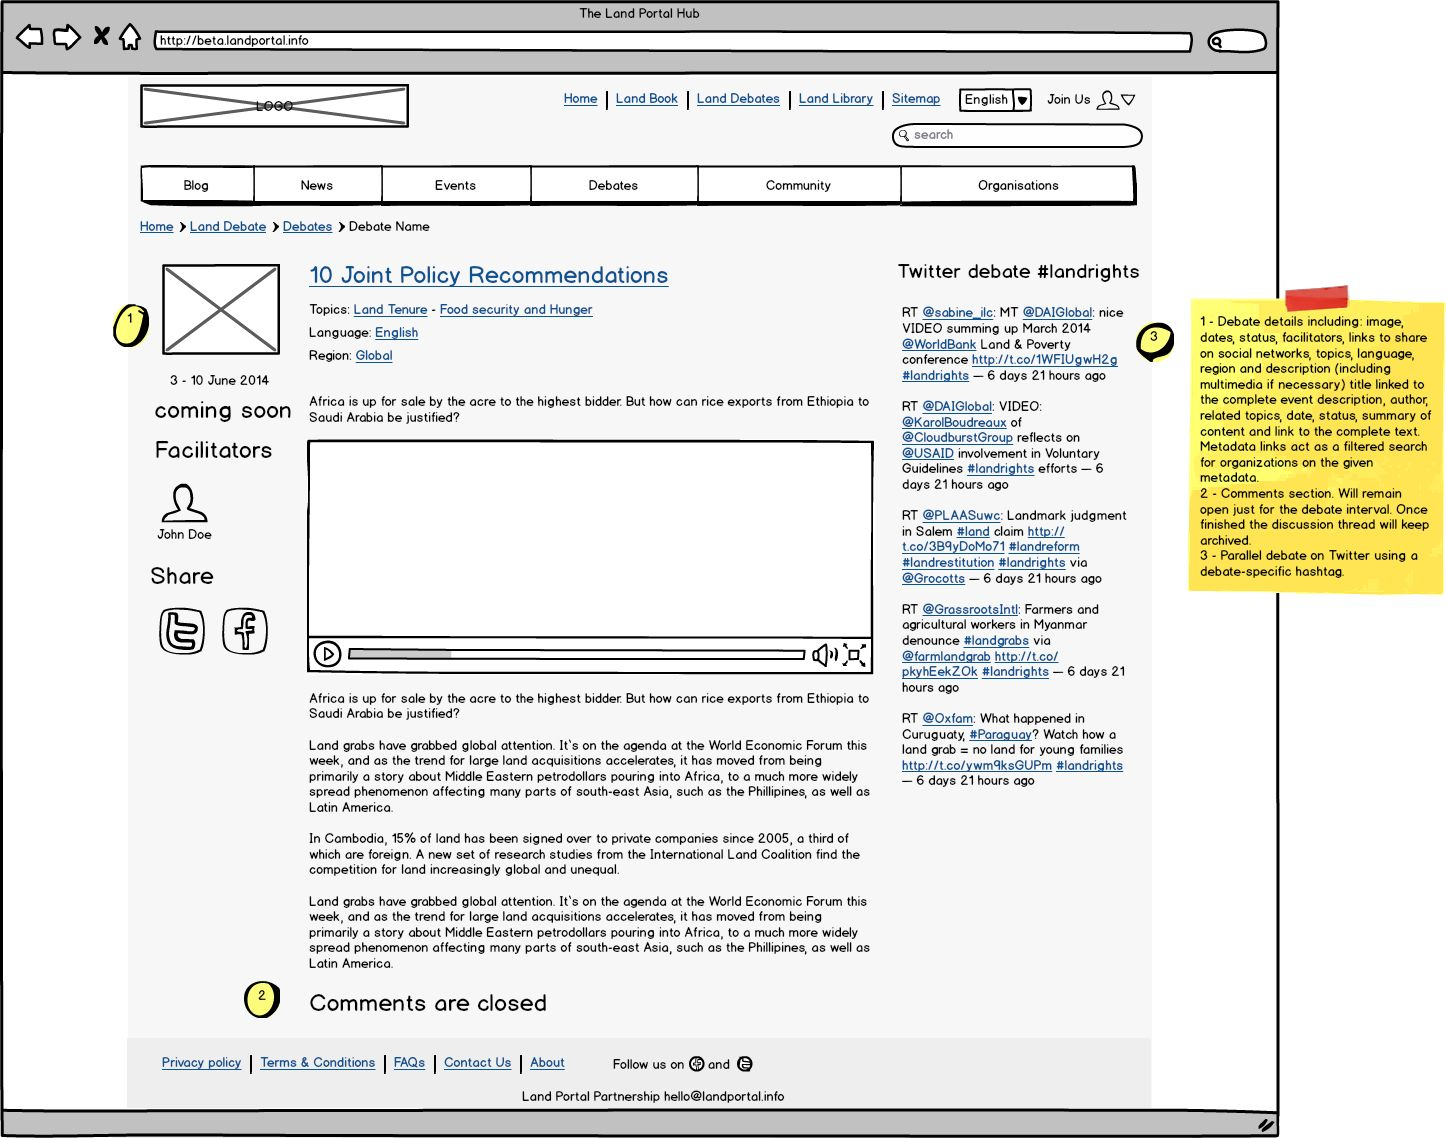
\includegraphics[width=\textwidth]{mockups/debate}
	\caption{\textit{Mockup} de la vista de detalle de un debate}
	\label{fig:mockup_debate}
\end{figure}


\subsubsection{Vista de detalle de un evento y de una noticia}
\label{mockup_noticia_evento}
Las vistas del detalle de un evento y una noticia serán similares a la vista de detalle de una entrada en el blog, el \textit{mockup} para dicha vista puede verse en la figura \ref{fig:mockup_entrada_blog}.

La única diferencia de estas vistas respecto a la vista de detalle de una entrada del blog será que ni los eventos ni las noticias tendrán sección de comentarios.


\subsubsection{Vista de organizaciones}
La figura \ref{fig:mockup_organizaciones} muestra el \textit{mockup} de la vista de organizaciones. Esta vista mostrará las organizaciones existentes en el portal en forma de parrilla o \textit{grid}, en la que cada organización mostrará su imagen y su nombre, ambos enlazados a la vista de detalle de dicha organización.

En la zona derecha de la vista se incluirán una serie de controles con los que será posible buscar organizaciones determinadas.  Además, siguiendo con la tónica social del portal ya mencionada anteriormente, se mostrará un \textit{widget} con el contenido de la comunidad de Land Portal en la red social Facebook\footnote{La página oficial de Land Portal en Facebook puede verse en la siguiente dirección: \url{https://www.facebook.com/landportal}}.

\begin{figure}[h]
	\centering
	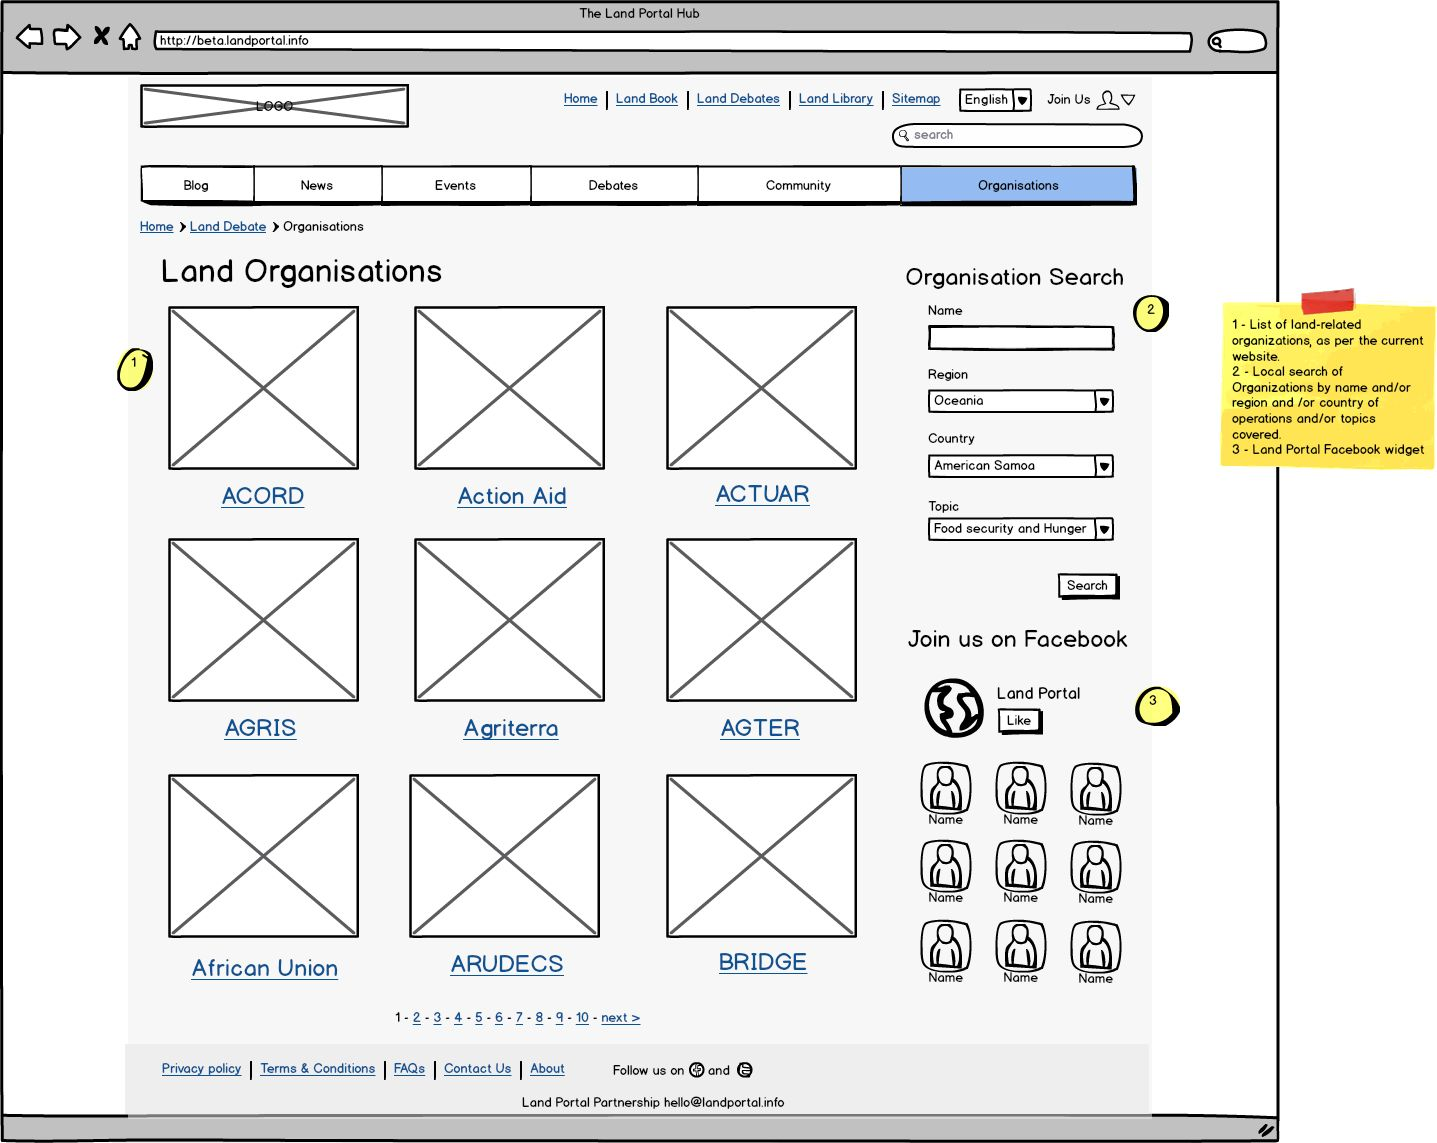
\includegraphics[width=\textwidth]{mockups/organisations}
	\caption{\textit{Mockup} de la vista de organizaciones}
	\label{fig:mockup_organizaciones}
\end{figure}


\subsubsection{Vista de detalle de una organización}
La figura \ref{fig:mockup_organizacion} muestra el \textit{mockup} de la vista de detalle de una organización. Esta vista mostrará las organizaciones existentes en el portal en forma de parrilla o \textit{grid}, en la que cada organización mostrará su imagen y su nombre, ambos enlazados a la vista de detalle de dicha organización.

Esta vista mostrará la imagen, el nombre y una descripción de la organización.  Además también se incluirá un enlace a la página web de dicha organización.  En la parte derecha de la vista se mostrarán los metadatos de la organización, como: el área y los países en los que opera o los tópicos relacionados.  Al pulsar en cualquier término de estos metadatos el sistema cargará una vista que mostrará todo el contenido del portal relacionado con dicho término.

\begin{figure}[h]
	\centering
	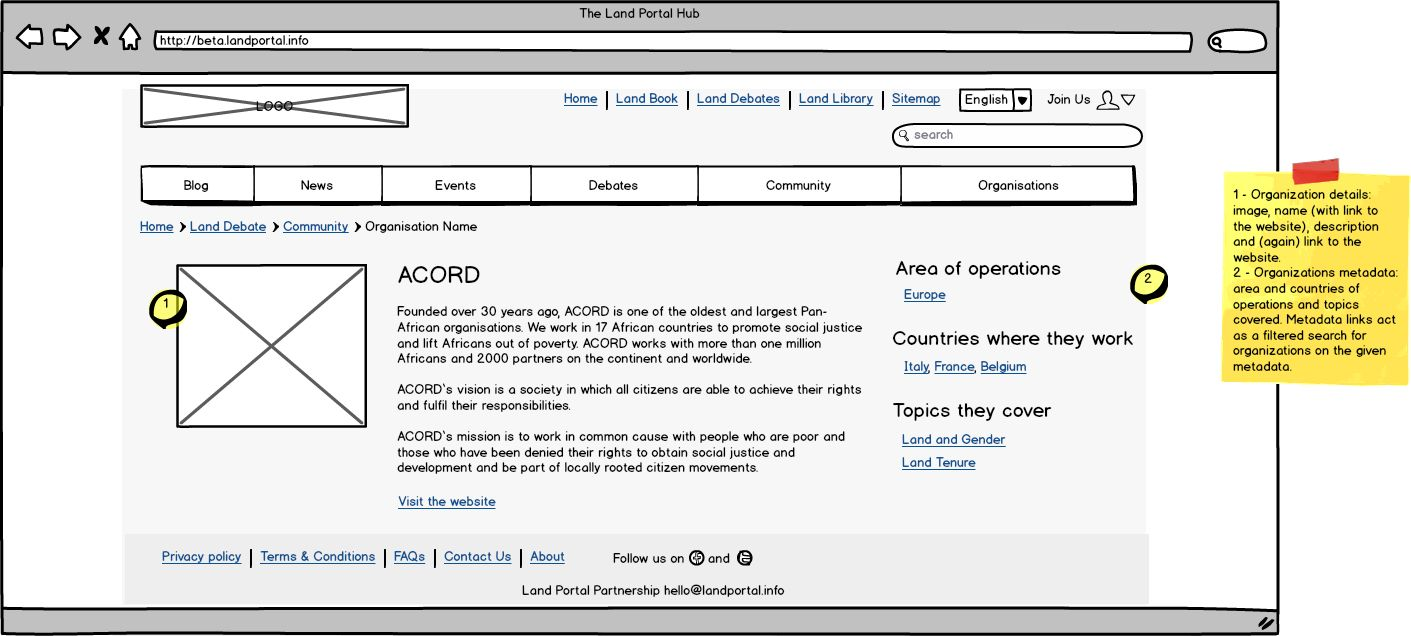
\includegraphics[width=\textwidth]{mockups/organisation}
	\caption{\textit{Mockup} de la vista de detalle de una organización}
	\label{fig:mockup_organizacion}
\end{figure}


\subsubsection{Vista de comunidad}
La vista de la comunidad será similar a la vista de organizaciones, la cual se puede ver en la figura \ref{fig:mockup_organizaciones}.  Las únicas diferencias respecto a la vista de organizaciónes serán:
\begin{itemize}
	\item En lugar de mostrar las organizaciones del portal, esta vista mostrará en una parrilla o \textit{grid} los usuarios registrados en el portal.
	\item En la zona derecha (además del formulario de búsqueda y el \textit{widget} de la red social Facebook) se incluirá un botón para facilitar el registro de nuevos usuarios.
\end{itemize}

\subsubsection{Vista de login}
La figura \ref{fig:mockup_login} muestra el \textit{mockup} de la vista de login. Esta vista permitirá que los usuarios inicien sesión en el portal.  La vista de login contará con un formulario donde el usuario introducirá su nombre de usuario o email y su contraseña para iniciar sesión en el sistema.  También existirá un enlace mediante el cual un usuario podrá solicitar una nueva contraseña en caso de haber olvidado la suya.

Además, siguiendo con la línea social del portal, se incluyen dos botones destinados a iniciar sesión en el sistema utilizando las redes sociales Twitter y Facebook.

\begin{figure}[h]
	\centering
	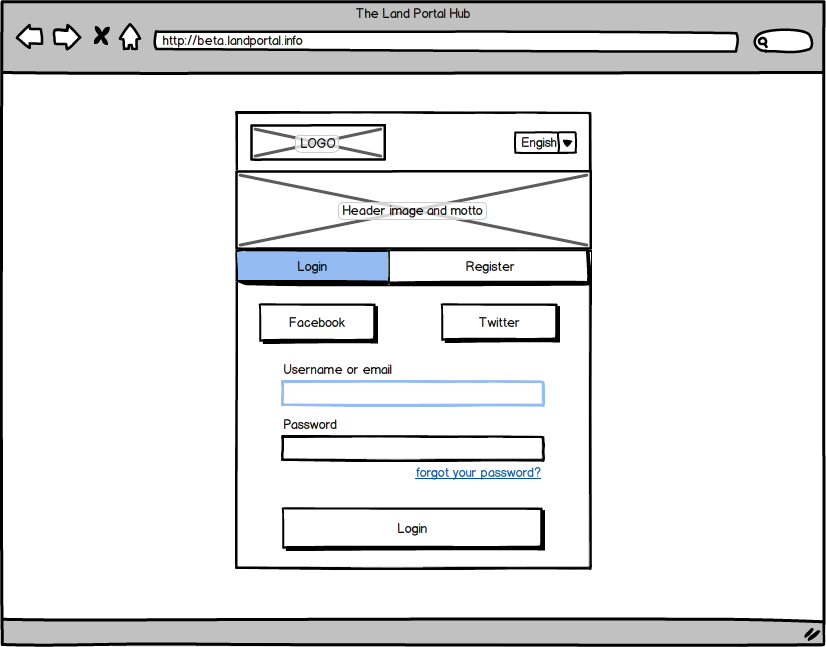
\includegraphics[width=\textwidth]{mockups/login}
	\caption{\textit{Mockup} de la vista de login}
	\label{fig:mockup_login}
\end{figure}


\subsubsection{Vista de registro}
La figura \ref{fig:mockup_registro} muestra el \textit{mockup} de la vista de registro. Esta vista permitirá a los usuarios crear una nueva cuenta en el sistema.  La vista de registro contará con un formulario donde el usuario introducirá su nombre de usuario, su email, su nombre y apellidos y los países y continentes en los que esté interesado. Los campos obligatorios para crear una nueva cuenta de usuario están marcados con un asterisco.  

El botón de registro creará la nueva cuenta en el sistema con un estado ``desactivado'', a la espera de ser activada por un administrador.

\begin{figure}[h]
	\centering
	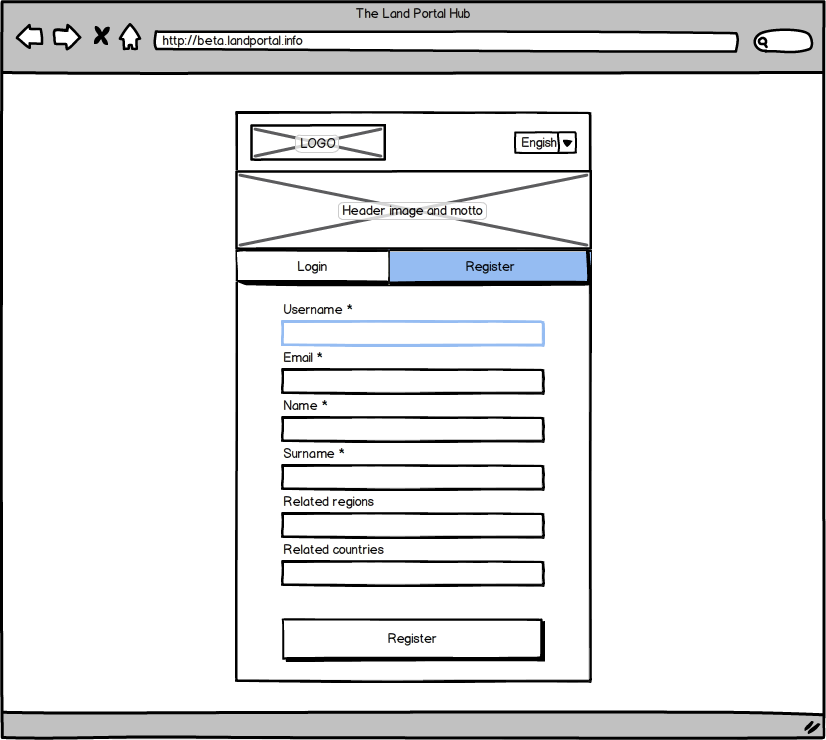
\includegraphics[width=\textwidth]{mockups/register}
	\caption{\textit{Mockup} de la vista de registro}
	\label{fig:mockup_registro}
\end{figure}




\subsubsection{Vista de búsqueda}
La figura \ref{fig:mockup_buscar} muestra el \textit{mockup} de la vista de búsqueda.  Esta vista permitirá a los usuarios buscar cualquier tipo de contenido en el portal.   Al pulsar sobre cada resultado de búsqueda el usuario accederá a la vista de detalle del mismo.

Como se puede ver en la imagen, cada resultado de la búsqueda se presentará de una forma diferente y tendrá asociada una etiqueta en la que se indica el tipo de contenido al que pertenece.  Al pulsar en esta etiqueta, el sistema cargará la vista correspondiente a cada tipo de contenido.

\begin{figure}[h]
	\centering
	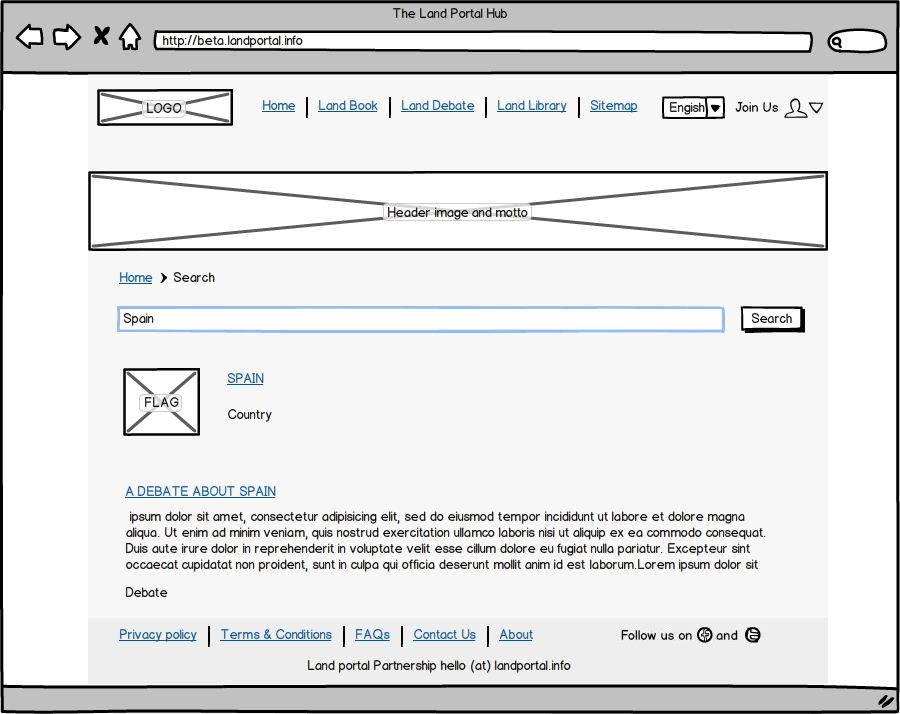
\includegraphics[width=\textwidth]{mockups/search}
	\caption{\textit{Mockup} de la vista de busqueda}
	\label{fig:mockup_buscar}
\end{figure}

\chapter{Diseño del sistema}
\label{chapter05}
\section{Arquitectura del sistema}
\label{arquitectura_sistema}
En ésta sección se explicará en detalle el diseño estructural del sistema.  Cada una de las partes a detallar se dividirá a su vez en varias partes:
\begin{itemize}
	\item Se incluirá un diagrama que muestre de forma gráfica el diseño del componente y sus subcomponentes
	\item Se dará una explicación textual de los diferentes subcomponentes y las tareas que realizan
	\item Se dará una explicación textual sobre cómo se relacionan los subcomponentes entre sí
	\item Se describirá de forma detallada las interfaces y puertos utilizadas por los subcomponentes.  Las interfaces y puertos se dividirán en tablas por componentes para hacer más sencilla su lectura.	Cada entrada constará de los siguientes apartados:
	\begin{itemize}
		\item \textbf{Interfaz}.  Será el nombre que recibe el puerto/interfaz en el diagrama de componentes.
		\item \textbf{Tipo}.  El tipo de la interfaz/puerto será \textit{proveído} cuando se exponga una interfaz para su uso por parte de otro componente, o \textit{requerido} cuando se utilice una interfaz expuesta por otro componente.
		\item \textbf{Tecnología}.  Indica el tipo de tecnología de la interfaz/puerto.
		\item \textbf{Propiedades}.  Explica brevemente el objetivo de la interfaz/puerto.
	\end{itemize}
\end{itemize}

Es importante destacar que ésta sección se centrará en el subsistema de datos puesto que, como ya se ha mencionado en la sección \nameref{identificacion_subsistemas} perteneciente al capítulo \ref{chapter04}, los subsistemas pertenecientes a la zona social (subsistema de gestión de usuarios, eventos, noticias, debates, entradas del blog y comentarios) delegan su funcionalidad en componentes ya implementados por el gestor de contenidos.  De la misma forma, el subsistema de búsqueda delega su funcionalidad principal en el servidor de búsqueda.

\subsection{Vista del sistema}
\label{vista_sistema}
A continuación se detallará la estructura completa del sistema que forma el nuevo \textit{Land Portal}.  A pesar de que varios de los componentes que se verán aquí quedan fuera del ámbito de este proyecto, se ha decidido incluir esta vista para proveer de un contexto que permita al lector comprender en qué parte del sistema se situarán las vistas posteriores.

\subsubsection{Diagrama de componentes}
La figura \ref{fig:diagrama_componentes_sistema} muestra el diagrama de todos los componentes que conforman el nuevo \textit{Land Portal}.
\begin{landscape}
	\begin{figure}[ht]
		\centering
		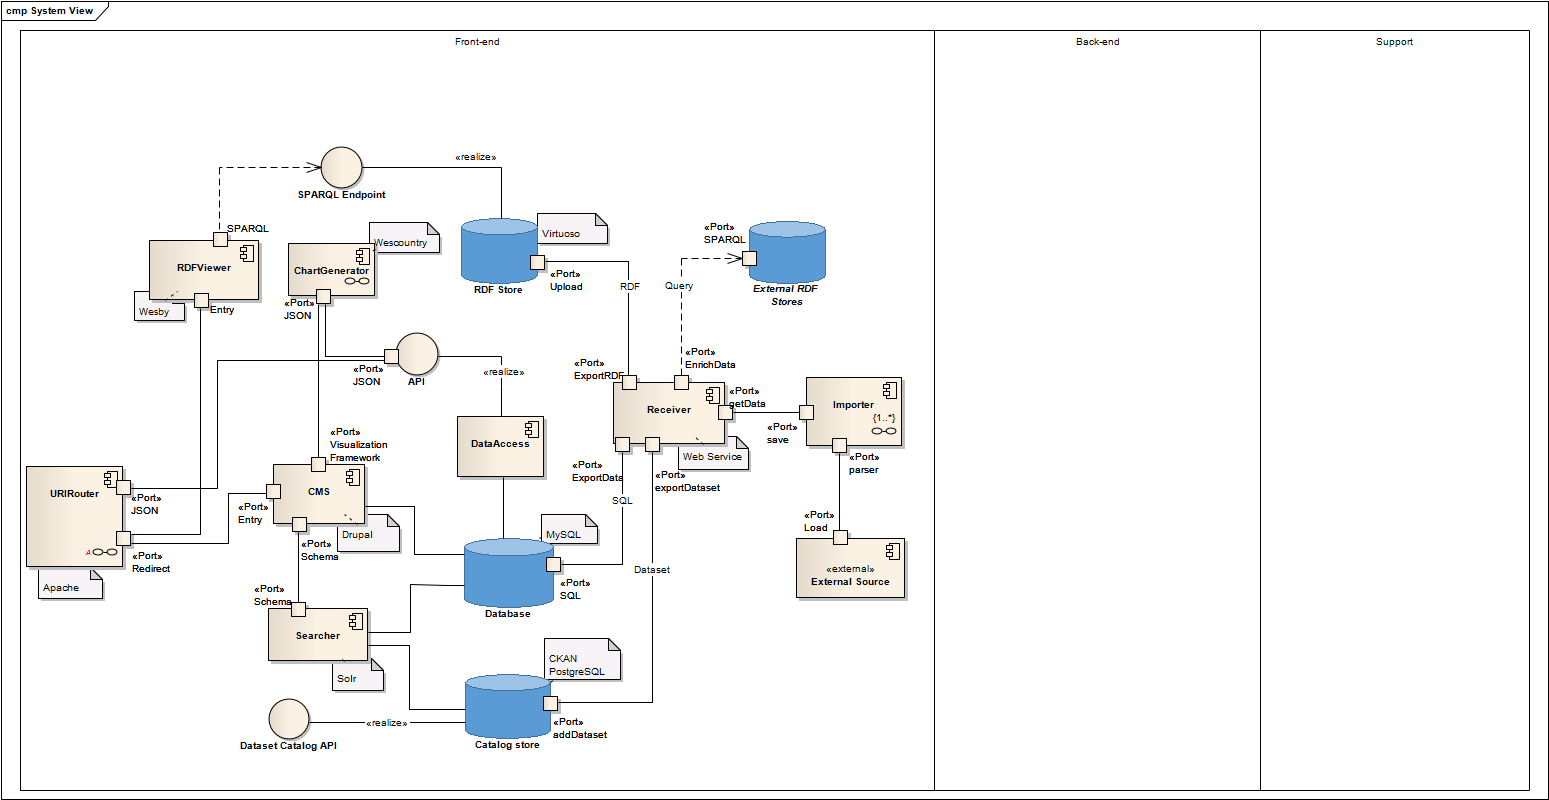
\includegraphics[height=\textwidth]{arquitectura/system_view}
		\caption{Diagrama de componentes del sistema}
		\label{fig:diagrama_componentes_sistema}
	\end{figure}
\end{landscape}


\subsubsection{Componentes}
Una vez mostrado el diagrama de componentes, se procederá a explicar el rol de cada uno de los componentes del sistema.  La descripción comenzará en los componentes más internos y terminará en los componentes más externos y cercanos al usuario del sistema.
\begin{description}
	\item[External source]  Las fuentes externas  serán fuentes de datos pertenecientes a organizaciones externas.  Estas fuentes proporcionan conjuntos de datos compuestos por indicadores y observaciones relativos a diferentes países y momentos del tiempo.  Como ya se ha mencionado en la sección ``\nameref{objetivos_proyecto}'' perteneciente al capítulo \ref{chapter01}, algunas de las fuentes externas con las que se trabajará son:
	\begin{itemize}
		\item el Banco Mundial (\textit{WorldBank})
		\item la Organización de las Naciones Unidas para la Alimentación y la Agricultura (\textit{FAO})
		\item la Organización Mundial de la Salud (\textit{WHO})
		\item el Instituto Internacional de Investigación sobre Políticas Alimentarias (\textit{IFPRI})
		\item la Organización para la Cooperación y el Desarrollo Económicos(\textit{OECD})
	\end{itemize}
	\item[Importer]  Los importadores  tendrán la tarea de transformar los conjuntos de datos provenientes de las fuentes externas a un formato común con el fin de unificar y asegurar un nivel de calidad mínimo para los datos que se insertarán en el portal.  Como se ha explicado en la sección ``\nameref{identificacion_actores}'' del capítulo \ref{chapter04}, los importadores serán los actores que interactuarán con el punto de entrada de datos, enviándole a este los conjuntos de datos ya procesados.
	\item[Receiver]  El Punto de Entrada de Datos  tendrá la misión de controlar todas las entradas de datos que se realicen hacia el portal.  Recibirá las peticiones de los importadores y almacenará los conjuntos de datos en varios servicios diferentes, concretamente: una base de datos SQL, una base de datos RDF y un catálogo de datos.  Además, el punto de entrada de datos también se encargará de enriquecer los datos antes de almacenarlos en el sistema, este enriquecimiento de datos tendrá lugar mediante la consulta de almacenamientos de RDF externos.  La arquitectura del punto de entrada de datos se verá con más detalle posteriormente en la sección ``\nameref{vista_receiver}'' de este mismo capítulo.
	\item[External RDF Stores]  Los almacenamientos (o \textit{endpoints}) de RDF externos son servicios externos que contienen información variada que se utilizará para enriquecer los datos que llegan al punto de entrada.  Un ejemplo de almacenamiento de RDF externo es \textit{DBPedia}\footnote{DBPedia contiene la información de la Wikipedia en forma de datos enlazados \url{http://dbpedia.org/About}}.
	\item[Database]  La base de datos será utilizada tanto por el gestor de contenidos y el framework de visualizaciones como por el API.  La base de datos será también uno de los lugares donde el punto de entrada almacene los catálogos de datos que llegan al portal.  El funcionamiento y esquema de la base de datos se detallará en la sección ``\nameref{diseno_modelo_datos}'' perteneciente a este mismo capítulo.
	\item[Catalog store - Dataset Catalog API]  El catálogo de datos será el encargado de almacenar los catálogos de datos que se utilizan en el portal acompañados de una serie de metadatos sobre su origen, creador, formato, etc.  Proveerá también una interfaz que permitirá a los usuarios navegar e incluso descargar en bruto los catálogos de datos almacenados en el sistema.  Como ya se explicó en la sección ``\nameref{chapter02:alternativas_seleccionadas}'' del capítulo \ref{chapter02}, el catálogo de datos seleccionado ha sido CKAN.  Al igual que la base de datos, el catálogo de datos será uno de los lugares en los que el punto de entrada almacena la información que llega al portal.
	\item[RDF Store - SPARQL endpoint]  El servidor semántico almacenará los datos en formato RDF y proveerá una punto de acceso SPARQL\footnote{SPARQL es un lenguaje de consultas capaz de manipular datos en formato RDF.  Para una mayor información al respecto véase \url{http://www.w3.org/TR/sparql11-overview/}} que podrá ser utilizado por los usuarios o por otros componentes del sistema.  Este componente será uno de los lugares donde el punto de entrada almacene los catálogos de datos que recibe.
	\item[API - DataAccess]  El API será el encargado de proporcionar una interfaz de acceso a los datos almacenados en la base de datos del sistema.  El API seguirá una arquitectura REST e incluirá un sistema de negociación de contenido con el que el cliente podrá seleccionar el formato en el que recibe los datos.  Algunos de los formatos soportados por el API serán JSON, CSV y XML.
	\item[Searcher]  El buscador será el encargado de indexar toda la información almacenada en el portal para proveer un sistema de búsqueda amigable a los usuarios.  Como se ha explicado en la sección ``\nameref{chapter02:alternativas_seleccionadas}'' del capítulo \ref{chapter02}, el buscador seleccionado ha sido Apache Solr.
	\item[CMS]  El gestor de contenidos tendrá una misión particularmente importante en el sistema final.  Será el componente que proveerá todos los subsistemas de la zona social (véase la sección ``\nameref{identificacion_subsistemas}''), además incluirá varios módulos que le permitirán comunicarse con otros componentes de la arquitectura.  Entre estos módulos destaca el módulo encargado de proporcionar el framework de soporte a las visualizaciones.  Los módulos que forman parte del gestor de contenidos podrán ser vistos con mayor detalle en la sección ``\nameref{vista_modulos_cms}'' de este mismo capítulo.
	\item[ChartGenerator]  Las visualizaciones serán las encargadas de transformar los datos en bruto almacenados en el sistema para presentarlos al usuario de una forma amigable y visual.  Par su construcción las visualizaciones utilizarán los datos devueltos por un framework que forma parte del subsistema de datos y que provee la información necesaria.  Las visualizaciones serán generadas por la librería \textit{Wescountry}
	\item[RDFViewer]  El visualizador de datos enlazados tendrá la misión de permitir a los usuarios navegar y visualizar los datos almacenados en el servidor semántico de una forma amigable y sin necesidad de realizar consultas SPARQL de forma manual.  Como se ha explicado en la sección ``\nameref{chapter02:alternativas_seleccionadas}'' del capítulo \ref{chapter02} el visualizador de datos enlazados seleccionado será \textit{Wesby}.
	\item[URIRouter]  El enrutador será el primer componente que entrará en acción del sistema ante las peticiones de los usuarios.  Su misión será redirigir la petición del usuario en función de su URL hacia el componente adecuado.  El enrutador utilizado será \textit{Apache}.
\end{description}



\subsection{Vista del punto de entrada de datos}
\label{vista_receiver}
A continuación se detallará la estructura completa del punto de entrada de datos.  Este componente del sistema también es conocido como \textit{Receiver} por ser su principal función el recibimiento y posterior almacenado de datos que provienen de fuentes externas al sistema.


\subsubsection{Diagrama de componentes}
La figura \ref{fig:diagrama_componentes_receiver} muestra el diagrama de todos los componentes que conforman el punto de entrada de datos.

El punto de entrada de datos está construido como una aplicación web que escucha peticiones del exterior y las procesa para almacenar los datos que recibe en diferentes puntos de almacenamiento.
\begin{landscape}
	\begin{figure}[ht]
		\centering
		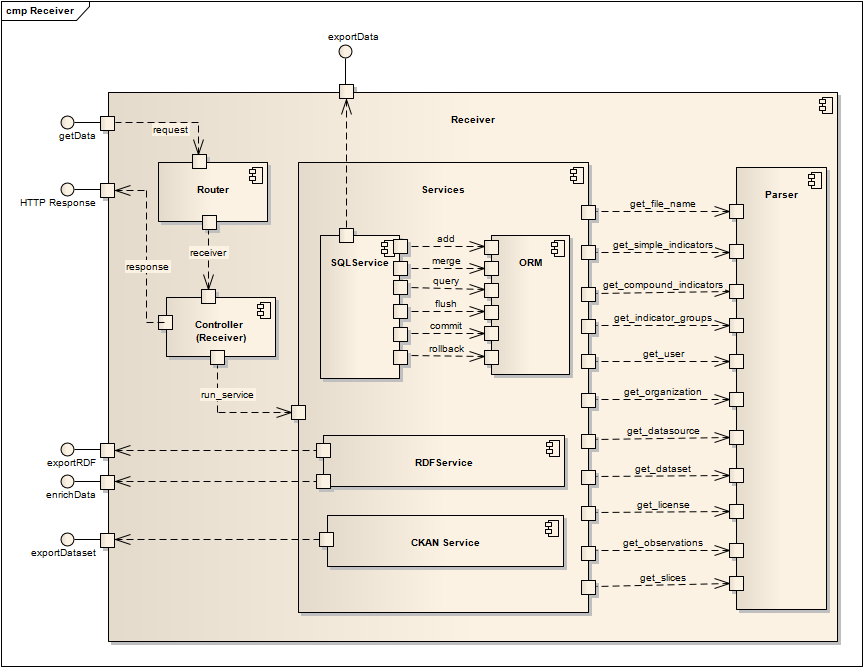
\includegraphics[height=\textwidth]{arquitectura/receiver_view}
		\caption{Diagrama de componentes del punto de entrada de datos}
		\label{fig:diagrama_componentes_receiver}
	\end{figure}
\end{landscape}


\subsubsection{Descripción de los componentes}
Tras haber mostrado el diagrama de los componentes que forman parte del punto de entrada de datos es el momento de explicar el papel que juega cada uno de ellos.

\begin{description}
	\item[Router]  El enrutador se encarga de dirigir las peticiones HTTP que provienen del exterior hacia el controlador.  También es el encargado de responder a las peticiones que no se correspondan con ningún controlador, o que no utilicen un verbo adecuado.
	\item[Controller (Receiver)]  El controlador se encarga de las peticiones de inserción de datos.  Su misión es comprobar si la petición que recibe tiene una forma adecuada y llamar a los distintos servicios para que procesen los datos.
	\item[Parser]  El parser es el encargado de transformar los datos provenientes de las peticiones externas a un modelo de datos que será utilizado por los servicios para realizar los diferentes procesados.  El modelo de datos será visto con más detalle en la sección ``\nameref{diseno_modelo_datos}'' de este mismo capítulo.
	\item[SQLService]  El servicio de SQL se encarga de procesar los datos que llegan al punto de entrada y generar las consultas necesarias para almacenarlos en una base de datos relacional.  Este servicio delega la generación de consultas SQL al ORM.
	\item[ORM]  El Mapeador Objeto-Relacional actúa como una capa de abstracción sobre la base de datos y permite al desarrollador trabajar con objetos sin necesidad de ocuparse de su transformación al modelo relacional.
	\item[RDFService]  El servicio de RDF se encarga de procesar los datos que llegan al punto de entrada y generar los grafos RDF que serán almacenados en el servidor semántico.
	\item[CKANService]  El servicio de CKAN se encarga de procesar los datos que llegan al punto de entrada y generar los metadatos que se almacenan en el catálogo de datos.
\end{description}


\subsubsection{Relacion entre los componentes}
Las peticiones provenientes de los importadores llegan al enrutador.  El enrutador redirige las peticiones que utilicen un verbo adecuado (POST) hacia el controlador, quien comprueba si la petición cuenta con todos los parámetros necesarios.

Si la petición cuenta con los parámetros adecuados, el controlador llama a cada uno de los servicios para que realicen su trabajo.  Los distintos servicios utilizarán a su vez el parser para convertir la información que proviene de la petición a un modelo de datos con el que ellos pueden trabajar.


\subsubsection{Interfaces y puertos}
A continuación se detallarán las interfaces y puertos de los componentes que forman parte del punto de entrada de datos. 

\paragraph{Receiver} \hfill \\
La tabla \ref{interfaces_receiver_receiver} muestra el detalle de las interfaces del \textit{Receiver}.
\begin{longtable}[c]{|p{25mm}|p{20mm}|p{30mm}|p{60mm}|}
 \caption{Vista del punto de entrada de datos - interfaces del \textit{Receiver}.\label{interfaces_receiver_receiver}}\\

 %Cabecera en la primera pagina
 \hline
 	Interfaz & Tipo & Tecnología & Propiedades\\
 \hline
 \hline
 \endfirsthead
 %Cabecera en el resto de páginas
 \hline
 \multicolumn{4}{|c|}{Continuación de la tabla \ref{interfaces_receiver_receiver}}\\
 \hline
 	Interfaz & Tipo & Tecnología & Propiedades\\
 \hline
 \hline
 \endhead
 %Tabla
 \hline
 \endfoot
 
	\textbf{HTTP Request} & Proveída & Servicio web REST & Recibe las peticiones procedentes del exterior \\
	\hline
		
	\textbf{HTTP Response} & Proveída & Servicio web REST & Responde a las peticiones HTTP recibidas \\
	\hline
	
	\textbf{exportRDF} & Requerida & API del servidor semántico & Exporta en formato RDF los datos recibidos de la petición \\
	\hline
	
	\textbf{exportData} & Requerida & Consultas a base de datos & Exporta en formato SQL los datos recibidos de la petición \\
	\hline
	
	\textbf{exportDataset} & Requerida & API del catálogo de datos & Exporta el catálogo de datos recibido de la petición junto con sus metadatos \\
	\hline
	
	\textbf{enrichData} & Requerida & Consultas SPARQL & Enriquece los datos mediante consultas SPARQL a servidores semánticos externos \\
\hline
\hline

 \end{longtable}
 
 
 \paragraph{Router} \hfill \\
 La tabla \ref{interfaces_receiver_router} muestra el detalle de las interfaces del \textit{Router}.
 \begin{longtable}[c]{|p{25mm}|p{20mm}|p{30mm}|p{60mm}|}
  \caption{Vista del punto de entrada de datos - interfaces del \textit{Router}.\label{interfaces_receiver_router}}\\
 
  %Cabecera en la primera pagina
  \hline
  	Interfaz & Tipo & Tecnología & Propiedades\\
  \hline
  \hline
  \endfirsthead
  %Cabecera en el resto de páginas
  \hline
  \multicolumn{4}{|c|}{Continuación de la tabla \ref{interfaces_receiver_router}}\\
  \hline
  	Interfaz & Tipo & Tecnología & Propiedades\\
  \hline
  \hline
  \endhead
  %Tabla
  \hline
  \endfoot
  
 	\textbf{HTTP Request} & Puerto de entrada & Servicio web REST & Recibe las peticiones procedentes del exterior \\
 	\hline
 	
 	\textbf{receiver} & Puerto de salida & Llamada a método & Pasa la petición al controlador correspondiente tras haber comprobado que utiliza el verbo adecuado \\
 \hline
 \hline
 
  \end{longtable}
  
\paragraph{Controller} \hfill \\
La tabla \ref{interfaces_receiver_controller} muestra el detalle de las interfaces del \textit{Controller}.

\begin{longtable}[c]{|p{25mm}|p{20mm}|p{30mm}|p{60mm}|}
 \caption{Vista del punto de entrada de datos - interfaces del textit{Controller}.\label{interfaces_receiver_controller}}\\
   %Cabecera en la primera pagina
 \hline
 	Interfaz & Tipo & Tecnología & Propiedades\\
 \hline
 \hline
 \endfirsthead
 %Cabecera en el resto de páginas
 \hline
 \multicolumn{4}{|c|}{Continuación de la tabla \ref{interfaces_receiver_controller}}\\
 \hline
 	Interfaz & Tipo & Tecnología & Propiedades\\
 \hline
 \hline
 \endhead
 %Tabla
 \hline
 \endfoot
 	
 	\textbf{receiver} & Puerto de entrada & Llamada a método & Recibe la petición procedente el enrutador y comprueba si incluye todos los parámetros necesarios \\
 	\hline
 	
 	\textbf{run service} & Puerto de salida & Llamada a método & Ejecuta la funcionalidad de un servicio \\
 	\hline
 	
 	\textbf{response} & Puerto de salida & Servicio web REST & Envía una respuesta con un código de error HTTP adecuado en función del éxito o no en el procesamiento de la petición. \\
\hline
\hline
 
\end{longtable}


\paragraph{Interfaces comunes a todos los servicios} \hfill \\
La tabla \ref{interfaces_receiver_services} muestra el detalle de las interfaces comunes a todos los servicios.

\begin{longtable}[c]{|p{25mm}|p{20mm}|p{30mm}|p{60mm}|}
 \caption{Vista del punto de entrada de datos - interfaces comunes a todos los servicios.\label{interfaces_receiver_services}}\\
 %Cabecera en la primera pagina
 \hline
 	Interfaz & Tipo & Tecnología & Propiedades\\
 \hline
 \hline
 \endfirsthead
 %Cabecera en el resto de páginas
 \hline
 \multicolumn{4}{|c|}{Continuación de la tabla \ref{interfaces_receiver_services}}\\
 \hline
 	Interfaz & Tipo & Tecnología & Propiedades\\
 \hline
 \hline
 \endhead
 %Tabla
 \hline
 \endfoot
 
 	\textbf{run service} & Puerto de entrada & Llamada a método & Comienza la ejecución del servicio \\
 	\hline
 	
 	\textbf{get file name} & Puerto de salida & Llamada a método & Obtiene el nombre del fichero que contiene los datos en bruto \\
 	\hline
 	
 	\textbf{get simple indicators} & Puerto de salida & Llamada a método & Obtiene una lista de los indicadores simples obtenidos del fichero de datos \\
 	\hline
 	
 	\textbf{get compound indicators} & Puerto de salida & Llamada a método & Obtiene una lista de los indicadores compuestos obtenidos del fichero de datos \\
 	\hline
 	
  	\textbf{get user} & Puerto de salida & Llamada a método & Obtiene los del usuario que realiza la petición de inserción de datos \\
  	\hline
  	
  	\textbf{get organization} & Puerto de salida & Llamada a método & Obtiene la información sobre la organización que proporciona el fichero de datos \\
  	\hline
  	
   	\textbf{get datasource} & Puerto de salida & Llamada a método & Obtiene la información sobre la fuente de datos de la que procede el fichero de datos \\
   	\hline
   	
   	\textbf{get dataset} & Puerto de salida & Llamada a método & Obtiene la información sobre el propio fichero de datos\\
   	\hline
   	
   	\textbf{get license} & Puerto de salida & Llamada a método & Obtiene la información sobre la licencia bajo la que se publica el fichero de datos \\
   	\hline
   	
   	\textbf{get observations} & Puerto de salida & Llamada a método & Obtiene la lista de observaciones procedentes del fichero de datos \\
   	\hline
   	
   	\textbf{get slices} & Puerto de salida & Llamada a método & Obtiene la lista con las \textit{slices}\footnote{Para más información sobre las \textit{slices} véase la sección ``\nameref{concept:rdf_data_cube}'' perteneciente al capítulo \ref{chapter03}} procedentes del fichero de datos. \\
   	\hline
\hline
\hline
 
\end{longtable}


\paragraph{Interfaces del \textit{Parser}} \hfill \\
La tabla \ref{interfaces_receiver_parser} muestra el detalle de las interfaces pertenecientes al \textit{Parser}.

\begin{longtable}[c]{|p{25mm}|p{20mm}|p{30mm}|p{60mm}|}
 \caption{Vista del punto de entrada de datos - interfaces pertenecientes al \textit{Parser}.\label{interfaces_receiver_parser}}\\
 %Cabecera en la primera pagina
 \hline
 	Interfaz & Tipo & Tecnología & Propiedades\\
 \hline
 \hline
 \endfirsthead
 %Cabecera en el resto de páginas
 \hline
 \multicolumn{4}{|c|}{Continuación de la tabla \ref{interfaces_receiver_parser}}\\
 \hline
 	Interfaz & Tipo & Tecnología & Propiedades\\
 \hline
 \hline
 \endhead
 %Tabla
 \hline
 \endfoot
 	
 	\textbf{get file name} & Puerto de entrada & Llamada a método & Devuelve el nombre del fichero que contiene los datos en bruto \\
 	\hline
 	
 	\textbf{get simple indicators} & Puerto de entrada & Llamada a método & Devuelve una lista de los indicadores simples obtenidos del fichero de datos \\
 	\hline
 	
 	\textbf{get compound indicators} & Puerto de entrada & Llamada a método & Devuelve una lista de los indicadores compuestos obtenidos del fichero de datos \\
 	\hline
 	
  	\textbf{get user} & Puerto de salida & Llamada a entrada & Devuelve los del usuario que realiza la petición de inserción de datos \\
  	\hline
  	
  	\textbf{get organization} & Puerto de entrada & Llamada a método & Devuelve la información sobre la organización que proporciona el fichero de datos \\
  	\hline
  	
   	\textbf{get datasource} & Puerto de entrada & Llamada a método & Devuelve la información sobre la fuente de datos de la que procede el fichero de datos \\
   	\hline
   	
   	\textbf{get dataset} & Puerto de entrada & Llamada a método & Devuelve la información sobre el propio fichero de datos\\
   	\hline
   	
   	\textbf{get license} & Puerto de entrada & Llamada a método & Devuelve la información sobre la licencia bajo la que se publica el fichero de datos \\
   	\hline
   	
   	\textbf{get observations} & Puerto de entrada & Llamada a método & Devuelve la lista de observaciones procedentes del fichero de datos \\
   	\hline
   	
   	\textbf{get slices} & Puerto de entrada & Llamada a método & Devuelve la lista con las \textit{slices} procedentes del fichero de datos. \\
   	\hline
\hline
\hline
 
\end{longtable}


\paragraph{SQLService} \hfill \\
La tabla \ref{interfaces_receiver_sqlservice} muestra el detalle de las interfaces del \textit{servicio de SQL} que no han sido incluidas anteriormente en la tabla \ref{interfaces_receiver_services}.  

\begin{longtable}[c]{|p{25mm}|p{20mm}|p{30mm}|p{60mm}|}
	\caption{Vista del punto de entrada de datos - interfaces del \textit{servicio de SQL}.\label{interfaces_receiver_sqlservice}}\\
	%Cabecera en la primera pagina
		\hline
			Interfaz & Tipo & Tecnología & Propiedades\\
		\hline
		\hline
	\endfirsthead
	%Cabecera en el resto de páginas
		\hline
		\multicolumn{4}{|c|}{Continuación de la tabla \ref{interfaces_receiver_sqlservice}}\\
		\hline
			Interfaz & Tipo & Tecnología & Propiedades\\
		\hline
		\hline
	\endhead
	%Tabla
	\hline
	\endfoot
		\textbf{exportData} & Requerida & Consultas a base de datos & Exporta en formato SQL los datos recibidos de la petición \\
		\hline
		\textbf{add} & Puerto de salida & Llamada a método & Almacena los datos de un objeto del modelo en la base de datos \\
		\hline
		\textbf{merge} & Puerto de salida & Llamada a método & Actualiza los datos de un objeto del modelo en la base de datos \\
		\hline
		\textbf{query} & Puerto de salida & Llamada a método & Realiza una consulta a la base de datos y devuelve los resultados\\
		\hline
		\textbf{flush} & Puerto de salida & Llamada a método & Vuelca los cambios realizados en memoria a la base de datos \\
		\hline
		\textbf{commit} & Puerto de salida & Llamada a método & Cierra una transacción con la base de datos \\
		\hline
		\textbf{rollback} & Puerto de salida & Llamada a método & Deshace los cambios de la transacción en curso\\
		\hline
	\hline
	\hline
\end{longtable}


\paragraph{ORM} \hfill \\
La tabla \ref{interfaces_receiver_orm} muestra el detalle de las interfaces del \textit{ORM}.  

\begin{longtable}[c]{|p{25mm}|p{20mm}|p{30mm}|p{60mm}|}
	\caption{Vista del punto de entrada de datos - interfaces del \textit{ORM}.\label{interfaces_receiver_orm}}\\
	%Cabecera en la primera pagina
		\hline
			Interfaz & Tipo & Tecnología & Propiedades\\
		\hline
		\hline
	\endfirsthead
	%Cabecera en el resto de páginas
		\hline
		\multicolumn{4}{|c|}{Continuación de la tabla \ref{interfaces_receiver_orm}}\\
		\hline
			Interfaz & Tipo & Tecnología & Propiedades\\
		\hline
		\hline
	\endhead
	%Tabla
	\hline
	\endfoot
		\textbf{add} & Puerto de entrada & Llamada a método & Almacena los datos de un objeto del modelo en la base de datos \\
		\hline
		\textbf{merge} & Puerto de entrada & Llamada a método & Actualiza los datos de un objeto del modelo en la base de datos \\
		\hline
		\textbf{query} & Puerto de entrada & Llamada a método & Realiza una consulta a la base de datos y devuelve los resultados\\
		\hline
		\textbf{flush} & Puerto de entrada & Llamada a método & Vuelca los cambios realizados en memoria a la base de datos \\
		\hline
		\textbf{commit} & Puerto de entrada & Llamada a método & Cierra una transacción con la base de datos \\
		\hline
		\textbf{rollback} & Puerto de entrada & Llamada a método & Deshace los cambios de la transacción en curso\\
		\hline
	\hline
	\hline
\end{longtable}


\paragraph{RDFService} \hfill \\
La tabla \ref{interfaces_receiver_rdfservice} muestra el detalle de las interfaces del \textit{servicio de RDF} que no han sido incluidas anteriormente en la tabla \ref{interfaces_receiver_services}.  

\begin{longtable}[c]{|p{25mm}|p{20mm}|p{30mm}|p{60mm}|}
	\caption{Vista del punto de entrada de datos - interfaces del \textit{servicio de RDF}.\label{interfaces_receiver_rdfservice}}\\
	%Cabecera en la primera pagina
		\hline
			Interfaz & Tipo & Tecnología & Propiedades\\
		\hline
		\hline
	\endfirsthead
	%Cabecera en el resto de páginas
		\hline
		\multicolumn{4}{|c|}{Continuación de la tabla \ref{interfaces_receiver_rdfservice}}\\
		\hline
			Interfaz & Tipo & Tecnología & Propiedades\\
		\hline
		\hline
	\endhead
	%Tabla
	\hline
	\endfoot
		\textbf{exportRDF} & Requerida & API del servidor semántico & Exporta en formato RDF los datos recibidos de la petición \\
		\hline
		\textbf{enrichData} & Requerida & Consultas SPARQL & Enriquece los datos mediante consultas SPARQL a servidores semánticos externos \\
	\hline
	\hline
\end{longtable}


\paragraph{CKANService} \hfill \\
La tabla \ref{interfaces_receiver_ckanservice} muestra el detalle de las interfaces del \textit{servicio de CKAN} que no han sido incluidas anteriormente en la tabla \ref{interfaces_receiver_services}.  

\begin{longtable}[c]{|p{25mm}|p{20mm}|p{30mm}|p{60mm}|}
	\caption{Vista del punto de entrada de datos - interfaces del \textit{servicio de CKAN}.\label{interfaces_receiver_ckanservice}}\\
	%Cabecera en la primera pagina
		\hline
			Interfaz & Tipo & Tecnología & Propiedades\\
		\hline
		\hline
	\endfirsthead
	%Cabecera en el resto de páginas
		\hline
		\multicolumn{4}{|c|}{Continuación de la tabla \ref{interfaces_receiver_ckanservice}}\\
		\hline
			Interfaz & Tipo & Tecnología & Propiedades\\
		\hline
		\hline
	\endhead
	%Tabla
	\hline
	\endfoot
		\textbf{exportDataset} & Requerida & API del catálogo de datos & Exporta el catálogo de datos recibido de la petición junto con sus metadatos \\
	\hline
	\hline
\end{longtable}


\subsection{Vista de los módulos del gestor de contenidos}
\label{vista_modulos_cms}
A continuación se detallará la estructura completa del gestor de contenidos.  Como se ha explicado en la sección ``\nameref{chapter02:alternativas_seleccionadas}'' perteneciente al capítulo \ref{chapter02}, el gestor de contenidos seleccionado ha sido Drupal.


\subsubsection{Diagrama de componentes}
La figura \ref{fig:diagrama_componentes_cms} muestra el diagrama de los componentes que forman parte del gestor de contenidos.
\begin{landscape}
	\begin{figure}[ht]
		\centering
		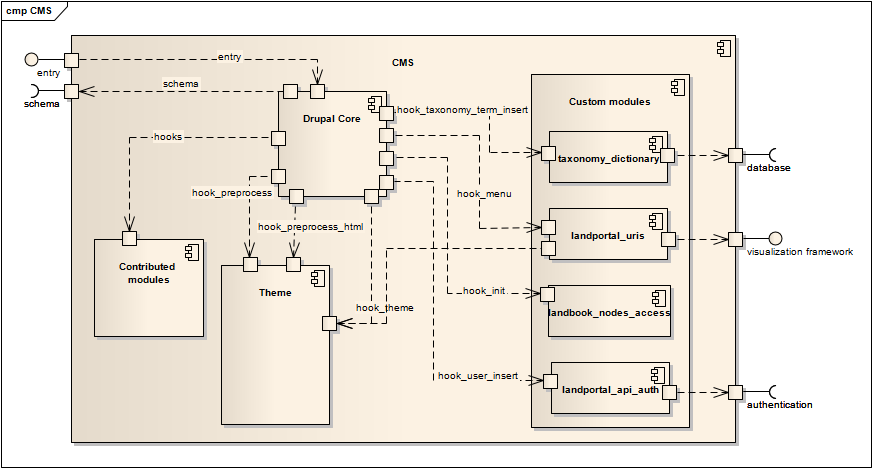
\includegraphics[height=\textwidth]{arquitectura/cms_view}
		\caption{Diagrama de componentes del gestor de contenidos}
		\label{fig:diagrama_componentes_cms}
	\end{figure}
\end{landscape}


\subsubsection{Descripción de los componentes}
Se describirán ahora los distintos componentes que forman parte del gestor de contenidos.
\begin{description}
	\item[Drupal Core]  El núcleo de Drupal implementa la funcionalidad principal del gestor de contenidos.  Es el encargado de procesar y responder a las peticiones, además de coordinar el funcionamiento de los diferentes módulos y temas visuales.
	\item[Contributed modules]  Los módulos contribuidos son módulos realizados por terceros y que han sido públicamente incluidos en el repositorio de módulos de Drupal.  Éstos módulos amplían la funcionalidad existente en el núcleo de Drupal\footnote{Actualmente existen unos 15.000 módulos que forman parte del repositorio.  Dichos módulos pueden verse en \url{https://www.drupal.org/project/project_module}}.
	\item[Custom modules]  Los módulos propios han sido especialmente creados para éste proyecto y realizan alguna funcionalidad que no forma parte del núcleo de Drupal ni de ningún módulo contribuido.  Se han desarrollado cuatro módulos propios:
		\begin{itemize}
			\item \textit{taxonomy\_dictionary}  Permite relacionar los datos existentes en la base de datos con los términos de las taxonomías existentes en Drupal.
			\item \textit{landportal\_uris}  Implementa un sistema similar al MVC para facilitar la creación de vistas.  También incluye el framework que provee de datos a las visualizaciones.  Éste módulo se verá con más detalle posteriormente en la sección ``\nameref{vista_landportal_uris}'' de éste mismo capítulo.
			\item \textit{landbook\_nodes\_access}  Permite redirigir a las vistas adecuadas cuando se visite alguno de los nodos de la sección de datos.
			\item \textit{landportal\_api\_auth}  Genera y almacena las claves de autenticación del el API para los nuevos usuarios que se creen en el sistema.
		\end{itemize}
	\item[Theme]  El tema implementa la interfaz de las diferentes vistas que forman parte del gestor de contenidos.
\end{description}


\subsubsection{Relación entre los componentes}
Las peticiones entrantes son procesadas por el núcleo de Drupal.  En cada petición el núcleo de Drupal invoca los módulos que estén suscritos a los \textit{hooks} adecuados para que realicen su funcionalidad\footnote{El módulo ``\textit{landportal\_uris}'' será detallado posteriormente en la sección ``\nameref{vista_landportal_uris}'' de éste mismo capítulo.  El resto de módulos propios cuentan simplemente con un único fichero que implementa el \textit{hook} correspondiente por lo que, dada su sencillez, sus vistas se omitirán}:
\begin{itemize}
	\item Cuando se crea un nuevo término en la taxonomía se invoca al módulo \textit{taxonomy\_dictionary} para que lo enlace con el término correspondiente en la base de datos.
	\item Cuando se realiza una petición que no va dirigida a mostrar la vista de administración se invoca al módulo \textit{landportal\_uris} para que provea los datos con los que se renderizarán posteriormente las vistas del tema.  Éste procedimiento será posteriormente detallado en la sección INCLUIR SECCION.
	\item Cuando se accede a alguno de los nodos pertenecientes a la zona de datos se invoca al módulo \textit{landbook\_nodes\_access} para que realice la redirección hacia la vista adecuada.
	\item Cuando se crea un nuevo usuario en el portal se invoca al módulo \textit{landportal\_api\_auth} para que cree y almacene sus claves de acceso al API.
\end{itemize}
Por último, el núcleo de Drupal invoca al tema para que renderice las vistas que serán mostradas al usuario que realiza la petición.


\subsubsection{Interfaces y puertos}
A continuación se detallarán las interfaces y puertos de los componentes que forman parte del gestor de contenidos. 

\paragraph{CMS} \hfill \\
La tabla \ref{interfaces_cms_cms} muestra el detalle de las interfaces del \textit{CMS}.

\begin{longtable}[c]{|p{25mm}|p{20mm}|p{30mm}|p{60mm}|}
 \caption{Vista del gestor de contenidos - interfaces del \textit{CMS}.\label{interfaces_cms_cms}}\\

 %Cabecera en la primera pagina
 \hline
 	Interfaz & Tipo & Tecnología & Propiedades\\
 \hline
 \hline
 \endfirsthead
 %Cabecera en el resto de páginas
 \hline
 \multicolumn{4}{|c|}{Continuación de la tabla \ref{interfaces_receiver_receiver}}\\
 \hline
 	Interfaz & Tipo & Tecnología & Propiedades\\
 \hline
 \hline
 \endhead
 %Tabla
 \hline
 \endfoot
 
	\textbf{entry} & Proveída & Petición HTTP & Recibe las peticiones procedentes del exterior \\
	\hline
		
	\textbf{schema} & Requerida & API del motor de búsqueda & Envía los datos del gestor de contenidos al motor de búsqueda para su indexación\footnote{ Como se ha explicado en la sección ``\nameref{chapter02:alternativas_seleccionadas}'' perteneciente al capítulo \ref{chapter02}, el motor de búsqueda seleccionado ha sido \textit{Apache Solr}} \\
	\hline
	
	\textbf{database} & Requerida & Conexión a base de datos & Accede a la base de datos donde se almacena la información perteneciente al subsistema de datos \\
	\hline
	
	\textbf{visualization framework} & Proveída & API Web & Provee datos con los que posteriormente crear las visualizaciones\footnote{Los elementos de éste framework podrán ser vistos con mayor detalle posteriormente en la sección ``\nameref{vista_landportal_uris}'' perteneciente a éste mismo capítulo} \\
	\hline
	
	\textbf{authentication} & Proveída & API REST & Genera claves de autenticación en el API para los usuarios del portal \\
\hline
\hline

 \end{longtable}


\paragraph{Drupal Core} \hfill \\
La tabla \ref{interfaces_cms_drupalcore} muestra el detalle de las interfaces del \textit{núcleo de Drupal}.  

\begin{longtable}[c]{|p{25mm}|p{20mm}|p{30mm}|p{60mm}|}
	\caption{Vista del gestor de contenidos - interfaces del \textit{núcleo de Drupal}.\label{interfaces_cms_drupalcore}}\\
	%Cabecera en la primera pagina
		\hline
			Interfaz & Tipo & Tecnología & Propiedades\\
		\hline
		\hline
	\endfirsthead
	%Cabecera en el resto de páginas
		\hline
		\multicolumn{4}{|c|}{Continuación de la tabla \ref{interfaces_cms_drupalcore}}\\
		\hline
			Interfaz & Tipo & Tecnología & Propiedades\\
		\hline
		\hline
	\endhead
	%Tabla
	\hline
	\endfoot
		\textbf{entry} & Puerto de entrada & Petición HTTP & Recibe las peticiones procedentes del exterior \\
		\hline
		
		\textbf{schema} & Puerto de salida & API del motor de búsqueda & Envía los datos del gestor de contenidos al motor de búsqueda para su indexación \\
		\hline
		
		\textbf{hooks} & Puerto de salida & Llamada a método & Invoca a los módulos que estén suscritos al \textit{hook} correspondiente \\
		\hline
		
		\textbf{hook preprocess} & Puerto de salida & Llamada a método & Indica al tema que preprocese las variables que sean necesarias para las vistas \\
		\hline
		
		\textbf{hook preprocess html} & Puerto de salida & Llamada a método & Indica al tema que preprocese las variables que sean necesarias para la plantilla HTML \\
		\hline
		
		\textbf{hook theme} & Puerto de salida & Llamada a método & Indica al tema que renderice una determinada plantilla para una vista \\
		\hline
		
		\textbf{hook taxonomy term insert} & Puerto de salida & Llamada a método & Indica a un módulo que se ha creado un nuevo término en la taxonomía para que éste realice su funcionalidad \\
		\hline
		
		\textbf{hook menu} & Puerto de salida & Llamada a método & Permite a un módulo registrar rutas para definir cómo son atendidas las peticiones HTTP \\
		\hline
		
		\textbf{hook init} & Puerto de salida & Llamada a método & Indica a un módulo que acaba de tener lugar una petición por parte de un usuario \\
		\hline
		
		\textbf{hook user insert} & Puerto de salida & Llamada a método & Indica a un módulo que acaba de producirse el registro de un nuevo usuario \\
	\hline
	\hline
\end{longtable}


\paragraph{Contributed modules} \hfill \\
La tabla \ref{interfaces_cms_modules} muestra el detalle de las interfaces de los \textit{módulos contribuidos}.  

\begin{longtable}[c]{|p{25mm}|p{20mm}|p{30mm}|p{60mm}|}
	\caption{Vista del gestor de contenidos - interfaces de los \textit{módulos contribuidos}.\label{interfaces_cms_modules}}\\
	%Cabecera en la primera pagina
		\hline
			Interfaz & Tipo & Tecnología & Propiedades\\
		\hline
		\hline
	\endfirsthead
	%Cabecera en el resto de páginas
		\hline
		\multicolumn{4}{|c|}{Continuación de la tabla \ref{interfaces_cms_modules}}\\
		\hline
			Interfaz & Tipo & Tecnología & Propiedades\\
		\hline
		\hline
	\endhead
	%Tabla
	\hline
	\endfoot
		\textbf{hooks} & Puerto de entrada & Llamada a método & Invocados por el núcleo de Drupal cuando tienen lugar ciertos eventos en el sistema \\
	\hline
	\hline
\end{longtable}


\paragraph{Theme} \hfill \\
La tabla \ref{interfaces_cms_theme} muestra el detalle de las interfaces del \textit{tema}.  

\begin{longtable}[c]{|p{25mm}|p{20mm}|p{30mm}|p{60mm}|}
	\caption{Vista del gestor de contenidos - interfaces del \textit{tema}.\label{interfaces_cms_theme}}\\
	%Cabecera en la primera pagina
		\hline
			Interfaz & Tipo & Tecnología & Propiedades\\
		\hline
		\hline
	\endfirsthead
	%Cabecera en el resto de páginas
		\hline
		\multicolumn{4}{|c|}{Continuación de la tabla \ref{interfaces_cms_theme}}\\
		\hline
			Interfaz & Tipo & Tecnología & Propiedades\\
		\hline
		\hline
	\endhead
	%Tabla
	\hline
	\endfoot
		\textbf{hook preprocess} & Puerto de entrada & Llamada a método & Preprocesa las variables que sean necesarias para la posterior renderización de las vistas \\
		\hline
			
		\textbf{hook preprocess html} & Puerto de entrada & Llamada a método & Preprocesa las variables necesarias para renderizar la plantilla HTML \\
		\hline
			
		\textbf{hook theme} & Puerto de entrada & Llamada a método & Renderiza la plantilla de una determinada vista \\
	\hline
	\hline
\end{longtable}


\paragraph{Taxonomy dictionary} \hfill \\
La tabla \ref{interfaces_cms_taxonomy_dictionary} muestra el detalle de las interfaces del módulo ``\textit{Taxonomy dictionary}''.  

\begin{longtable}[c]{|p{25mm}|p{20mm}|p{30mm}|p{60mm}|}
	\caption{Vista del gestor de contenidos - interfaces del módulo \textit{Taxonomy dictionary}. \label{interfaces_cms_taxonomy_dictionary}}\\
	%Cabecera en la primera pagina
		\hline
			Interfaz & Tipo & Tecnología & Propiedades\\
		\hline
		\hline
	\endfirsthead
	%Cabecera en el resto de páginas
		\hline
		\multicolumn{4}{|c|}{Continuación de la tabla \ref{interfaces_cms_taxonomy_dictionary}}\\
		\hline
			Interfaz & Tipo & Tecnología & Propiedades\\
		\hline
		\hline
	\endhead
	%Tabla
	\hline
	\endfoot
		\textbf{hook taxonomy term insert} & Puerto de entrada & Llamada a método & Recibe la información de un nuevo término que se ha creado en la taxonomía \\
		\hline
		\textbf{database} & Puerto de salida & Conexión a base de datos & Almacena la información del término insertado en la taxonomía en la entrada correspondiente de la base de datos \\
	\hline
	\hline
\end{longtable}


\paragraph{LandPortal URIs} \hfill \\
La tabla \ref{interfaces_cms_landportal_uris} muestra el detalle de las interfaces del módulo ``\textit{LandPortal URIs}''.  

\begin{longtable}[c]{|p{25mm}|p{20mm}|p{30mm}|p{60mm}|}
	\caption{Vista del gestor de contenidos - interfaces del módulo \textit{LandPortal URIs}. \label{interfaces_cms_landportal_uris}}\\
	%Cabecera en la primera pagina
		\hline
			Interfaz & Tipo & Tecnología & Propiedades\\
		\hline
		\hline
	\endfirsthead
	%Cabecera en el resto de páginas
		\hline
		\multicolumn{4}{|c|}{Continuación de la tabla \ref{interfaces_cms_landportal_uris}}\\
		\hline
			Interfaz & Tipo & Tecnología & Propiedades\\
		\hline
		\hline
	\endhead
	%Tabla
	\hline
	\endfoot
		\textbf{hook menu} & Puerto de entrada & Llamada a método & El gestor de contenidos está definiendo las rutas que tendrán las vistas del portal \\
		\hline
		\textbf{hook theme} & Puerto de salida & Llamada a método & Indica al tema que renderice una determinada plantilla para una vista \\
		\hline
		\textbf{visualization framework} & Puerto de salida & API Web & Provee datos con los que posteriormente crear las visualizaciones \\
		\hline
		\textbf{database} & Puerto de salida & Conexión a base de datos & Obtiene información de la base de datos \\
	\hline
	\hline
\end{longtable}


\paragraph{LandbBook nodes access} \hfill \\
La tabla \ref{interfaces_cms_landbook_nodes_access} muestra el detalle de las interfaces del módulo ``\textit{LandbBook nodes access}''.  

\begin{longtable}[c]{|p{25mm}|p{20mm}|p{30mm}|p{60mm}|}
	\caption{Vista del gestor de contenidos - interfaces del módulo \textit{LandbBook nodes access}. \label{interfaces_cms_landbook_nodes_access}}\\
	%Cabecera en la primera pagina
		\hline
			Interfaz & Tipo & Tecnología & Propiedades\\
		\hline
		\hline
	\endfirsthead
	%Cabecera en el resto de páginas
		\hline
		\multicolumn{4}{|c|}{Continuación de la tabla \ref{interfaces_cms_landbook_nodes_access}}\\
		\hline
			Interfaz & Tipo & Tecnología & Propiedades\\
		\hline
		\hline
	\endhead
	%Tabla
	\hline
	\endfoot
		\textbf{hook init} & Puerto de entrada & Llamada a método & Invocada por el núcleo del gestor de contenidos cuando acaba de tener lugar una petición por parte de un usuario \\
	\hline
	\hline
\end{longtable}


\paragraph{Landportal API auth} \hfill \\
La tabla \ref{interfaces_cms_landportal_api_auth} muestra el detalle de las interfaces del módulo ``\textit{LandPortal API auth}''.  

\begin{longtable}[c]{|p{25mm}|p{20mm}|p{30mm}|p{60mm}|}
	\caption{Vista del gestor de contenidos - interfaces del módulo \textit{LandPortal API auth}. \label{interfaces_cms_landportal_api_auth}}\\
	%Cabecera en la primera pagina
		\hline
			Interfaz & Tipo & Tecnología & Propiedades\\
		\hline
		\hline
	\endfirsthead
	%Cabecera en el resto de páginas
		\hline
		\multicolumn{4}{|c|}{Continuación de la tabla \ref{interfaces_cms_landportal_api_auth}}\\
		\hline
			Interfaz & Tipo & Tecnología & Propiedades\\
		\hline
		\hline
	\endhead
	%Tabla
	\hline
	\endfoot
		\textbf{hook user insert} & Puerto de entrada & Llamada a método & Invocado por el núcleo del gestor de contenidos cuando se realiza el registro de un nuevo usuario \\
		\hline
		\textbf{authentication} & Puerto de salida & API REST & Genera claves de autenticación en el API para el usuario recién registrado en el portal \\
	\hline
	\hline
\end{longtable}


\subsection{Vista del módulo \textit{landportal uris}}
\label{vista_landportal_uris}
A continuación se detallará la vista completa del módulo \textit{landportal\_uris}.  Tal y como se ha explicado anteriormente en la vista del gestor de contenidos, se omitirá la presentación de las vistas del resto de módulos debido su baja complejidad, ya que estarán formados por un único fichero donde se implementa el \textit{hook} correspondiente.

\subsubsection{Diagrama de componentes}
La figura \ref{fig:diagrama_componentes_landportal_uris} muestra el diagrama de los componentes que forman parte del módulo ``\textit{landportal\_uris}''.
\begin{landscape}
	\begin{figure}[ht]
		\centering
		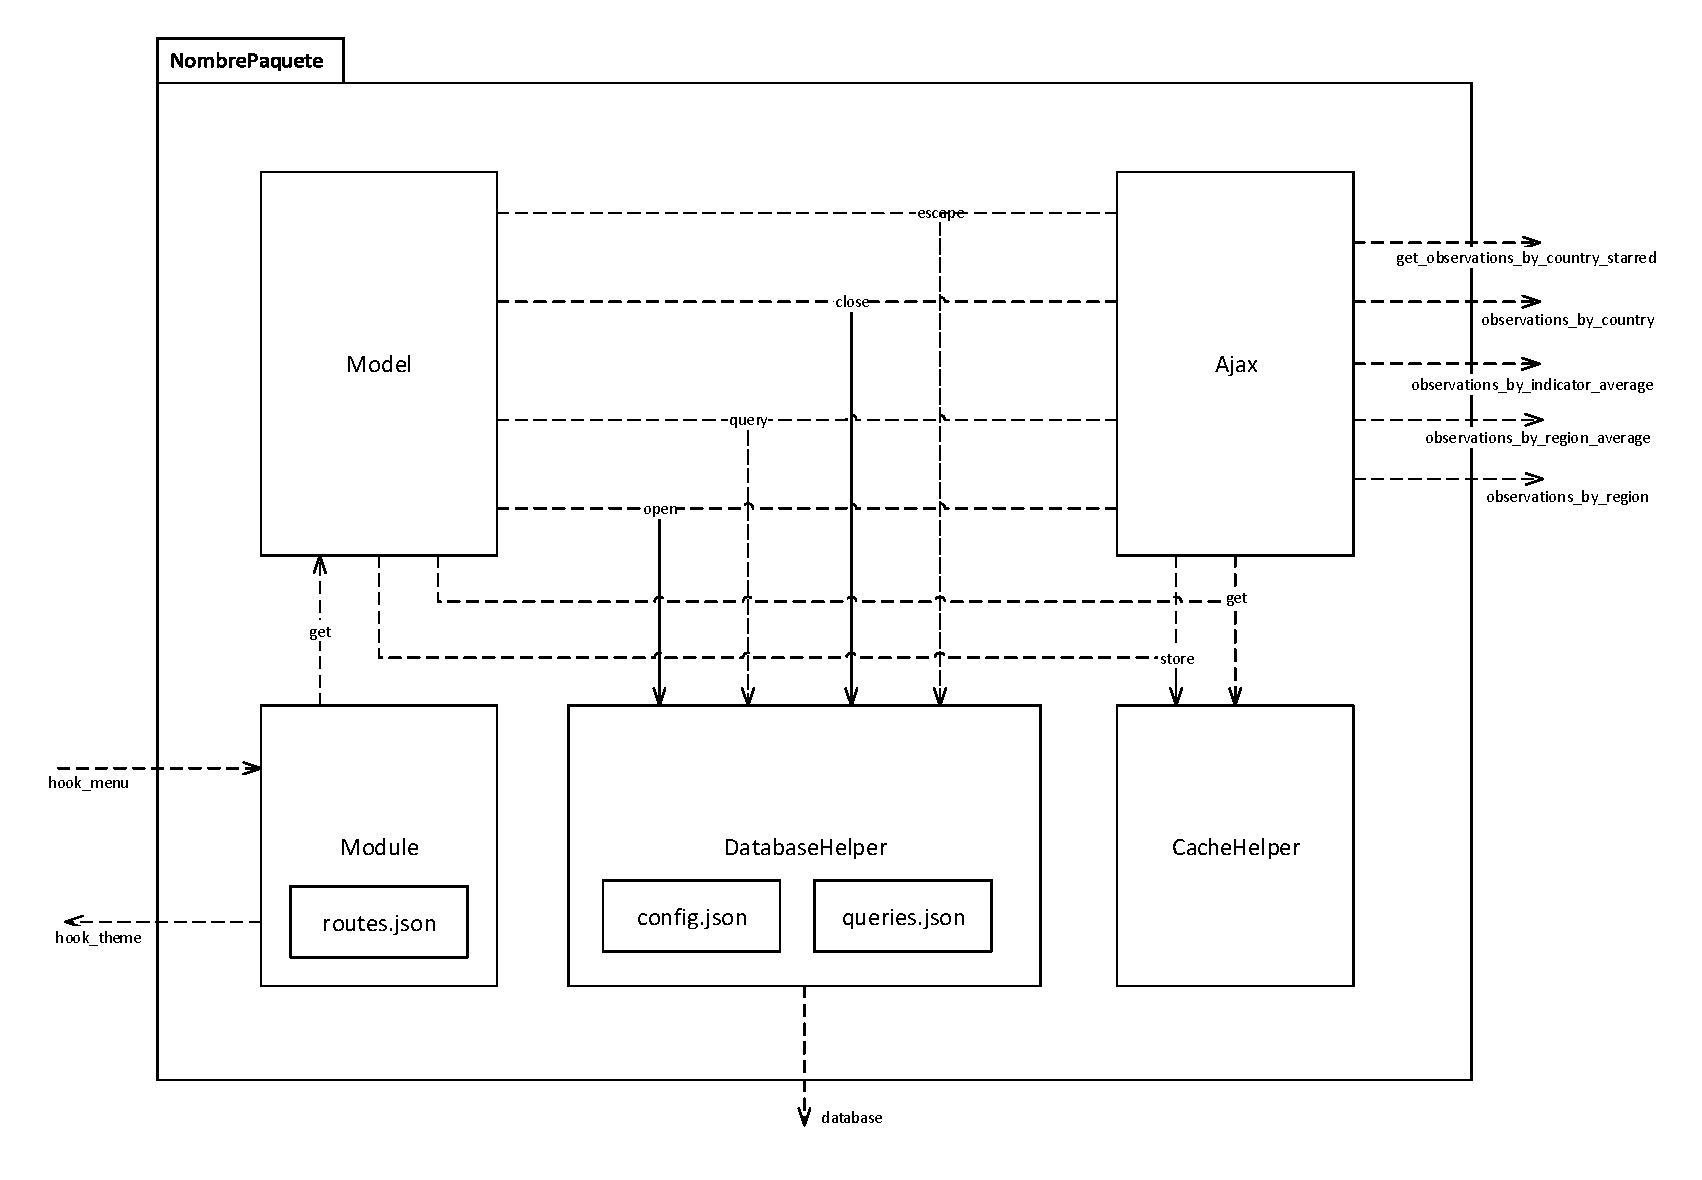
\includegraphics[height=\textwidth]{arquitectura/landportal_uris_view}
		\caption{Diagrama de componentes del módulo ``\textit{landportal\_uris}''}
		\label{fig:diagrama_componentes_landportal_uris}
	\end{figure}
\end{landscape}


\subsubsection{Descripción de los componentes}
Se describirán ahora los distintos componentes que forman parte del módulo ``\textit{landportal\_uris}''.  La organización de dichos componentes puede verse en la figura \ref{fig:diagrama_componentes_landportal_uris}
\begin{description}
	\item[Module]  Contiene la implementación del \textit{hook} que el gestor de contenidos utilizará para llamar a éste módulo.  Es el principal punto de entrada al módulo.  Incluye un fichero donde se declararán las rutas y las vistas que estarán disponibles.
	\item[DatabaseHelper]  Funciona como una capa de abstracción sobre la base de datos.  Ofrece una serie de métodos que serán utilizados por el resto de componentes que necesiten acceder a la base de datos.  Incluye un fichero que configura la información de conexión a la base de datos y otro que incluye las consultas disponibles.
	\item[CacheHelper]  Permite el cacheo de datos con el fin de agilizar la consulta y procesado de grandes cantidades de datos.  Ofrece una serie de métodos que serán utilizados por el resto de componentes que necesiten acceder al caché.
	\item[Ajax]  Implementa el framewok que da soporte a la creación de visualizaciones.  Expone varias interfaces que serán utilizadas por las visualizaciones para obtener los datos que posteriormente presentarán a los usuarios.
	\item[Model]  Devuelve los datos necesarios para presentar las diferentes vistas del sistema.  Los modelos se invocarán utilizando un convenio de nombres en función de la vista a la que pertencezcan.
\end{description}

\subsubsection{Relación entre los componentes}
El módulo lee la configuración de rutas desde el fichero ``\textit{routes.json}''.  Con cada petición recibida desde el núcleo del gestor de contenidos se buscará el modelo correspondiente a la vista mediante un convenio de nombres y se invocará su funcionalidad.  Posteriormente se invocará al tema para que renderice la vista adecuada.

Los modelos cargarán los datos necesarios para la renderización de la vista a través de diferentes consultas a la base de datos.  
El framework de soporte a visualizaciones funcionará de forma similar a los modelos, realizando consultas a la base de datos para obtener los datos necesarios.

En ambos casos, para agilizar la consulta y el procesamiento de los datos, los resultados se cachearán antes de ser devueltos, de forma que las posteriores peticiones accedan directamente a la información del caché.


\subsubsection{Interfaces y puertos}
A continuación se detallarán las interfaces y puertos de los componentes que forman parte del módulo ``\textit{landportal\_uris}''.

\paragraph{LandPortal URIs} \hfill \\
La tabla \ref{interfaces_landportal_uris_landportal_uris} muestra el detalle de las interfaces del módulo ``\textit{LandPortal URIs}''.  

\begin{longtable}[c]{|p{25mm}|p{20mm}|p{30mm}|p{60mm}|}
	\caption{Vista del módulo \textit{LandPortal URIs}- interfaces del módulo \textit{LandPortal URIs}. \label{interfaces_landportal_uris_landportal_uris}}\\
	%Cabecera en la primera pagina
		\hline
			Interfaz & Tipo & Tecnología & Propiedades\\
		\hline
		\hline
	\endfirsthead
	%Cabecera en el resto de páginas
		\hline
		\multicolumn{4}{|c|}{Continuación de la tabla \ref{interfaces_landportal_uris_landportal_uris}}\\
		\hline
			Interfaz & Tipo & Tecnología & Propiedades\\
		\hline
		\hline
	\endhead
	%Tabla
	\hline
	\endfoot
		\textbf{hook menu} & Proveída & Llamada a método & Invocado por el gestor de contenidos durante la definición de las rutas que tendrán las vistas del portal \\
		\hline
		\textbf{hook theme} & Requerida & Llamada a método & Pide al tema que renderice una determinada plantilla para una vista \\
		\hline
		\textbf{get observations by country starred} & Proveída & API Web & Devuelve todas las observaciones referentes a un determinado país para los indicadores favoritos \\
		\hline
		\textbf{observations by country} & Proveída & API Web & Devuelve todas las observaciones referentes a un determinado país sin tener en cuenta el indicador \\
		\hline
		\textbf{get observations by indicator average} & Proveída & API Web & Devuelve el valor medio de todas las observaciones para un determinado indicador \\
		\hline
		\textbf{get observations by region average} & Proveída & API Web & Devuelve el valor medio de todas las observaciones referente a una determinada región sin tener en cuenta el indicador \\
		\hline
		\textbf{observations by region} & Proveída & API Web & Devuelve todas las observaciones referentes a una determinada región sin tener en cuenta el indicador \\
		\hline
		\textbf{database} & Requerida & Conexión a base de datos & Obtiene información de la base de datos \\
	\hline
	\hline
\end{longtable}

\paragraph{Module} \hfill \\
La tabla \ref{interfaces_landportal_uris_module} muestra el detalle de las interfaces del componente ``\textit{module}''.  

\begin{longtable}[c]{|p{25mm}|p{20mm}|p{30mm}|p{60mm}|}
	\caption{Vista del módulo \textit{LandPortal URIs}- interfaces del componente ``\textit{module}''. \label{interfaces_landportal_uris_module}}\\
	%Cabecera en la primera pagina
		\hline
			Interfaz & Tipo & Tecnología & Propiedades\\
		\hline
		\hline
	\endfirsthead
	%Cabecera en el resto de páginas
		\hline
		\multicolumn{4}{|c|}{Continuación de la tabla \ref{interfaces_landportal_uris_module}}\\
		\hline
			Interfaz & Tipo & Tecnología & Propiedades\\
		\hline
		\hline
	\endhead
	%Tabla
	\hline
	\endfoot
		\textbf{hook menu} & Puerto de entrada & Llamada a método & Invocado por el gestor de contenidos durante la definición de las rutas que tendrán las vistas del portal \\
		\hline
		\textbf{hook theme} & Requerida & Llamada a método & Pide al tema que renderice una determinada plantilla para una vista \\
		\hline
		\textbf{get} & Puerto de salida & Llamada a método & Pide a un modelo los datos necesarios para que posteriormente el tema renderice la vista \\
		\hline
	\hline
	\hline
\end{longtable}


\paragraph{DatabaseHelper} \hfill \\
La tabla \ref{interfaces_landportal_uris_databasehelper} muestra el detalle de las interfaces del componente ``\textit{DatabaseHelper}''.  

\begin{longtable}[c]{|p{25mm}|p{20mm}|p{30mm}|p{60mm}|}
	\caption{Vista del módulo \textit{LandPortal URIs}- interfaces del componente ``\textit{DatabaseHelper}''. \label{interfaces_landportal_uris_databasehelper}}\\
	%Cabecera en la primera pagina
		\hline
			Interfaz & Tipo & Tecnología & Propiedades\\
		\hline
		\hline
	\endfirsthead
	%Cabecera en el resto de páginas
		\hline
		\multicolumn{4}{|c|}{Continuación de la tabla \ref{interfaces_landportal_uris_databasehelper}}\\
		\hline
			Interfaz & Tipo & Tecnología & Propiedades\\
		\hline
		\hline
	\endhead
	%Tabla
	\hline
	\endfoot
		\textbf{open} & Puerto de entrada & Llamada a método & Abre una conexión con la base de datos \\
		\hline
		\textbf{query} & Puerto de entrada & Llamada a método & Realiza una consulta a la base de datos y devuelve su resultado \\
		\hline
		\textbf{close} & Puerto de entrada & Llamada a método & Cierra una conexión con la base de datos \\
		\hline
		\textbf{escape} & Puerto de entrada & Llamada a método & Escapa los parámetros de una consulta antes de enviarla a la base de datos\footnote{El escapado de argumentos es un procedimiento necesario para evitar ataques del tipo \textit{SQLInjection} cuando no se utilizan \textit{PreparedStatements}.  Para más información al respecto véase \url{http://www.php.net/manual/en/mysqli.real-escape-string.php}} \\
		\hline
		\textbf{database} & Puerto de salida & Conexión a base de datos & Obtiene información de la base de datos \\
	\hline
	\hline
\end{longtable}


\paragraph{CacheHelper} \hfill \\
La tabla \ref{interfaces_landportal_uris_cachehelper} muestra el detalle de las interfaces del componente ``\textit{CacheHelper}''.  

\begin{longtable}[c]{|p{25mm}|p{20mm}|p{30mm}|p{60mm}|}
	\caption{Vista del módulo \textit{LandPortal URIs}- interfaces del componente ``\textit{CacheHelper}''. \label{interfaces_landportal_uris_cachehelper}}\\
	%Cabecera en la primera pagina
		\hline
			Interfaz & Tipo & Tecnología & Propiedades\\
		\hline
		\hline
	\endfirsthead
	%Cabecera en el resto de páginas
		\hline
		\multicolumn{4}{|c|}{Continuación de la tabla \ref{interfaces_landportal_uris_cachehelper}}\\
		\hline
			Interfaz & Tipo & Tecnología & Propiedades\\
		\hline
		\hline
	\endhead
	%Tabla
	\hline
	\endfoot
		\textbf{get} & Puerto de entrada & Llamada a método & Obtiene el elemento almacenado en el caché bajo una determinada clave \\
		\hline
		\textbf{store} & Puerto de entrada & Llamada a método & Almacena un elemento en el caché utilizando una determinada clave que posteriormente podrá ser utilizada para recuperarlo \\
		\hline
	\hline
	\hline
\end{longtable}

\paragraph{Model} \hfill \\
La tabla \ref{interfaces_landportal_model} muestra el detalle de las interfaces comunes a todos los modelos.  

\begin{longtable}[c]{|p{25mm}|p{20mm}|p{30mm}|p{60mm}|}
	\caption{Vista del módulo \textit{LandPortal URIs}- interfaces del componente ``\textit{Model}''. \label{interfaces_landportal_model}}\\
	%Cabecera en la primera pagina
		\hline
			Interfaz & Tipo & Tecnología & Propiedades\\
		\hline
		\hline
	\endfirsthead
	%Cabecera en el resto de páginas
		\hline
		\multicolumn{4}{|c|}{Continuación de la tabla \ref{interfaces_landportal_model}}\\
		\hline
			Interfaz & Tipo & Tecnología & Propiedades\\
		\hline
		\hline
	\endhead
	%Tabla
	\hline
	\endfoot
		\textbf{open} & Puerto de salida & Llamada a método & Abre una conexión con la base de datos \\
		\hline
		\textbf{query} & Puerto de salida & Llamada a método & Realiza una consulta a la base de datos y devuelve su resultado \\
		\hline
		\textbf{close} & Puerto de salida & Llamada a método & Cierra una conexión con la base de datos \\
		\hline
		\textbf{escape} & Puerto de salida & Llamada a método & Escapa los parámetros de una consulta antes de enviarla a la base de datos \\
		\hline
		\textbf{get} & Puerto de entrada & Llamada a método & Devuelve la información necesaria para que el tema renderice la vista correspondiente \\
		\hline
		\textbf{get (CacheHelper)} & Puerto de salida & Llamada a método & Obtiene el elemento almacenado en el caché bajo una determinada clave \\
		\hline
		\textbf{store} & Puerto de salida & Llamada a método & Almacena un elemento en el caché utilizando una determinada clave que posteriormente podrá ser utilizada para recuperarlo \\
	\hline
	\hline
\end{longtable}


\paragraph{Ajax} \hfill \\
La tabla \ref{interfaces_landportal_ajax} muestra el detalle de las interfaces pertenecientes al framework de soporte a las visualizaciones.  

\begin{longtable}[c]{|p{25mm}|p{20mm}|p{30mm}|p{60mm}|}
	\caption{Vista del módulo \textit{LandPortal URIs}- interfaces del componente ``\textit{Ajax}''. \label{interfaces_landportal_ajax}}\\
	%Cabecera en la primera pagina
		\hline
			Interfaz & Tipo & Tecnología & Propiedades\\
		\hline
		\hline
	\endfirsthead
	%Cabecera en el resto de páginas
		\hline
		\multicolumn{4}{|c|}{Continuación de la tabla \ref{interfaces_landportal_ajax}}\\
		\hline
			Interfaz & Tipo & Tecnología & Propiedades\\
		\hline
		\hline
	\endhead
	%Tabla
	\hline
	\endfoot
		\textbf{open} & Puerto de salida & Llamada a método & Abre una conexión con la base de datos \\
		\hline
		\textbf{query} & Puerto de salida & Llamada a método & Realiza una consulta a la base de datos y devuelve su resultado \\
		\hline
		\textbf{close} & Puerto de salida & Llamada a método & Cierra una conexión con la base de datos \\
		\hline
		\textbf{escape} & Puerto de salida & Llamada a método & Escapa los parámetros de una consulta antes de enviarla a la base de datos \\
		\hline
		\textbf{get (CacheHelper)} & Puerto de salida & Llamada a método & Obtiene el elemento almacenado en el caché bajo una determinada clave \\
		\hline
		\textbf{store} & Puerto de salida & Llamada a método & Almacena un elemento en el caché utilizando una determinada clave que posteriormente podrá ser utilizada para recuperarlo \\
		\hline
		\textbf{get observations by country starred} & Puerto de salida & API Web & Devuelve todas las observaciones referentes a un determinado país para los indicadores favoritos \\
		\hline
		\textbf{observations by country} & Puerto de salida & API Web & Devuelve todas las observaciones referentes a un determinado país sin tener en cuenta el indicador \\
		\hline
		\textbf{get observations by indicator average} & Puerto de salida & API Web & Devuelve el valor medio de todas las observaciones para un determinado indicador \\
		\hline
		\textbf{get observations by region average} & Puerto de salida & API Web & Devuelve el valor medio de todas las observaciones referente a una determinada región sin tener en cuenta el indicador \\
		\hline
		\textbf{observations by region} & Puerto de salida & API Web & Devuelve todas las observaciones referentes a una determinada región sin tener en cuenta el indicador \\
		\hline
	\hline
	\hline
\end{longtable}

%\section{Comportamiento del sistema}
%\label{comportamiento_sistema}

\section{Diseño de la base de datos}
\label{diseno_base_datos}

\section{Diseño de la interfaz de usuario}
\label{diseno_interfaz_usuario}

\chapter{Implementación del sistema}
\label{chapter:implementacion}
En éste capítulo se detallarán los aspectos más importantes de la implementación del sistema, desde los lenguajes de programación y herramientas utilizadas hasta los principales problemas surgidos durante el desarrollo y sus soluciones.


\section{Lenguajes de programación utilizados}
\label{implementacion:lenguajes_programacion}
	
	A continuación se describirán los lenguajes de programación utilizados y sus respectivas versiones.
	\begin{description}
		\item[PHP]
			Para el desarrollo de los módulos pertenecientes al gestor de contenidos, así como las plantillas del tema visual, se ha utilizado el lenguaje PHP (\textit{PHP: Hypertext Preprocessor}).  La versión del lenguaje PHP utilizada es la 5.5\footnote{La versión 5.5 del lenguaje PHP incluye, entre otras características, soporte a generadores y capacidad de iteración por cualquier tipo de clave (no sólo numérica) en los bucles \textit{foreach}.  Para una mayor información al respecto se recomienda leer el anuncio oficial en \url{http://php.net/releases/5_5_0.php}}.  La única extensión de PHP utilizada ha sido APC (\textit{Alternative PHP Cache}), que permite cachear y optimizar el código intermedio de PHP con el objetivo de aumentar el rendimiento siempre que sea posible, el uso de éste caché puede verse descrito en la sección ``\nameref{actividad:framework_visualizaciones}'' perteneciente al capítulo \ref{chapter05}.
		\item[Python]
			Para el desarrollo del Punto de Entrada de Datos (o \textit{Receiver}) se ha utilizado el lenguaje Python en su versión 2.7. Se ha decidido utilizar la versión 2.7 de Python debido a que las versiones 3.x contienen varias incompatibilidades con las anteriores versiones, éstas incompatibilidades provocan que la existencia de librerías externas sea más reducida.  En el PEP (\textit{Python Enhancement Proposal}) 373\footnote{El PEP 373 está disponible para su consulta en \url{http://legacy.python.org/dev/peps/pep-0373/}} se establece que la versión 2.7 de Python estará soportada hasta el año 2020.  En la posterior sección ``\nameref{implementacion:herramientas_utilizadas}'' se explicarán las herramientas que se han utilizado para aislar el entorno y gestionar las dependencias externas.
		\item[SQL]
			Para interactuar con la base de datos se ha utilizado el lenguaje SQL, Cabe destacar que todas las consultas realizadas se adhieren a la especificación de SQL estándar y no utilizan características propias de ningún sistema de gestión de bases de datos.
		\item[Otros]
			A pesar de no ser lenguajes de programación como tal, también se incluirán algunos lenguajes que se han utilizado en varias partes del sistema.
			\begin{itemize}
				\item \textbf{XML}
					Para el intercambio de datos entre los Importadores y el Punto de Entrada de Datos se ha utilizado el lenguaje de marcas XML (\textit{Extensible Markup Language}).  A pesar de la existencia de otros lenguajes con un objetivo similar (JSON es uno de ellos y se verá a continuación) se ha decidido utilizar XML para ésta tarea por su capacidad para validar la estructura del documento contra un esquema dado.
				\item \textbf{JSON}
					Para el envío de datos a las vistas y visualizaciones se ha utilizado el formato JSON (\textit{JavaScript Object Notation}).  Se ha escogido JSON por ser un formato mucho más ligero que XML.  Además, puesto que en éstos casos los datos provienen desde dentro del sistema su integridad está garantizada.
						\begin{itemize}
							\item
								El formato JSON también se ha utilizado para albergar varios ficheros de configuración, como se puede ver en la ``\nameref{vista_landportal_uris}''.  A pesar de la existencia de otros formatos como YAML (\textit{YAML Ain't Markup Language}) se ha decidido utilizar JSON por consistencia con el resto de partes del sistema.
						\end{itemize}
				\item \textbf{HTML y CSS}
					Toda la interfaz web del portal se ha desarrollado utilizando el lenguaje HTML 5 para crear el contenido de las diferentes páginas, así como el lenguaje CSS 3 para dar estilo visual a las mismas.
			\end{itemize}
	\end{description}


\section{Herramientas utilizadas}
\label{implementacion:herramientas_utilizadas}

A continuación se describirán las herramientas utilizadas durante el desarrollo del sistema.
\begin{description}
	\item[PyCharm]
		Para el desarrollo del Punto de Entrada de Datos se ha utilizado el entorno de desarrollo integrado PyCharm en su versión 3.3 y 3.4.  PyCharm es un IDE para el desarrollo en lenguaje Python desarrollado por JetBrains\footnote{\url{http://www.jetbrains.com/pycharm/}}.
	\item[Editor de texto]
		Para el desarrollo del código PHP que forma parte de los módulos de Drupal se ha utilizado en primer lugar el editor de texto Sublime Text 2\footnote{\url{http://www.sublimetext.com/2}} y posteriormente el editor Atom\footnote{\url{https://atom.io/}}.  Se ha decidido cambiar desde Sublime Text a Atom debido a ser éste último un producto de código abierto, gratuito y con un ritmo de desarrollo muy activo.
	\item[VirtualEnv]
		Se ha utilizadoo la herramienta VirtualEnv\footnote{\url{http://virtualenv.readthedocs.org/en/latest/virtualenv.html}} para crear entornos de Python aislados.  Utilizar entornos aislados permite instalar librerías y paquetes sin que colisionen entre los diferentes entornos existentes, también permite mantener múltiples intérpretes de Python funcionando de forma simultánea.
	\item[PIP]
		En conjunción con la herramienta VirtualEnv mencionada anteriormente, también se ha utilizado la herramienta PIP\footnote{\url{https://pypi.python.org/pypi/pip}} para gestionar los distintos paquetes y dependencias.  PIP permite descargar e instalar de forma automática paquetes externos junto a sus dependencias, también permite especificar todas las dependencias en un único fichero de texto.
	\item[Git y GitHub]
		Durante todo el desarrollo se ha utilizado Git\footnote{\url{http://www.git-scm.com/}} como sistema de control de versiones.  En conjunción con Git, se ha utilizado GitHub\footnote{\url{https://github.com/}} como \textit{hosting} para los distintos repositorios que forman parte del sistema.
\end{description}


\section{Problemas encontrados}
\label{implementacion:problemas_encontrados}
	
	Se describirán a continuación los problemas técnicos encontrados durante el desarrollo del sistema y las soluciones que se han dado a cada uno de ellos.
	
	\subsection{Internacionalización de datos}
	\label{implementacion:internacionalizacion_datos}
		
		Como ya se explicó en la sección ``\nameref{requisitos_seccion_datos}'', no sólo era necesario internacionalizar las vistas del sistema si no también los propios datos.  La internacionalización de los datos supuso un gran reto durante la construcción del sistema, puesto que requirió ser soportada por todas las partes que lo componen.
		
		La solución para la internacionalización de los datos consistió en (como se puede ver en la sección ``\nameref{diseno_modelo_datos}'' perteneciente al capítulo \ref{chapter05}) la creación de varias clases en el modelo de datos destinadas al almacenamiento de las traducciones en diferentes idiomas.  Como contrapunto a esta solución, el modelo de datos adquirió una gran complejidad, con 30 clases diferentes.  Los problemas derivados de esta complejidad se detallarán en el punto siguiente.
	
	\subsection{Complejidad del modelo de datos}
	\label{implementacion:internacionalizacion_datos}
		
		Tal y como se mencionó en el punto anterior y se puede comprobar en la sección ``\nameref{diseno_modelo_datos}'' el modelo de datos adquirió una gran complejidad, alcanzando las 30 clases diferentes.
		
		Ésta complejidad proviene principalmente de la necesidad de cumplir con la especificación del vocabulario RDF Data Cube (éste concepto fue explicado en detalle en la sección \ref{concept:rdf_data_cube} perteneciente al capítulo ``\nameref{chapter03}'') y de la necesidad de internacionalizar los datos del sistema.
		
		La solución a éste problema consistió en asumir dicha complejidad y tenerla siempre presente para optimizar la inserción y la extracción de datos en la medida de lo posible.
		
	\subsection{Importación de datos}
	\label{implementacion:importacion de datos}
		
		La implementación de la importación de datos en el sistema fue problemática debido a la necesidad de soportar la entrada de grandes conjuntos de datos.  Algunas fuentes de datos incluyen catálogos de datos de unos 40mb en formato de texto plano sin espacios ni saltos de líneas.
		
		Debido a ésta cantidad de información fue necesario tomar algunas medidas para hacer más efectivo el proceso de importación.  A continuación se explicará que soluciones se tomaron al respecto.
		\begin{itemize}
			\item
				Uso de nu nuevo módulo para el parseo de los ficheros entrantes.  Python cuenta con dos implementaciones del parser XML de su librería estándar\footnote{El parser recibe el nombre de \textit{ElementTree}.  Para más información véase la entrada en la documentación oficial de Python al respecto en \url{https://docs.python.org/2/library/xml.etree.elementtree.html}}: una de ellas en lenguaje Python y la otra en lenguaje C.  Puesto que ambas implementaciones tienen la misma interfaz, pueden intercambiarse de forma transparente.  Usar la implementación en lengaje C del parser permitió aumentar la velocidad y reducir el consumo de memoria del proceso de importación de datos.
			\item
				Uso de generadores.  El uso de listas hace necesario mantener grandes cantidades de objetos de forma simultánea en la memoria.  La utilización de generadores permite que los objetos sean devueltos bajo demanda y, por tanto, los objetos no utilizados pueden ser eliminados por el recolector de basura con la consiguiente reducción en el uso de memoria.
			\item
				Inserciones parciales.  Con grandes cantidades de datos las consultas de inserción en la base de datos producen que el SGBD\footnote{Como se detalló en la sección ``\nameref{chapter02:alternativas_seleccionadas}'' perteneciente al capítulo \ref{chapter02}, el Sistema de Gestión de Bases de Datos utilizado es MySQL.} falle al no poder gestionar tanta información.  La realización de varias inserciones parciales en las que sólo se inserta un determinado número de objetos, en lugar de una única gran inserción permitió eliminar éste problema.
		\end{itemize}
		
	\subsection{Adaptación al CMS}
	\label{implementacion:adaptacion_cms}
	
		El desarrollo de los módulos de Drupal que se pueden ver en la sección ``\nameref{vista_modulos_cms}'' perteneciente al capítulo \ref{chapter05} requirió adaptar el desarrollo a las técnicas y mecanismos utilizados por el gestor de contenidos y, en muchas ocasiones, luchar contra el propio CMS para realizar algunas tareas.
		
		La solución a éste problema consistió en utilizar extensivamente la documentación oficial de Drupal\footnote{La documentación oficial de Drupal puede consultarse en \url{https://www.drupal.org/documentation}} intentar comprender al máximo posible su funcionamiento para, de ésta forma, intentar reducir al mínimo dichas situaciones.



\chapter{Desarrollo de las pruebas}
\label{chapter:desarrollo_pruebas}
En éste capítulo se detallarán las pruebas que se han realizado durante el desarrollo del proyecto así como los resultados de las mismas.


\section{Pruebas de integración}
\label{pruebas:integracion}
	
	
	\subsection{Casos de prueba de la zona de datos}
	\label{pruebas:integracion:zona_datos}
	Como se ha explicado anteriormente en la sección ``\nameref{especificacion_plan_pruebas}'' perteneciente al capítulo \ref{chapter04}, el subsistema de datos se ha desarrollado utilizando una metodología de Desarrollo Dirigido por Pruebas acompañada de un proceso de integración continua.  A continuación se explicará la forma en la que se han aplicado las pruebas y los beneficios que han aportado al proceso de desarrollo.

\subsubsection{Desarrollo Dirigido por Pruebas}
	El Desarrollo Dirigido por Pruebas (o \textit{Test Driven Development}) consiste en repetir los siguientes pasos continuamente durante el proceso de desarrollo del sistema:
	\begin{enumerate}
		\item
			Antes de añadir una nueva funcionalidad escribir una o varias pruebas para ella.  Las pruebas fallarán hasta que la funcionalidad en cuestión no esté implementada.
		\item
			Implementar la funcionalidad hasta que pase correctamente las pruebas diseñadas anteriormente.
		\item
			Refactorizar el código cuando sea necesario.  Puesto que las pruebas ya están escritas, se puede comprobar rápidamente si la refactorización ha introducido nuevos errores en el código.
	\end{enumerate}
	
	Las ventajas que ha aportado el uso de esta metodología durante el desarrollo se detallarán a continuación:
	\begin{itemize}
		\item
			En muchas ocasiones las pruebas se realizan únicamente al final del desarrollo del software, lo que provoca que estas sean ineficientes e incompletas.  La obligación de escribir las pruebas antes que la propia funcionalidad revierte esta situación y asegura la existencia de las pruebas (la corrección y completitud de las mismas queda siempre en manos del desarrollador).
		\item
			Pensar en las pruebas previamente a la implementación hace más fácil encontrar posibles situaciones extrañas que puedan provocar problemas en el sistema.
		\item
			Dado que las pruebas actúan como los primeros clientes del código, existe una cierta obligación a hacer que la implementación real tenga una interfaz más definida y consistente.
		\item
			La existencia de las pruebas ayuda a aumentar la confianza durante las refactorizaciones de código.  Esto ha sido especialmente útil dado que el lenguaje utilizado para el desarrollo del subsistema de datos ha sido Python, cuya dinamicidad aporta en muchas ocasiones menos seguridad que otros más estáticos.
	\end{itemize}
	
\subsubsection{Integración continua}
	Con el objetivo de automatizar el proceso de pruebas y notificar al equipo de desarrollo de posibles fallos en los casos de prueba que hayan podido pasar desapercibidos, las pruebas descritas en el punto anterior se acompañan de la ayuda de un servidor de integración continua.
	
	Una posible definición de integración continua, extraída de \cite{mfowler:continuous-integration} es la siguiente:
	\begin{quote}
		``\textit{Continuous Integration is a software development practice where members of a team integrate their work frequently, usually each person integrates at least daily - leading to multiple integrations per day. Each integration is verified by an automated build (including test) to detect integration errors as quickly as possible.}''
	\end{quote}}
	
	Por su utilidad y su capacidad de integración con GitHub (plataforma de control de versiones con la que se desarrolló este proyecto) se ha utilizado el servidor de integración continua Travis-CI\footnote{\url{https://travis-ci.org/}}.  
	
	La siguiente cita de Martin Fowler \cite{mfowler:continuous-integration} puede ayudar al lector a comprender la funcionalidad de este tipo de servidores:
	\begin{quote}
		``\textit{A continuous integration server acts as a monitor to the repository. Every time a commit against the repository finishes the server automatically checks out the sources onto the integration machine, initiates a build, and notifies the committer of the result of the build. The committer isn't done until she gets the notification - usually an email.}''
	\end{quote}
	
	Las principales ventajas que ha aportado el uso de un servidor de integración continua como Travis-CI al proceso de desarrollo han sido varias, entre las que destacan:
	\begin{itemize}
		\item
			El servidor de integración continua asegura que las pruebas se ejecutarán ante cualquier cambio del código que se produzca en el repositorio.
		\item
			En caso de que surga algún fallo durante la ejecución de las pruebas, el servidor de integración continua notifica al autor de los cambios que lo producen.  Esta capacidad de notificación prácticamente inmediata ha ayudad a detectar y solucionar varios problemas de forma rápida antes de que se propaguen a otras partes del sistema.
	\end{itemize}
	
	
	\subsection{Casos de prueba de la zona social}
	\label{pruebas:integracion:zona_social}
	A continuación se presentarán los diferentes casos de prueba realizados sobre los subsistemas pertenecientes a la zona zona social (subsistema de gestión de usuarios, noticias, debates, eventos, blog, organizaciones, comentarios y búsqueda).  Cada caso de prueba cuenta con una descripción, el resultado esperado en la ejecución y el resultado obtenido.

Los fallos encontrados durante ésta fase han sido corregidos antes de entregar la versión final del sistema.

\subsubsection{Subsistema de gestión de usuarios}
La tabla \ref{table:casos_prueba_usuarios} muestra los casos de prueba del subsistema de gestión de usuarios.


\begin{landscape}
	\begin{longtable}[c]{|p{50mm}|p{50mm}|p{50mm}|p{50mm}|}
	 \caption{Casos de prueba del subsistema de gestión de usuarios\label{table:casos_prueba_usuarios}}\\
	
	 %Cabecera en la primera pagina
	 \hline
	 \multicolumn{4}{|c|}{\textbf{Casos de prueba del subsistema de gestión de usuarios}}\\
	 \hline
	 \textbf{Descripción} & \textbf{Proceso de prueba} & \textbf{Resultado esperado} & \textbf{Resultado obtenido}\\
	 \hline
	 \hline
	 \endfirsthead
	 
	 %Cabecera en el resto de páginas
	 \hline
	 \multicolumn{4}{|c|}{Continuación de la tabla \ref{table:casos_prueba_usuarios}}\\
	 \hline
	 \textbf{Descripción} & \textbf{Proceso de prueba} & \textbf{Resultado esperado} & \textbf{Resultado obtenido}\\
	 \hline
	 \hline
	 \endhead
	 
	 \hline
	 \endfoot
	 
	Registrar un nuevo usuario con un nombre y email no existentes en el sistema & Acceder al formulario de registro e introducir los como nombre de usuario ``\textit{prueba}'' y como email ``\textit{prueba@example.com}''.  El resto de campos pueden tener cualquier valor siempre que se rellenen los campos obligatorios & La nueva cuenta de usuario se crea correctamente y con estado bloqueado & Resultado esperado\\
	\hline
	Registrar un nuevo usuario con un nombre ya existente en el sistema & Acceder al formulario de registro e introducir como nombre de usuario ``\textit{prueba}'' y como email ``\textit{prueba2@example.com}''.  El resto de campos pueden tener cualquier valor siempre que se rellenen los campos obligatorios & El sistema no crea la cuenta de usuario y notifica de que el nombre no puede utilizarse & Resultado esperado\\
	\hline
	Registrar un nuevo usuario con un email ya existente en el sistema & Acceder al formulario de registro e introducir como nombre de usuario ``\textit{prueba2}'' y como email ``\textit{prueba@example.com}''.  El resto de campos pueden tener cualquier valor siempre que se rellenen los campos obligatorios & El sistema no crea la cuenta de usuario y notifica de que el email no puede utilizarse & Resultado esperado\\
	\hline
	Registrar un nuevo usuario con un nombre inválido & Acceder al formulario de registro e introducir como nombre de usuario ``\textit{prueba,3}'' y como email ``\textit{prueba3@example.com}''.  El resto de campos pueden tener cualquier valor siempre que se rellenen los campos obligatorios & El sistema no crea la cuenta de usuario y notifica de que el nombre contiene caracteres incorrectos & Resultado esperado\\
	\hline
	Registrar un nuevo usuario con un email inválido & Acceder al formulario de registro e introducir como nombre de usuario ``\textit{prueba3}'' y como email ``\textit{correofalso}''.  El resto de campos pueden tener cualquier valor siempre que se rellenen los campos obligatorios & El sistema no crea la cuenta de usuario y notifica de que el email tiene un formato inválido & Resultado esperado\\
	\hline
	Registrar un nuevo usuario sin rellenar todos los campos obligatorios & Acceder al formulario de registro e introducir como email ``\textit{prueba3@example.com}''. El resto de campos puede tener cualquier valor salvo el nombre, que se dejará en blanco & El sistema no crea la cuenta de usuario y notifica de que el nombre debe ser introducido & Resultado esperado\\
	\hline
	Iniciar sesión en el sistema con un usuario bloqueado & Acceder al formulario de login e intentar iniciar sesión con el usuario ``\textit{prueba}'' & El sistema no permite el inicio de sesión puesto que el usuario está bloqueado & Resultado esperado. \\
	\hline
	Activar un usuario bloqueado & Acceder a la vista de administración y activar al usuario ``\textit{prueba}'', que se encuentra bloqueado & El sistema cambiará el estado del usuario y enviará un correo indicándole que establezca su contraseña para iniciar sesión en el sistema & Falla.  Se produce un error al enviar el correo electrónico, aunque el estado del usuario se cambia a activo correctamente\\
	\hline
	Iniciar sesión en el sistema con un usuario activado & Acceder al formulario de login e introducir como nombre ``\textit{prueba}'' y como contraseña la que haya establecido el usuario & El sistema permite iniciar sesión correctamente al usuario & Resultado esperado\\
	\hline
	Iniciar sesión en el sistema con campos vacíos & Acceder al formulario de login e introducir como nombre ``\textit{prueba}'', dejar el campo contraseña vacío e iniciar sesión & El sistema no permitirá iniciar sesión por haber dejado campos vacíos en el formulario & Resultado esperado\\
	\hline
	Iniciar sesión en el sistema con una contraseña incorrecta & Acceder al formulario de login e introducir como nombre ``\textit{prueba}'' y como contraseña un diferente a la escogida por el usuario & El sistema no permitirá iniciar sesión porque la contraseña es incorrecta & Resultado esperado\\
	\hline
	Un usuario anónimo accede al perfil de un usuario registrado & Sin haber iniciado sesión en el sistema acceder a la vista de perfil de un usuario registrado & El sistema no permite que los usuarios anónimos vean los perfiles de los usuarios registrados y mostrará la página de error & Resultado esperado\\
	\hline
	Un usuario registrado accede al perfil de otro usuario registrado & Habiendo iniciado sesión en el sistema acceder a la vista de perfil de un usuario registrado & El sistema mostrará los datos del perfil del usuario & Resultado esperado\\
	\hline
	Un usuario registrado accede al perfil de otro usuario con capacidad de acceso al API & Habiendo iniciado sesión en el sistema acceder a la vista de perfil de un usuario con capacidad de acceso al API & El sistema mostrará los datos del perfil del usuario excepto la clave de acceso al API & Resultado esperado\\
	\hline
	Un usuario registrado accede a su perfil & Habiendo iniciado sesión en el sistema acceder a la vista del propio perfil & El sistema mostrará los datos del usuario e incluirá un botón para editar la información de su perfil & Resultado esperado\\
	\hline
	Un usuario con capacidad de acceso al API accede a su perfil & Habiendo iniciado sesión en el sistema con una cuenta de usuario que tenga capacidad de acceso al API acceder a la vista del propio perfil & El sistema mostrará los datos del usuario incluyendo la clave de acceso al API y un botón para editar la información del perfil & Resultado esperado\\
	\hline
	Un usuario cierra sesión en el sistema & Habiendo iniciado sesión en el sistema pulsar el botón para cerrar sesión & El sistema cerrará la sesión del usuario y redirigirá a la página de inicio del portal & Resultado esperado\\
	\hline
	Dar permisos de acceso al API a un usuario registrado & Habiendo iniciado sesión como administrador acceder a la vista de usuarios del sistema y modificar el rol de un usuario registrado para darle permisos de acceso al API & Cuando el usuario modificado inicie sesión y acceda a la vista de su perfil podrá ver su clave de acceso al API junto con el resto de sus datos & Resultado esperado\\
	\hline
	Dar permisos de administración a un usuario registrado & Habiendo iniciado sesión como administrador acceder a la vista de usuarios del sistema y modificar el rol de un usuario registrado para darle permisos de administración & Cuando el usuario modificado inicie sesión podrá ver la barra superior de administración y realizar las tareas reservadas para el rol de administrador del sistema & Resultado esperado\\
	\hline
	\hline
	
	 \end{longtable}
\end{landscape}

\begin{landscape}
	\subsubsection{Subsistema de gestión de entradas del blog}
	La tabla \ref{table:casos_prueba_blog} muestra los casos de prueba del subsistema de gestión de entradas del blog.
	
	\begin{longtable}[c]{|p{50mm}|p{50mm}|p{50mm}|p{50mm}|}
	 \caption{Casos de prueba del subsistema de gestión de entradas del blog\label{table:casos_prueba_blog}}\\
	
	 %Cabecera en la primera pagina
	 \hline
	 \multicolumn{4}{|c|}{\textbf{Casos de prueba del subsistema de gestión de entradas del blog}}\\
	 \hline
	 \textbf{Descripción} & \textbf{Proceso de prueba} & \textbf{Resultado esperado} & \textbf{Resultado obtenido}\\
	 \hline
	 \hline
	 \endfirsthead
	 
	 %Cabecera en el resto de páginas
	 \hline
	 \multicolumn{4}{|c|}{Continuación de la tabla \ref{table:casos_prueba_blog}}\\
	 \hline
	 \textbf{Descripción} & \textbf{Proceso de prueba} & \textbf{Resultado esperado} & \textbf{Resultado obtenido}\\
	 \hline
	 \hline
	 \endhead
	 
	 \hline
	 \endfoot
	 
	Crear una nueva entrada en el blog como administrador & Habiendo iniciado sesión en el portal como administrador acceder a la vista del blog y pulsar el botón para crear una nueva entrada.  Rellenar el formulario de creación de una entrada sin dejar ningún campo obligatorio en blanco y guardar los cambios & La nueva entrada aparece como la más reciente del blog y los usuarios pueden acceder a ella & Resultado esperado\\
	\hline
	Crear una nueva entrada en el blog sin ser administrador & Habiendo iniciado sesión en el portal como un usuario sin privilegios de administración acceder a la vista del blog e intentar crear una nueva entrada & El botón para crear una nueva entrada no se mostrará y el usuario no podrá crear la entrada & Resultado esperado\\
	\hline
	Ver una entrada del blog como usuario anónimo & Como usuario anónimo acceder a la vista del blog y pulsar sobre una entrada cualquiera & El sistema mostrará la entrada en detalle y los comentarios si existen & Resultado esperado\\
	\hline
	Ver una entrada del blog como usuario registrado & Habiendo iniciado sesión en el portal como un usuario sin privilegios de administración acceder a la vista del blog y pulsar sobre una entrada cualquiera & El sistema mostrará la entrada en detalle a los comentarios también permitirá al usuario crear nuevos comentarios & Resultado esperado \\
	\hline
	Ver una entrada del blog como administrador & Habiendo iniciado sesión en el portal como administrador acceder a la vista del blog y pulsar sobre una entrada cualquiera & El sistema mostrará la entrada en detalle y los comentarios, permitirá agregar nuevos comentarios y también mostrará los botones para editar y eliminar la entrada & Resultado esperado\\
	\hline
	Editar una entrada del blog como administrador & Habiendo iniciado sesión en el portal como administrador acceder a la vista del blog y pulsar sobre una entrada cualquiera.  Una vez en la vista de detalle de la entrada pulsar sobre el botón correspondiente para editar su contenido.  Rellenar el formulario de modificación de la entrada sin dejar ningún campo obligatorio en blanco y guardar los cambios & El sistema actualiza la entrada con los nuevos datos & Resultado esperado\\
	\hline
	Editar una entrada del blog como administrador & Habiendo iniciado sesión en el portal como administrador acceder a la vista del blog y pulsar sobre una entrada cualquiera.  Una vez en la vista de detalle de la entrada pulsar sobre el botón correspondiente para editar su contenido.  Rellenar el formulario de modificación de la entrada dejando algún campo obligatorio en blanco y guardar los cambios & El sistema no modifica la entrada y avisa al usuario de que algún campo requerido se ha dejado en blanco & Resultado esperado\\
	\hline
	Editar una entrada del blog sin ser administrador & Habiendo iniciado sesión en el portal como un usuario sin privilegios de administración acceder a la vista del blog y pulsar sobre una entrada cualquiera.  Una vez en la vista de la entrada intentar modificar su contenido & El sistema no muestra el botón de modificación de la entrada & Resultado esperado\\
	\hline
	Eliminar una entrada del blog como administrador & Habiendo iniciado sesión en el portal como administrador acceder a la vista del blog y pulsar sobre una entrada cualquiera.  Una vez en la vista de la entrada pulsar sobre el botón correspondiente para su eliminación & El sistema elimina la entrada del blog & Resultado esperado\\
	\hline
	Eliminar una entrada del blog sin ser administrador & Habiendo iniciado sesión en el portal como un usuario sin privilegios de administración acceder a la vista del blog y pulsar sobre una entrada cualquiera.  Una vez en la vista de la entrada intentar eliminarla & El sistema no muestra el botón de eliminación de la entrada & Resultado esperado\\
	\hline
	\hline
	
	 \end{longtable}
\end{landscape} 
	 
\begin{landscape}
	 \subsubsection{Subsistema de gestión de debates}
	 	La tabla \ref{table:casos_prueba_debates} muestra los casos de prueba del subsistema de gestión de debates.
	 	
	 	\begin{longtable}[c]{|p{50mm}|p{50mm}|p{50mm}|p{50mm}|}
	 	 \caption{Casos de prueba del subsistema de gestión de debates\label{table:casos_prueba_debates}}\\
	 	
	 	 %Cabecera en la primera pagina
	 	 \hline
	 	 \multicolumn{4}{|c|}{\textbf{Casos de prueba del subsistema de gestión de debates}}\\
	 	 \hline
	 	 \textbf{Descripción} & \textbf{Proceso de prueba} & \textbf{Resultado esperado} & \textbf{Resultado obtenido}\\
	 	 \hline
	 	 \hline
	 	 \endfirsthead
	 	 
	 	 %Cabecera en el resto de páginas
	 	 \hline
	 	 \multicolumn{4}{|c|}{Continuación de la tabla \ref{table:casos_prueba_debates}}\\
	 	 \hline
	 	 \textbf{Descripción} & \textbf{Proceso de prueba} & \textbf{Resultado esperado} & \textbf{Resultado obtenido}\\
	 	 \hline
	 	 \hline
	 	 \endhead
	 	 
	 	 \hline
	 	 \endfoot
	 	 
	 	Crear un nuevo debate como usuario anónimo & Sin iniciar sesión en el portal acceder a la vista de debates e intentar crear un nuevo debate & El sistema no mostrará el botón de creación de un nuevo debate & Resultado esperado\\
	 	\hline
	 	Crear un nuevo debate como usuario registrado & Habiendo iniciado sesión en el portal acceder a la vista de debates y pulsar en el botón correspondiente para crear un nuevo debate.  En el formulario rellenar todos los campos requeridos y pulsar el botón de guardar & El sistema crea el debate con los comentarios cerrados y estado ``próximamente'' & Resultado esperado\\
	 	\hline
	 	Crear un nuevo debate como usuario registrado con datos insuficientes & Habiendo iniciado sesión en el portal acceder a la vista de debates y pulsar en el botón correspondiente para crear un nuevo debate.  En el formulario dejar algún campo obligatorio en blanco y pulsar el botón de guardar & El sistema no crea el debate y notifica al usuario de que algunos campos se han dejado en blanco & Resultado esperado\\
	 	\hline
	 	Acceder a un debate como usuario registrado & Habiendo iniciado sesión en el portal como un usuario sin privilegios de administración acceder a la vista de debates y pulsar sobre un debate creado por otro usuario & El sistema muestra la vista de detalle del debate pero no incluye el botón de eliminar ni modificar el debate & Resultado esperado\\
	 	\hline
	 	Acceder a un debate como autor & Habiendo iniciado sesión en el portal como un usuario sin privilegios de administración acceder a la vista de debates y pulsar sobre un debate creado por el propio usuario & El sistema muestra la vista de detalle del debate incluyendo un botón para eliminar el debate & Resultado esperado\\
	 	\hline
	 	Acceder a un debate como administrador & Habiendo iniciado sesión en el portal como administrador acceder a la vista de debates y pulsar sobre un debate creado por otro usuario & El sistema muestra la vista de detalle del debate incluyendo un botón para eliminar el debate y otro para modificar su contenido & Resultado esperado\\
	 	\hline
	 	Editar un debate & Habiendo iniciado sesión en el portal como administrador acceder a la vista de debates y pulsar sobre un debate.  Una vez en la vista del debate pulsar sobre el botón correspondiente para editar su contenido.  En el formulario rellenar todos los campos obligatorios y guardar los cambios & El sistema modifica la información del debate & Resultado esperado \\
	 	\hline
	 	Editar un debate con datos insuficientes & Habiendo iniciado sesión en el portal como administrador acceder a la vista de debates y pulsar sobre un debate.  Una vez en la vista del debate pulsar sobre el botón correspondiente para editar su contenido.  En el formulario dejar en blanco algún campo obligatorio y guardar los cambios & El sistema no modifica la información del debate y notifica al usuario de que algunos campos se han dejado en blanco & Resultado esperado \\
	 	\hline
	 	Abrir un debate & Habiendo iniciado sesión como administrador acceder a la vista de debates y pulsar sobre un debate con estado ``próximamente''.  Una vez en la vista del debate pulsar en el botón correspondiente para su modificación, cambiar su estado a ``abierto'' y abrir los comentarios & El sistema cambia el estado del debate y permite que los usuarios creen nuevos comentarios & Resultado esperado\\
	 	\hline
	 	Cerrar un debate & Habiendo iniciado sesión como administrador acceder a la vista de debates y pulsar sobre un debate con estado ``abierto''.  Una vez en la vista del debate pulsar en el botón correspondiente para su modificación, cambiar su estado a ``cerrado'' y cerrar los comentarios & El sistema cambia el estado del debate y no permite que los usuarios creen nuevos comentarios & Resultado esperado\\
	 	\hline
	 	\hline
	 	
	 	 \end{longtable}
\end{landscape}


\begin{landscape}
	 \subsubsection{Subsistema de gestión de eventos}
	 	La tabla \ref{table:casos_prueba_eventos} muestra los casos de prueba del subsistema de gestión de eventos.
	 	
	 	\begin{longtable}[c]{|p{50mm}|p{50mm}|p{50mm}|p{50mm}|}
	 	 \caption{Casos de prueba del subsistema de gestión de eventos\label{table:casos_prueba_eventos}}\\
	 	
	 	 %Cabecera en la primera pagina
	 	 \hline
	 	 \multicolumn{4}{|c|}{\textbf{Casos de prueba del subsistema de gestión de eventos}}\\
	 	 \hline
	 	 \textbf{Descripción} & \textbf{Proceso de prueba} & \textbf{Resultado esperado} & \textbf{Resultado obtenido}\\
	 	 \hline
	 	 \hline
	 	 \endfirsthead
	 	 
	 	 %Cabecera en el resto de páginas
	 	 \hline
	 	 \multicolumn{4}{|c|}{Continuación de la tabla \ref{table:casos_prueba_eventos}}\\
	 	 \hline
	 	 \textbf{Descripción} & \textbf{Proceso de prueba} & \textbf{Resultado esperado} & \textbf{Resultado obtenido}\\
	 	 \hline
	 	 \hline
	 	 \endhead
	 	 
	 	 \hline
	 	 \endfoot
	 	 
	 	Acceder a un evento como usuario anónimo & Sin iniciar sesión en el portal acceder a la vista de eventos y pulsar sobre un evento cualquiera & El sistema muestra la información del evento & Resultado esperado\\
	 	\hline
	 	Acceder a un evento como autor & Habiendo iniciado sesión como un usuario sin privilegios de administración acceder a la vista de eventos y pulsar sobre un evento creado por el propio usuario & El sistema muestra la información del evento junto con un botón para editar su contenido & Resultado esperado \\
	 	\hline
	 	Acceder a un evento como administrador & Habiendo iniciado sesión como administrador acceder a la vista de eventos y pulsar sobre un evento cualquiera & El sistema muestra la información del evento junto con un botón para modificar su contenido y otro para eliminar el evento & Resultado esperado\\
	 	\hline
	 	Crear un evento & Habiendo iniciado sesión como un usuario sin privilegios de administración acceder a la vista de eventos y pulsar sobre el botón para crear un nuevo evento.  En el formulario rellenar todos los campos obligatorios y guardar los cambios & El sistema crea el evento y lo hace visible para el resto de usuarios & Resultado esperado\\
	 	\hline
	 	Crear un evento con datos insuficientes & Habiendo iniciado sesión como un usuario sin privilegios de administración acceder a la vista de eventos y pulsar sobre el botón para crear un nuevo evento.  En el formulario dejar algún campo obligatorio en blanco y guardar los cambios & El sistema no crea el evento y notifica al usuario de que algún campo obligatorio está vacío & Resultado esperado\\
	 	\hline
	 	Modificar un evento & Habiendo iniciado sesión como un usuario sin privilegios de administración acceder a la vista de eventos y pulsar sobre un evento creado por el propio usuario.  Una vez en el evento pulsar sobre el botón para editar su información.  En el formulario rellenar todos los campos obligatorios y guardar los cambios & El sistema modifica la información del evento & Resultado esperado\\
	 	\hline
	 	Modificar un evento con datos insuficientes & Habiendo iniciado sesión como administrador acceder a la vista de eventos y entrar en un evento cualquiera.  En el evento pulsar sobre el botón para editar su información.  En el formulario dejar algún campo obligatorio en blanco y guardar los cambios & El sistema no modifica la información del evento y notifica al usuario de que algún campo se ha dejado en blanco & Resultado esperado\\
	 	\hline
	 	Eliminar un evento & Habiendo iniciado sesión como administrador acceder a la vista de eventos y entrar en un evento cualquiera, una vez en el evento pulsar sobre el botón para eliminarlo & El sistema elimina toda la información del evento & Resultado esperado\\
	 	\hline
	 	\hline
	 	
	 	 \end{longtable}
\end{landscape}


\begin{landscape}
	 \subsubsection{Subsistema de gestión de noticias}
	 	La tabla \ref{table:casos_prueba_noticias} muestra los casos de prueba del subsistema de gestión de noticias.
	 	
	 	\begin{longtable}[c]{|p{50mm}|p{50mm}|p{50mm}|p{50mm}|}
	 	 \caption{Casos de prueba del subsistema de gestión de noticias\label{table:casos_prueba_noticias}}\\
	 	
	 	 %Cabecera en la primera pagina
	 	 \hline
	 	 \multicolumn{4}{|c|}{\textbf{Casos de prueba del subsistema de gestión de noticias}}\\
	 	 \hline
	 	 \textbf{Descripción} & \textbf{Proceso de prueba} & \textbf{Resultado esperado} & \textbf{Resultado obtenido}\\
	 	 \hline
	 	 \hline
	 	 \endfirsthead
	 	 
	 	 %Cabecera en el resto de páginas
	 	 \hline
	 	 \multicolumn{4}{|c|}{Continuación de la tabla \ref{table:casos_prueba_noticias}}\\
	 	 \hline
	 	 \textbf{Descripción} & \textbf{Proceso de prueba} & \textbf{Resultado esperado} & \textbf{Resultado obtenido}\\
	 	 \hline
	 	 \hline
	 	 \endhead
	 	 
	 	 \hline
	 	 \endfoot
	 	 
	 	Acceder a una noticia como usuario anónimo & Sin iniciar sesión en el portal acceder a la vista de noticias y pulsar sobre una noticia cualquiera & El sistema muestra la información de la noticia & Resultado esperado\\
	 	\hline
	 	Acceder a una noticia como autor & Habiendo iniciado sesión como un usuario sin privilegios de administración acceder a la vista de noticias y pulsar sobre una noticia creada por el propio usuario & El sistema muestra la información de la noticia junto con un botón para editar su contenido & Resultado esperado \\
	 	\hline
	 	Acceder a una noticia como administrador & Habiendo iniciado sesión como administrador acceder a la vista de noticias y pulsar sobre una noticia cualquiera & El sistema muestra la información de la noticia junto con un botón para modificar su contenido y otro para eliminarla & Resultado esperado\\
	 	\hline
	 	Crear una noticia & Habiendo iniciado sesión como un usuario sin privilegios de administración acceder a la vista de noticias y pulsar sobre el botón para crear una nueva noticia.  En el formulario rellenar todos los campos obligatorios y guardar los cambios & El sistema crea la noticia y la hace visible para el resto de usuarios & Resultado esperado\\
	 	\hline
	 	Crear una noticia con datos insuficientes & Habiendo iniciado sesión como un usuario sin privilegios de administración acceder a la vista de noticias y pulsar sobre el botón para crear una nueva noticia.  En el formulario dejar algún campo obligatorio en blanco y guardar los cambios & El sistema no crea la noticia y notifica al usuario de que algún campo obligatorio está vacío & Resultado esperado\\
	 	\hline
	 	Modificar una noticia & Habiendo iniciado sesión como un usuario sin privilegios de administración acceder a la vista de noticias y pulsar sobre una noticia creada por el propio usuario.  Una vez en la noticia pulsar sobre el botón para editar su información.  En el formulario rellenar todos los campos obligatorios y guardar los cambios & El sistema modifica la información de la noticia & Resultado esperado\\
	 	\hline
	 	Modificar una noticia con datos insuficientes & Habiendo iniciado sesión como administrador acceder a la vista de noticias y entrar en una noticia cualquiera.  En la noticia pulsar sobre el botón para editar su información.  En el formulario dejar algún campo obligatorio en blanco y guardar los cambios & El sistema no modifica la información de la noticia y notifica al usuario de que algún campo se ha dejado en blanco & Resultado esperado\\
	 	\hline
	 	Eliminar una noticia & Habiendo iniciado sesión como administrador acceder a la vista de noticias y entrar en una noticia cualquiera, una vez en la noticia pulsar sobre el botón para eliminarla & El sistema elimina toda la información de la noticia & Resultado esperado\\
	 	\hline
	 	\hline
	 	
	 	 \end{longtable}
\end{landscape}


\begin{landscape}
	 \subsubsection{Subsistema de gestión de organizaciones}
	 	La tabla \ref{table:casos_prueba_organizaciones} muestra los casos de prueba del subsistema de gestión de organizaciones.
	 	
	 	\begin{longtable}[c]{|p{50mm}|p{50mm}|p{50mm}|p{50mm}|}
	 	 \caption{Casos de prueba del subsistema de gestión de organizaciones\label{table:casos_prueba_organizaciones}}\\
	 	
	 	 %Cabecera en la primera pagina
	 	 \hline
	 	 \multicolumn{4}{|c|}{\textbf{Casos de prueba del subsistema de gestión de organizaciones}}\\
	 	 \hline
	 	 \textbf{Descripción} & \textbf{Proceso de prueba} & \textbf{Resultado esperado} & \textbf{Resultado obtenido}\\
	 	 \hline
	 	 \hline
	 	 \endfirsthead
	 	 
	 	 %Cabecera en el resto de páginas
	 	 \hline
	 	 \multicolumn{4}{|c|}{Continuación de la tabla \ref{table:casos_prueba_organizaciones}}\\
	 	 \hline
	 	 \textbf{Descripción} & \textbf{Proceso de prueba} & \textbf{Resultado esperado} & \textbf{Resultado obtenido}\\
	 	 \hline
	 	 \hline
	 	 \endhead
	 	 
	 	 \hline
	 	 \endfoot
	 	 
	 	Acceder a una organización como usuario anónimo & Sin iniciar sesión en el portal acceder a la vista de organizaciones y pulsar sobre una organización cualquiera & El sistema muestra la información de la organización & Resultado esperado\\
	 	\hline
	 	Acceder a una organización como usuario registrado & Habiendo iniciado sesión como un usuario sin privilegios de administración acceder a la vista de organización y pulsar sobre una organización cualquiera & El sistema muestra la información de la organización & Resultado esperado \\
	 	\hline
	 	Acceder a una organización como administrador & Habiendo iniciado sesión como administrador acceder a la vista de organizaciones y pulsar sobre una organización cualquiera & El sistema muestra la información de la organización junto con un botón para modificar su contenido y otro para eliminarla & Resultado esperado\\
	 	\hline
	 	Crear una organización & Habiendo iniciado sesión como administrador acceder a la vista de organizaciones y pulsar sobre el botón para crear una nueva organización.  En el formulario rellenar todos los campos obligatorios y guardar los cambios & El sistema crea la organización y la hace visible para el resto de usuarios & Resultado esperado\\
	 	\hline
	 	Crear una noticia con datos insuficientes & Habiendo iniciado sesión como administrador acceder a la vista de organizaciones y pulsar sobre el botón para crear una nueva organización.  En el formulario dejar algún campo obligatorio en blanco y guardar los cambios & El sistema no crea la organización y notifica al usuario de que algún campo obligatorio está vacío & Resultado esperado\\
	 	\hline
	 	Modificar una organización & Habiendo iniciado sesión como administrador acceder a la vista de organizaciones y pulsar sobre una organización cualquiera.  Una vez en la organización pulsar sobre el botón para editar su información.  En el formulario rellenar todos los campos obligatorios y guardar los cambios & El sistema modifica la información de la organización & Resultado esperado\\
	 	\hline
	 	Modificar una organización con datos insuficientes & Habiendo iniciado sesión como administrador acceder a la vista de organizaciones y entrar en una organización cualquiera.  En la organización pulsar sobre el botón para editar su información.  En el formulario dejar algún campo obligatorio en blanco y guardar los cambios & El sistema no modifica la información de la organización y notifica al usuario de que algún campo se ha dejado en blanco & Resultado esperado\\
	 	\hline
	 	Eliminar una organización & Habiendo iniciado sesión como administrador acceder a la vista de organizaciones y entrar en una organización cualquiera, una vez en la organización pulsar sobre el botón para eliminarla & El sistema elimina toda la información de la organización & Resultado esperado\\
	 	\hline
	 	\hline
	 	
	 	 \end{longtable}
\end{landscape}


\begin{landscape}
	 \subsubsection{Subsistema de gestión de comentarios}
	 	La tabla \ref{table:casos_prueba_comentarios} muestra los casos de prueba del subsistema de gestión de comentarios.
	 	
	 	\begin{longtable}[c]{|p{50mm}|p{50mm}|p{50mm}|p{50mm}|}
	 	 \caption{Casos de prueba del subsistema de gestión de comentarios\label{table:casos_prueba_comentarios}}\\
	 	
	 	 %Cabecera en la primera pagina
	 	 \hline
	 	 \multicolumn{4}{|c|}{\textbf{Casos de prueba del subsistema de gestión de comentarios}}\\
	 	 \hline
	 	 \textbf{Descripción} & \textbf{Proceso de prueba} & \textbf{Resultado esperado} & \textbf{Resultado obtenido}\\
	 	 \hline
	 	 \hline
	 	 \endfirsthead
	 	 
	 	 %Cabecera en el resto de páginas
	 	 \hline
	 	 \multicolumn{4}{|c|}{Continuación de la tabla \ref{table:casos_prueba_comentarios}}\\
	 	 \hline
	 	 \textbf{Descripción} & \textbf{Proceso de prueba} & \textbf{Resultado esperado} & \textbf{Resultado obtenido}\\
	 	 \hline
	 	 \hline
	 	 \endhead
	 	 
	 	 \hline
	 	 \endfoot
	 	 
	 	Comentar en una entrada del blog & Habiendo iniciado sesión como un usuario sin privilegios de administración acceder al blog y pulsar sobre una entrada cualquiera.  Una vez en la entrada introducir un nuevo comentario y guardar los cambios & El sistema guarda el comentario como parte de la entrada y lo muestra a todos los usuarios & Resultado esperado\\
	 	\hline
	 	Comentar en un debate cerrado & Habiendo iniciado sesión como un usuario sin privilegios de administración acceder a los debates y pulsar sobre un debate con estado ``cerrado`` & El sistema muestra los comentarios existentes y no permite que el usuario introduzca un nuevo comentario & Resultado esperado\\
	 	\hline
	 	Comentar un debate abierto & Habiendo iniciado sesión como un usuario sin privilegios de administración acceder a los debates y pulsar sobre un debate con estado ``abierto'' & El sistema muestra los comentarios existentes y permite que el usuario introduzca un nuevo comentario & Resultado esperado\\
	 	\hline
	 	Modificar un comentario & Habiendo iniciado sesión como administrador acceder al blog y pulsar sobre una entrada con comentarios.  En uno de los comentarios pulsar el botón correspondiente para editarlo e introducir el nuevo mensaje & El sistema actualiza el comentario con los cambios introducidos por el administrador & Resultado esperado\\
	 	\hline
	 	Eliminar un comentario & Habiendo iniciado sesión como administrador acceder al blog y pulsar sobre una entrada con comentarios.  En uno de los comentarios pulsar el botón correspondiente para eliminarlo & El sistema elimina el comentario y deja de mostrarlo a los usuarios & Resultado esperado\\
	 	\hline
	 	\hline
	 	
	 	 \end{longtable}
\end{landscape}


\begin{landscape}
	 \subsubsection{Subsistema de búsqueda}
	 	La tabla \ref{table:casos_prueba_busqueda} muestra los casos de prueba del subsistema de búsqueda.
	 	
	 	\begin{longtable}[c]{|p{50mm}|p{50mm}|p{50mm}|p{50mm}|}
	 	 \caption{Casos de prueba del subsistema de búsqueda\label{table:casos_prueba_busqueda}}\\
	 	
	 	 %Cabecera en la primera pagina
	 	 \hline
	 	 \multicolumn{4}{|c|}{\textbf{Casos de prueba del subsistema de gestión de búsqueda}}\\
	 	 \hline
	 	 \textbf{Descripción} & \textbf{Proceso de prueba} & \textbf{Resultado esperado} & \textbf{Resultado obtenido}\\
	 	 \hline
	 	 \hline
	 	 \endfirsthead
	 	 
	 	 %Cabecera en el resto de páginas
	 	 \hline
	 	 \multicolumn{4}{|c|}{Continuación de la tabla \ref{table:casos_prueba_busqueda}}\\
	 	 \hline
	 	 \textbf{Descripción} & \textbf{Proceso de prueba} & \textbf{Resultado esperado} & \textbf{Resultado obtenido}\\
	 	 \hline
	 	 \hline
	 	 \endhead
	 	 
	 	 \hline
	 	 \endfoot
	 	 
	 	Crear índice de contenidos & Habiendo iniciado sesión como administrador acceder a las opciones de búsqueda en panel de administración.  Pulsar el botón destinado a la actualización del índice de contenidos & El sistema envía los datos al motor de búsqueda para su indexación & Resultado esperado\\
	 	\hline
	 	Realizar búsqueda & Habiendo iniciado sesión como un usuario sin privilegios de administración acceder a la vista de búsqueda.  En el campo de búsqueda introducir el término ``España'' y pulsar el botón para buscar & El sistema mostrará al menos un resultado correspondiente al país España junto a su bandera. Al pulsar en el resultado el sistema cargará la vista de la sección de datos para el país España & Resultado esperado\\
	 	\hline
	 	\hline
	 	
	 	 \end{longtable}
\end{landscape}


\section{Pruebas de rendimiento}
\label{pruebas:rendimiento}
Anteriormente, en la sección ``\nameref{especificacion_plan_pruebas}'' perteneciente al capítulo \ref{chapter04} se explicó que tendrían lugar una serie de pruebas de rendimiento sobre el Punto de Entrada de Datos del sistema.  En esta sección se detallará la metodología seguida para la realización de dichas pruebas así como los resultados obtenidos sobre las mismas.


\subsection{Proceso y ámbito de las mediciones}
\label{pruebas:proceso_ambito_mediciones}
	En la sección ``\nameref{definicion_sistema}'', también del capítulo \ref{chapter04} se indicó que sólo forma parte del alcance de éste proyecto la creación de un servicio de generación de SQL como parte del Punto de Entrada de Datos.  Debido a esto y con el fin de aislar las mediciones a un ámbito relevante para ésta documentación, éstas han sido realizadas con los servicios de generación de RDF y CKAN desactivados.
	
	Las mediciones tendrán lugar mediante el envío de un fichero XML al Punto de Entrada de Datos para su procesado e inserción en base de datos usando el parser común y el servicio de generación de SQL.  Para hacer las mediciones lo más exactas posible se repetirán un total de tres veces y posteriormente se calculará la mediana.  Con el fin de evitar interferencias externas, cada medición se realizará sobre una base de datos MySQL\footnote{La versión de MySQL utilizada durante las mediciones es la 5.5.37} vacía y un servicio Apache\footnote{La versión de Apache utilizada durante las mediciones es la 2.4.7} recién iniciado.
	
	Las herramientas utilizadas para medir realizar las mediciones son el módulo \textit{memory profiler}\footnote{El módulo \textit{memory profiler} puede descargarse en \url{https://pypi.python.org/pypi/memory_profiler}} para la medición del rendimiento espacial, y el comando \textit{time}\footnote{El comando \textit{time} forma parte de los sistemas tipo UNIX y permite medir la duración de la ejecución de un determinado programa} para la medición del rendimiento temporal.  Las mediciones de espacio y tiempo se realizarán en ejecuciones diferentes para que no interfieran entre sí.
	

\subsection{Resultado de las mediciones}
	A continuación se expondrán los resultados obtenidos de las mediciones.  
	
	Las figuras \ref{fig:obs_vs_tiempo}, \ref{fig:obs_segundo} y  \ref{fig:obs_vs_memoria} muestran respectivamente el número de observaciones del catálogo de datos entrante frente al tiempo de procesado del mismo, el número de observaciones procesadas por segundo y el consumo de memoria del Punto de Entrada de Datos durante el procesado.  Los datos utilizados para la creación de dichas figuras pueden consultarse con mayor detalle en el anexo \ref{anexo:resultados_mediciones}.
	
	\begin{figure}[h]
		\centering
		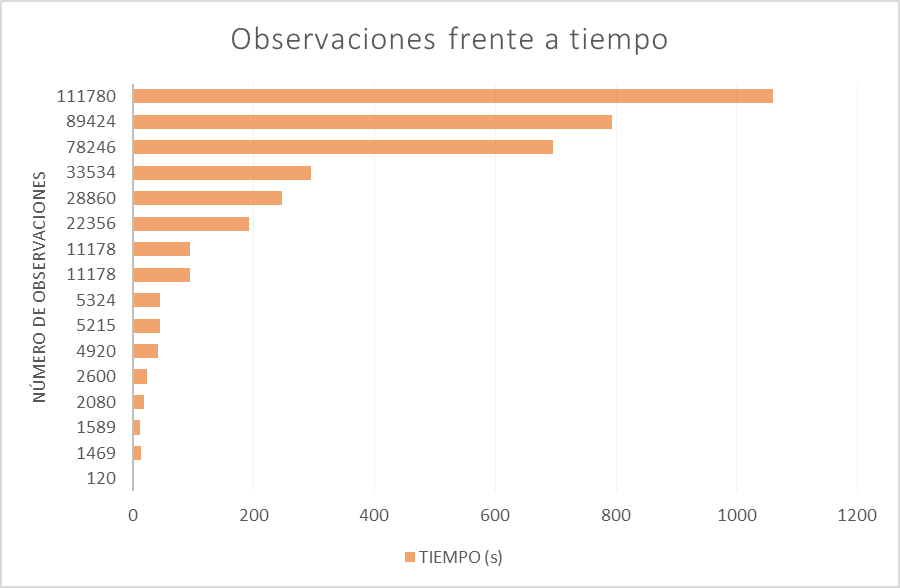
\includegraphics[width=0.8\textwidth]{mediciones/obs_vs_tiempo}
		\caption{Número de observaciones entrantes frente a tiempo de procesado}
		\label{fig:obs_vs_tiempo}
	\end{figure}
	
	\begin{figure}[h]
		\centering
		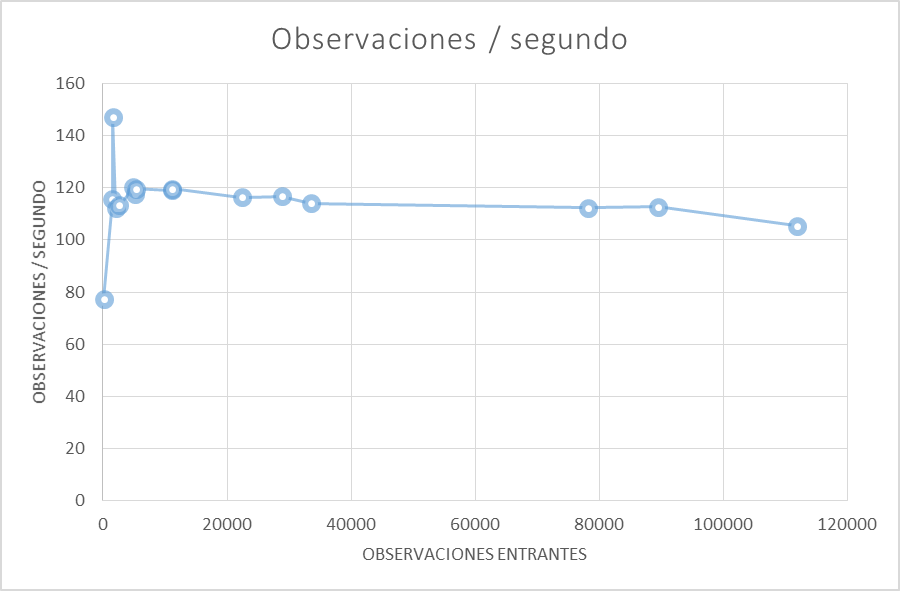
\includegraphics[width=0.8\textwidth]{mediciones/observaciones_segundo}
		\caption{Número de observaciones por segundo procesadas}
		\label{fig:obs_segundo}
	\end{figure}
	
	\begin{figure}[h]
		\centering
		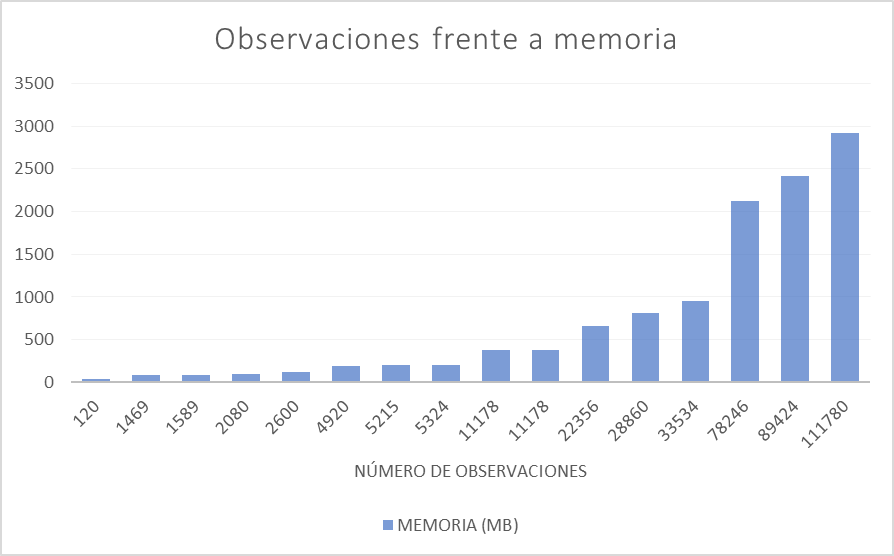
\includegraphics[width=0.8\textwidth]{mediciones/obs_vs_memoria}
		\caption{Número de observaciones frente a memoria durante el procesado}
		\label{fig:obs_vs_memoria}
	\end{figure}	
	 

\subsection{Análisis de los resultados}
	A continuación se expondrán las conclusiones extraídas de los resultados obtenidos durante las mediciones. Los resultados han sido expuestos en la tabla \ref{table:mediciones_receiver} y las figuras \ref{fig:obs_vs_tiempo}, \ref{fig:obs_segundo} y \ref{fig:obs_vs_memoria}.
	\begin{itemize}
		\item
			El número de observaciones del catálogo de datos entrante es el valor dominante en el consumo de tiempo y memoria durante el procesado de los datos.  Conforme aumenta el número de observaciones presentes en el catálogo de datos, el resto de factores (indicadores, usuario, etc) son despreciables.
		\item
			El número de observaciones entrantes es directamente proporcional tanto al tiempo como a la memoria utilizados durante el procesado de datos. 
		\item
			La velocidad de procesado de datos tiende a estabilizarse en torno a un valor concreto.  En el caso de la máquina en la que se realizaron las mediciones éste valor fue de 105 observaciones por segundo.
		\item
			El \textit{profiling} de memoria hace notablemente más lento el procesado de datos, por lo que la decisión de medir por separado el consumo de memoria y de tiempo ha sido positiva para evitar interferencias entre ambas mediciones.
		\item
			La complejidad del modelo de datos, así como el uso de un Mapeador Objeto-Relacional (ORM) para gestionar la persistencia obligan a crear multitud de objetos relacionados entre sí durante el parseo y la persistencia del catálogo de datos.  Ésto provoca el alto consumo de memoria mostrado en las mediciones, que en varias ocasiones llega a multiplicar por un factor de 70 el tamaño del catálogo de datos entrante.
	\end{itemize}



\section{Pruebas de aceptación}
\label{pruebas:aceptacion}

\chapter{Manuales del sistema}
\label{chapter08}
\section{Manual de instalación}
En esta sección se explicarán los pasos necesarios para instalar el sistema y todas las herramientas requeridas para su correcto funcionamiento.

El manual de instalación ha sido originalmente creado para el cliente y se encuentra disponible en el anexo ``\nameref{anexo_manual_instalacion}'' (escrito en inglés), perteneciente al capítulo \ref{anexos}.


\section{Manual de configuración}
Tras la instalación de todos los componentes del portal, será necesario realizar una configuración manual en la parte del gestor de contenidos.

Al igual que el manual de instalación, el manual de configuración ha sido originalmente creado para el cliente y se encuentra disponible en el anexo ``\nameref{anexo_manual_configuracion}'' (escrito en inglés) perteneciente al capítulo \ref{anexos}.

\section{Manual de usuario}
Dado que este proyecto consiste en la creación de un portal de datos, y no cuenta con una estructura compleja de cara al usuario como podría ser una doble interfaz de comunicación entre una parte web y una aplicación móvil, se ha optado por orientar el manual de usuario hacia una serie de preguntas y respuestas.
Estas preguntas y respuestas tratarán los temas que se han considerado más interesantes para los usuarios.

Al igual que el resto de manuales, ésta serie de preguntas y respuestas han sido originalmente creados para el cliente y se encuentran disponibles (escritas en inglés) en el anexo ``\nameref{anexo_manual_usuario}'' perteneciente al capítulo \ref{anexos}.

\chapter{Conclusiones y ampliaciones}
\label{chapter:conclusiones_ampliaciones}
En este capítulo se incluirán las conclusiones extraídas a lo largo del proyecto así como las posibles ampliaciones que se podrían llevar a cabo para aumentar el valor del sistema.

\section{Conclusiones}
\label{conclusiones}
Una vez finalizado el sistema es el momento de realizar una retrospectiva y extraer
conclusiones, tanto técnicas como personales.

En primer lugar, se han adquirido multitud de conocimientos en nuevos lenguajes y 
frameworks que nunca había utilizado antes de éste proyecto.  En concreto, el 
conocimiento de un nuevo lenguaje de programación no se limita únicamente al 
conocimiento de su sintaxis, si no que también incluye el conocimiento
de sus conceptos (por ejemplo: \textit{duck typing} en Python frente a tipado fuerte en Java)
y abstracciones (por ejemplo: \textit{list comprehensions} y \textit{generator expressions} en Python frente a bucles \textit{for}
y \textit{foreach} en PHP), y la forma de combinarlas para conseguir un resultado
adecuado.

También se ha comprendido la necesidad de evitar caer en la optimización prematura
durante el desarrollo.  La optimización prematura causa en multitud de ocasiones 
un aumento en la complejidad del código y, por tanto, en el riesgo de introducir nuevos
errores.  En relación con ésto, también se ha aprendido a utilizar un
\textit{profiler} para obtener distintas métricas objetivas sobre el funcionamiento del
programa y analizar así qué puntos requieren una optimización y que puntos 
funcionan adecuadamente.

El tamaño del sistema a desarrollar ha puesto de manifiesto los beneficios del
uso de una buena arquitectura que permita desacoplar los diferentes componentes.
Éste desacoplamiento entre los diferentes componentes ha facilitado su desarrollo
y hace también posible el remplazo de un componente por otro con mínimos cambios
en el resto del sistema.

Siendo éste el primer proyecto en el que participo como parte de un equipo de 
desarrollo y con un cliente real al que se destina el proyecto, ha sido muy
importante aprender a trabajar en equipo y a tomar decisiones sobre el sistema
de forma conjunta.  En relación con ésto, también ha sido importante tomar
responsabilidad sobre diversas partes del sistema y comprender que de su correcto
funcionamiento depende el trabajo del resto de miembros del equipo.

Dado que, como se ha dicho antes, éste es mi primer proyecto con un cliente real,
ha sido también necesario aprender a trabajar manteniendo hitos inamovibles 
(o \textit{deadlines}) y adoptando requisitos cambiantes.\\
En varias ocasiones durante el desarrollo se han tenido que tomar decisiones
para poder alcanzar un determinado hito, ésto me ha introducido al concepto de
\textit{deuda técnica}\footnote{El concepto de \textit{deuda técnica} fue creado por
Ward Cunningham para explicar el coste producido en el sistema por aquellas situaciones
en las que es necesario adelantar trabajo (aunque no sea de la forma más correcta) y
arreglar lo ya hecho (pagar la deuda técnica) posteriormente.  Para más información
sobre éste concepto se recomienda el artículo de Martin Fowler al respecto \cite{mfowler:technical_debt}},
sus beneficios e inconvenientes y la forma de utilizarlo en las situaciones que sea necesario.


En resumen, éste proyecto ha supuesto multitud de cambios para mí: desde cambios en
las herramientas y metodologías de desarrollo hasta cambios en la organización y
coordinación del trabajo.  Formar parte de un equipo de trabajo en el que todos
los compañeros superan mis conocimientos ha sido una gran lección tanto técnica como
personal, y aprender a aprovechar esa situación para crecer y mejorar en ambos sentidos
ha sido, sin ningún tipo de duda, un acierto.

\section{Ampliaciones}
\label{ampliaciones}
A continuación se enumerarán las posibles ampliaciones que se podrían realizar
para aumentar el valor y la funcionalidad del sistema.


\subsection{Incluir soporte a nuevas visualizaciones en el subsistema de datos}
	El framework de soporte a visualizaciones podría ser ampliado para facilitar
	la creación de nuevos tipos de visualizaciónes con las que enriquecer la
	sección del portal dedicada a los datos.

\subsection{Incluir soporte a nuevas redes sociales para iniciar sesión en el sistema}
	Actualmente el sistema soporta el inicio de sesión utilizando las redes sociales
	Twitter y Facebook.  Permitir el inicio de sesión en el portal utilizando nuevas
	redes sociales como Google+, LinkedIn o GitHub facilitaría el acceso a los
	usuarios.

\subsection{Facilitar el mecanismo de obtención de claves de acceso al API}
	Actualmente los usuarios que quieran obtener una clave de acceso al API
	deben enviar un correo electrónico a la administración del portal, para que
	sea el administrador quien modifique el rol del usuario y le permita obtener
	su clave de aceso al API.
	
	Una ampliación interesante para los usuarios 
	consistiría en permitirles solicitar una nueva clave de acceso al API
	de forma automática desde la vista de su perfil de usuario.

\subsection{Gestión automática de los debates}
	Actualmente es la administración del portal quien se encarga de abrir y cerrar
	los debates cuando se alcance su periodo de participación.
	
	Una ampliación
	destinada a gestionar automáticamente la apertura y el cierre de los debates
	facilitaría la tarea de los administradores, sobre todo cuando el número de
	debates existentes es muy alto.

\subsection{Migración del contenido desde el viejo LandPortal}
	El viejo LandPortal cuenta con una gran cantidad de información creada por sus
	usuarios a lo largo del tiempo.  Una posible ampliación consistiría en migrar
	dicha información desde el viejo al nuevo portal.
	
	La tésis de Alan Chavoshe, titulada ``Linked Data for the Land Portal''
	\cite{lod_landportal}, contiene una explicación detallada de la estructura con la
	que se almacenan los datos en el viejo Land Portal.	Atendiendo a lo expuesto 
	en dicha tésis, el modelo de datos del viejo Land Portal difiere bastante
	del modelo utilizado en éste proyecto.  
	
	El primer paso para realizar ésta migración requeriría crear un nuevo módulo
	que extienda del módulo \textit{migrate}\footnote{El módulo \textit{migrate}
	es un módulo de Drupal destinado a facilitar la migración de contenidos 
	entre distintos portales.  El módulo \textit{migrate} esta disponible en
	\url{https://www.drupal.org/project/migrate}}.
	
	El mayor problema provendría de los tipos de contenido que no existen en 
	el nuevo portal como:  \textit{OrganisationType}, \textit{GPL Drivers} o
	\textit{Expertise}.  Para migrar éste tipo de contenidos sería necesario
	modificar la estructura de datos del nuevo Land Portal y modificar también
	las vistas correspondientes para presentarlos a los usuarios.
	
	Una primera estimación sobre el tiempo necesario para realizar ésta ampliación
	sería entre 100 o 150 horas, en las que modificar las estructuras del modelo
	de datos y las vistas necesarias.
	
\subsection{Futuros proyectos con el IFAD}
	Además de las posibles ampliaciones detalladas anteriormente, también existen una
	serie de futuros proyectos que se realizarán con el mismo cliente.
	\begin{itemize}
		\item Un \textit{hackatón}\footnote{Un \textit{hackatón} o \textit{hackathon} es un encuentro de programadores destinado a realizar un desarrollo colaborativo de software} para la creación de nuevos componentes del portal.  Concretamente
		el \textit{hackatón} consistiría en crear nuevos importadores para incluir catálogos de
		datos en el portal y nuevas visualizaciones con las que presentar los datos
		ya existentes.\\
		Originalmente el hackatón ha sido planteado para tener lugar durante el verano
		de 2014 en Alemania.
		
		\item Creación de la biblioteca o LandLibrary.  El LandLibrary es la tercera
		sección del portal y tiene como objetivo ser un repositorio de documentos,
		publicaciones, estudios, mapas, etc.  El LandLibrary tendrá también	capacidad
		de búsqueda y contará con un enriquecimiento semántico de los metadatos de
		las publicaciones que albergue.
		
		La información almacenada en el LandLibrary se hará pública en forma de
		datos enlazados abiertos para ser utilizados por servicios de terceros y 
		para ser incluidos en diferentes partes del portal, concretamente en el
		LandBook.
		
		Por su gran tamaño, ésta ampliación tendrá lugar como un proyecto con
		entidad propia.  Éste proyecto está planificado para comenzar en otoño
		del 2014.
		
	\end{itemize}



\chapter{Anexos}
\label{anexos}
\section{Installation manual}
\label{anexo_manual_instalacion}
For a successful system installation the following elements are required:


\begin{itemize}
	\item \textbf{Installation scripts}.  To facilitate the installation task, and since this system has multiple internal and third-party components,  the developers have created a series of scripts that automate the system installation.
	\item \textit{GNU/Linux distribution}.  The installation scripts have been only tested under Ubuntu 14.04 LTS, so it is highly recommended to use this distribution for the system deployment.
\end{itemize}

The first step consists of logging into the system with a non-root account.  The non-root account is important because the file paths in the scripts are relative to the user's home directory, the root home directory is \textit{/root} while the home directory for regular users is \textit{/home/USERNAME}.

Once you have logged into the system with a non-root account, the following step consists of copying the content of the scripts folder into the user's home directory.  Such as in the image \ref{fig:manual_instalacion_home}, the files \textit{install.sh} and \textit{settings.ph} and the folders \textit{scripts} and \textins{solr} must be located into the root of the user's home directory.

\begin{figure}[h]
	\centering
	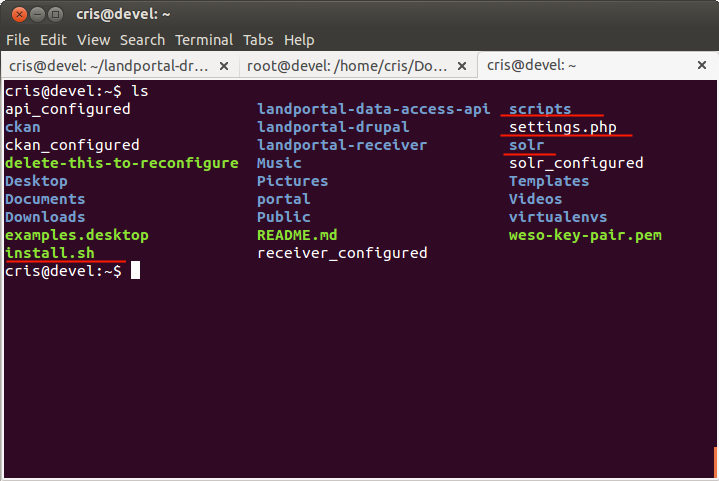
\includegraphics[width=\textwidth]{manual_instalacion/home_folder}
	\caption{User's home folder with the script files (underlined in red)}
	\label{fig:manual_instalacion_home}
\end{figure}

After copying the installation scripts into the home directory, the system installation can be easily triggered with the command \textit{sudo ./install.sh}, which means to run the script \textit{install.sh}, which is located into the current directory, with superuser privileges.  The superuser privileges are required to install some packages and configurations.  The image \ref{fig:manual_instalacion_lanzamiento} shows the command before starting the installation.

When you hit the \textit{enter} key, the installation will begin.  The installation process is completely automated and requires no user interaction, but since it is such a big system, the installation can last a long time.

After the installation ends, the system is completely functional, but it still needs some configuration.  Please, take a look into the ``\nameref{anexo_manual_configuracion}''.

\begin{figure}[h]
	\centering
	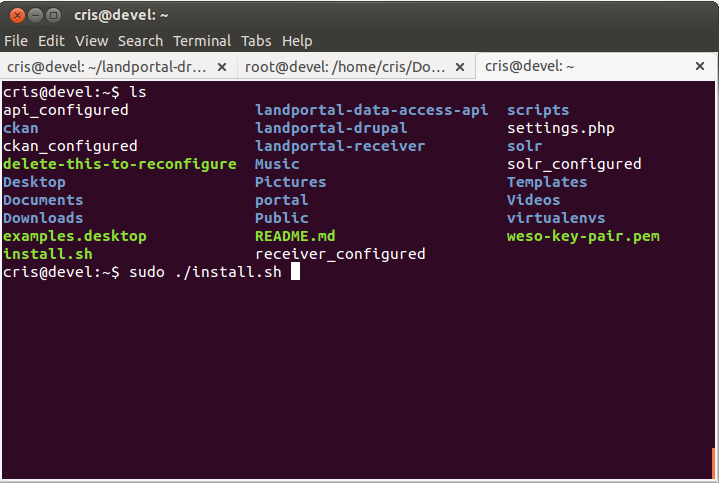
\includegraphics[width=\textwidth]{manual_instalacion/launch_installation}
	\caption{Launch system installation command}
	\label{fig:manual_instalacion_lanzamiento}
\end{figure}

\section{Configuration manual}
\label{anexo_manual_configuracion}

\printbibliography

\end{document}
